%\documentclass[tikz]{report}
\documentclass{book}



\usepackage{minted}
\usepackage{listings}




\usepackage[dvipsnames]{xcolor}
\usepackage{lmodern}
\usepackage[all]{xy}
\usepackage[brazil]{babel}
\usepackage[utf8]{inputenc}

\usepackage{amssymb}
\usepackage{amsmath}
\usepackage{amsthm}
\usepackage{amscd}
\usepackage{amsfonts}
\usepackage{mathrsfs}
\usepackage{mathtools}
\usepackage{mathabx}

\usepackage{pst-node}
\usepackage{tikz-cd}
\usepackage{tikz}
\usepackage{forest}
\usepackage{caption}
\usepackage{subcaption}
\usepackage{float}
\usetikzlibrary{shadows,shapes.geometric}
\usetikzlibrary{calc}
\usepackage{enumerate}
\usepackage{times}
\usepackage[pdftex]{hyperref}
\usepackage[most]{tcolorbox}
\usepackage{titletoc}
\usepackage{moresize}

\usepackage{anyfontsize}


\usepackage{erewhon}
\usepackage{titlesec}
\usepackage{epigraph}% Pacotes usados
\theoremstyle{plain}
\newtcbtheorem[number within=chapter]{prob}{\strut Exercício}{
    enhanced,
    colframe=BlueViolet!75,
    colback=white,
    colbacktitle=BlueViolet!75,
    coltitle=white,
    boxed title style={},
    attach boxed title to top left={xshift=5mm,yshift*=-\tcboxedtitleheight/2},
    before skip=25pt plus 2pt,
    after skip=15pt plus 2pt
}{th}

\newtcbtheorem[number within=chapter]{teo}{\strut Teorema}{
    enhanced,
    colframe=BlueViolet!75,
    colback=white,
    colbacktitle=BlueViolet!75,
    coltitle=white,
    boxed title style={},
    attach boxed title to top left={xshift=5mm,yshift*=-\tcboxedtitleheight/2},
    before skip=25pt plus 2pt,
    after skip=15pt plus 2pt
}{th}

\newtcbtheorem[number within=chapter]{df}{\strut Definição}{
    enhanced,
    colframe=BlueViolet!75,
    colback=white,
    colbacktitle=BlueViolet!75,
    coltitle=white,
    boxed title style={},
    attach boxed title to top left={xshift=5mm,yshift*=-\tcboxedtitleheight/2},
    before skip=25pt plus 2pt,
    after skip=15pt plus 2pt
}{th}

\newtcbtheorem[number within=chapter]{prop}{\strut Proposição}{
    enhanced,
    colframe=BlueViolet!75,
    colback=white,
    colbacktitle=BlueViolet!75,
    coltitle=white,
    boxed title style={},
    attach boxed title to top left={xshift=5mm,yshift*=-\tcboxedtitleheight/2},
    before skip=25pt plus 2pt,
    after skip=15pt plus 2pt
}{th}

\newtcbtheorem[number within=chapter]{coro}{\strut Corolário}{
    enhanced,
    colframe=BlueViolet!75,
    colback=white,
    colbacktitle=BlueViolet!75,
    coltitle=white,
    boxed title style={},
    attach boxed title to top left={xshift=5mm,yshift*=-\tcboxedtitleheight/2},
    before skip=25pt plus 2pt,
    after skip=15pt plus 2pt
}{th}

\newtcbtheorem[number within=chapter]{lema}{\strut Lema}{
    enhanced,
    colframe=BlueViolet!75,
    colback=white,
    colbacktitle=BlueViolet!75,
    coltitle=white,
    boxed title style={},
    attach boxed title to top left={xshift=5mm,yshift*=-\tcboxedtitleheight/2},
    before skip=25pt plus 2pt,
    after skip=15pt plus 2pt
}{th}

\theoremstyle{definition}
\newtheorem{ex}{Exemplo}% Definição das estruturas de teorema
\titleformat{\chapter}[block]%
        {\normalfont\scshape\HUGE}%
        {\hspace*{-70pt}\color{BlueViolet!75}\fontencoding{U}\fontfamily{eur}\fontseries{b}\fontsize{60}{80}\selectfont\thechapter\hspace{15pt}}{10pt}
        {}[\chapterdecoration]

\newcommand\chapterdecoration{%
\begin{tikzpicture}[remember picture,overlay,shorten >= -10pt]

\coordinate (aux1) at ([yshift=-15pt]current page.north east);
\coordinate (aux2) at ([yshift=-410pt]current page.north east);
\coordinate (aux3) at ([xshift=-4.5cm]current page.north east);
\coordinate (aux4) at ([yshift=-150pt]current page.north east);

\begin{scope}[BlueViolet!50,line width=12pt,rounded corners=12pt]
\draw
  (aux1) -- coordinate (a)
  ++(225:5) --
  ++(-45:5.1) coordinate (b);
\draw[shorten <= -10pt]
  (aux3) --
  (a) --
  (aux1);
\draw[opacity=0.6,BlueViolet,shorten <= -10pt]
  (b) --
  ++(225:2.2) --
  ++(-45:2.2);
\end{scope}
\draw[BlueViolet,line width=8pt,rounded corners=8pt,shorten <= -10pt]
  (aux4) --
  ++(225:0.8) --
  ++(-45:0.8);
\begin{scope}[BlueViolet!70,line width=6pt,rounded corners=8pt]
\draw[shorten <= -10pt]
  (aux2) --
  ++(225:3) coordinate[pos=0.45] (c) --
  ++(-45:3.1);
\draw
  (aux2) --
  (c) --
  ++(135:2.5) --
  ++(45:2.5) --
  ++(-45:2.5) coordinate[pos=0.3] (d);   
\draw 
  (d) -- +(45:1);
\end{scope}
\end{tikzpicture}%
}


\everymath{\displaystyle}

\setlength{\parindent}{0em}
\renewcommand{\baselinestretch}{1.5}

% não permite separação silábica
\sloppy
\hyphenpenalty=100000
% não permite linhas orfãs e viúvas no tex
\clubpenalty=10000
\widowpenalty=10000
\displaywidowpenalty=10000% Configurações de formatação
\newcommand{\tituloum}[5]{\begin{titlepage} 
    \pagecolor{BlueViolet}
    \color{white}
	\centering 
	
	\scshape 
	
	\vspace*{\baselineskip}

	
	\rule{\textwidth}{1.6pt}\vspace*{-\baselineskip}\vspace*{2pt} 
	\rule{\textwidth}{0.4pt} 
	
	\vspace{0.75\baselineskip} 
	
	{\LARGE #1} 
	
	\vspace{0.75\baselineskip}
	
	\rule{\textwidth}{0.4pt}\vspace*{-\baselineskip}\vspace{3.2pt}
	\rule{\textwidth}{1.6pt}
	
	\vspace{2\baselineskip}
	
	#2
	
	\vspace*{3\baselineskip}
	
	Autor
	
	\vspace{0.5\baselineskip}
	
	{\scshape\Large #3}
	
	\vspace{0.5\baselineskip}
	
	\textit{#4}
	
	\vfill
	
	\vspace{0.3\baselineskip}
	
	#5

\end{titlepage}
\nopagecolor}% Comandos definidos
\titlecontents{chapter}[0pc]
{\addvspace{30pt}}%
{\begin{tikzpicture}[remember picture, overlay]%
\draw[fill=BlueViolet!80,draw=BlueViolet!80] (-4,-.2) rectangle (-0.5,.5);%
\pgftext[left,x=-3.6cm,y=0.2cm]{\color{white}\Large\sc\bfseries capítulo\                                             
\thecontentslabel};%
\end{tikzpicture}\color{BlueViolet!90}\large\sc\bfseries}
{\color{BlueViolet!90}\large\sc\bfseries}
{\color{BlueViolet!90}\;\titlerule\;\large\sc\bfseries Página \thecontentspage
\begin{tikzpicture}[remember picture, overlay]
\draw[fill=BlueViolet!70,draw=BlueViolet!70] (2pt,0) rectangle (6,0.1pt);
\end{tikzpicture}}%

\titlecontents{section}[2.4pc]
{\addvspace{1pt}}
{\contentslabel[\thecontentslabel]{2.4pc}}
{}
{\dotfill\small \thecontentspage}
[]
\titlecontents{subsection}[5pc]
{\addvspace{1pt}}
{\contentslabel[\thecontentslabel]{2.4pc}}
{}
{\dotfill\small \thecontentspage}
[]
\makeatletter

\renewcommand{\tableofcontents}{%
\chapter*{%
\vspace*{-20\p@}%
\begin{tikzpicture}[remember picture, overlay]%
\pgftext[right,x=14.84cm,y=0.2cm]{\color{BlueViolet!80}\Huge\sc\bfseries    
\contentsname};%
\draw[fill=BlueViolet!80,draw=BlueViolet!80] (13,-.75) rectangle (20,1);%
\clip (13,-.75) rectangle (20,1);
\pgftext[right,x=14.84cm,y=0.2cm]{\color{white}\Huge\sc\bfseries 
\contentsname};%
\end{tikzpicture}}%
\@starttoc{toc}}
\makeatother

\everymath{\displaystyle}

\begin{document}



%MODELO DA CAPA 1:
\tituloum
{Sistemas Computacionais}
{Notas de aula}
{G. A., Davi; A. P., Lourenço.}
{Instituição}
{2022}

%MODELO DE CAPA 2:
%\begin{titlepage}
\pagestyle{empty}

% Background color
\begin{tikzpicture}[remember picture,overlay]
\fill[BlueViolet] (current page.south west) rectangle (current page.north east);


% Background Hexagon
\begin{scope}
\foreach \i in {2.5,...,22}
{\node[rounded corners,BlueViolet!90,draw,regular polygon,regular polygon sides=6, minimum size=\i cm,ultra thick] at ($(current page.west)+(2.5,-5)$) {} ;}
\end{scope}

\foreach \i in {0.5,...,22}
{\node[rounded corners,BlueViolet!90,draw,regular polygon,regular polygon sides=6, minimum size=\i cm,ultra thick] at ($(current page.north west)+(2.5,0)$) {} ;}

\foreach \i in {0.5,...,22}
{\node[rounded corners,BlueViolet!98,draw,regular polygon,regular polygon sides=6, minimum size=\i cm,ultra thick] at ($(current page.north east)+(0,-9.5)$) {} ;}

\foreach \i in {21,...,6}
{\node[BlueViolet!95,rounded corners,draw,regular polygon,regular polygon sides=6, minimum size=\i cm,ultra thick] at ($(current page.south east)+(-0.2,-0.45)$) {} ;}

% Title of the Report
\node[left,BlueViolet!5,minimum width=0.625*\paperwidth,minimum height=3cm, rounded corners] at ($(current page.north east)+(0,-9.5)$){{\fontsize{25}{30} \selectfont \bfseries Título}};

% Subtitle 
\node[left,BlueViolet!10,minimum width=0.625*\paperwidth,minimum height=2cm, rounded corners] at ($(current page.north east)+(0,-11)$){{\textit{Instituição}}};

% Author Name
\node[left,BlueViolet!5,minimum width=0.625*\paperwidth,minimum height=2cm, rounded corners] at ($(current page.north east)+(0,-13)$){{\Large \textsc{Autor}}};

% Year
\node[rounded corners,fill=BlueViolet!95,text =BlueViolet!5,regular polygon,regular polygon sides=6, minimum size=2.5 cm,inner sep=0,ultra thick] at ($(current page.west)+(2.5,-5)$) {\LARGE \bfseries Ano};

\end{tikzpicture}
\end{titlepage}

\thispagestyle{empty}
%Você pode botar qualquer descrição aqui: BLA BLA BLA BLA BLA BLA BLA BLA BLA BLA BLA BLA BLA BLA BLA BLA BLA BLA BLA BLA BLA BLA BLA BLA BLA BLA BLA BLA BLA BLA BLA BLA BLA BLA BLA BLA BLA BLA BLA BLA BLA BLA BLA BLA BLA BLA BLA BLA BLA BLA BLA BLA BLA BLA BLA BLA BLA BLA BLA BLA BLA BLA BLA BLA BLA BLA BLA BLA BLA BLA BLA BLA BLA BLA BLA BLA BLA BLA BLA BLA BLA BLA BLA BLA BLA BLA BLA BLA BLA BLA BLA BLA BLA BLA BLA BLA BLA BLA BLA BLA BLA BLA BLA BLA BLA BLA BLA BLA BLA BLA BLA BLA BLA BLA BLA BLA BLA BLA BLA BLA BLA BLA BLA BLA BLA BLA BLA BLA BLA BLA BLA BLA BLA BLA BLA BLA BLA BLA BLA BLA BLA BLA BLA BLA BLA BLA BLA BLA BLA BLA BLA BLA BLA BLA BLA BLA BLA BLA BLA BLA BLA BLA%pode omitir a descrição apagando essa linha
\pagenumbering{roman}
\tableofcontents

\newpage

\pagenumbering{arabic}
%\chapter{Capítulo}

\begin{df}[]{}{}
Esta é uma definição.
\end{df}

\begin{lema}[]{}{}
Este é um lema.
\end{lema}

\begin{prop}[]{}{}
Esta é uma proposição.
\end{prop}

\begin{teo}[]{Teorema muito importante}{}
Este é um teorema.
\end{teo}

\begin{proof}
Exercício para o leitor.
\end{proof}

\begin{coro}[]{}{}
Este é um corolário.
\end{coro}

\begin{ex}
um simples exemplo.
\end{ex}

% XeLaTeX can use any Mac OS X font. See the setromanfont command below.
% Input to XeLaTeX is full Unicode, so Unicode characters can be typed directly into the source.

% The next lines tell TeXShop to typeset with xelatex, and to open and save the source with Unicode encoding.

%!TEX TS-program = xelatex
%!TEX encoding = UTF-8 Unicode





% Will Robertson's fontspec.sty can be used to simplify font choices.
% To experiment, open /Applications/Font Book to examine the fonts provided on Mac OS X,
% and change "Hoefler Text" to any of these choices.



% - Sistemas Operacionais




\hypertarget{sistemas-operacionais}{%
\chapter{Sistemas Operacionais}\label{sistemas-operacionais}}



\hypertarget{Introdução}{%
\section{Introdução}\label{Introdução}}

O Sistema Operacional (SO) é um software que gerencia os recursos de
hardware e os tornam simples de serem usados por aplicações. Esse
gerenciamento é feito pelo núcleo, ou \texttt{Kernel}, do SO, o qual tem
permissões especiais de uso. As aplicações criadas pelos usuários se
encontram no \texttt{User Space}, um local com abstrações para o fácil uso desses
recursos. A mudança do espaço pode ser requisitada pela aplicação, com
um processo chamado de \texttt{trap}, o qual faz referência à uma
interceptação, como cair no alçapão de uma casa, tendo assim acesso ao
subterrâneo, no caso o núcleo do SO. Esse processo passa pelas chamadas
de sistema (System Calls), as quais são uma interface de comunicação
entre o espaço de usuário e o \texttt{kernel}. As aplicações no espaço de usuário
contam com as abstrações GNU libc, uma biblioteca que segue o padrão
POSIX, e outros, de normas de compatibilidade entre os sistemas
operacionais, tornando, assim, os programas portáteis. Outras abstrações
importantes são a de processos, que são programas em execução, e a de
\texttt{File System} (FS), responsável por gerenciar os arquivos, usando, por
exemplo, diretórios para agrupá-los. A inicialização do sistema
computacional começa pelo carregamento do BIOS (\emph{Basic Input Output
System}), o qual é armazenado em uma memória flash (uma EEPROM, ou
\emph{Electrically Erasable and Programmable Read Only Memory}) na placa
mãe, e é encarregado por tarefas básicas de gerenciamento do hardware,
como o POST (\emph{Power On Self Test}), processo incumbido por verificar
o estado operacional do sistema. O BIOS também é responsável por
carregar o SO, da memória secundária para a memória primária, processo
que finaliza com o sistema operacional assumindo o controle do hardware.
A memória primária, ou RAM (\emph{Random Access Memory}), é uma memória
volátil (não mantém os dados após o cessamento da energia) de acesso
direto ao processador. Os programas necessitam estar nessa memória para
serem executados. Já a memória secundária, também chamada de Drive (ou
disco), passa por um sistema I/O (\emph{Input Output}), o qual é
encarregado por gerenciar a entrada e saída de dados com outros
dispositivos. A Figura \ref{fig:sistema computacional} mostra como as subdivisões de um sistema
computacional, destacando as do sistema operacional.

\begin{figure}[h]
\centering
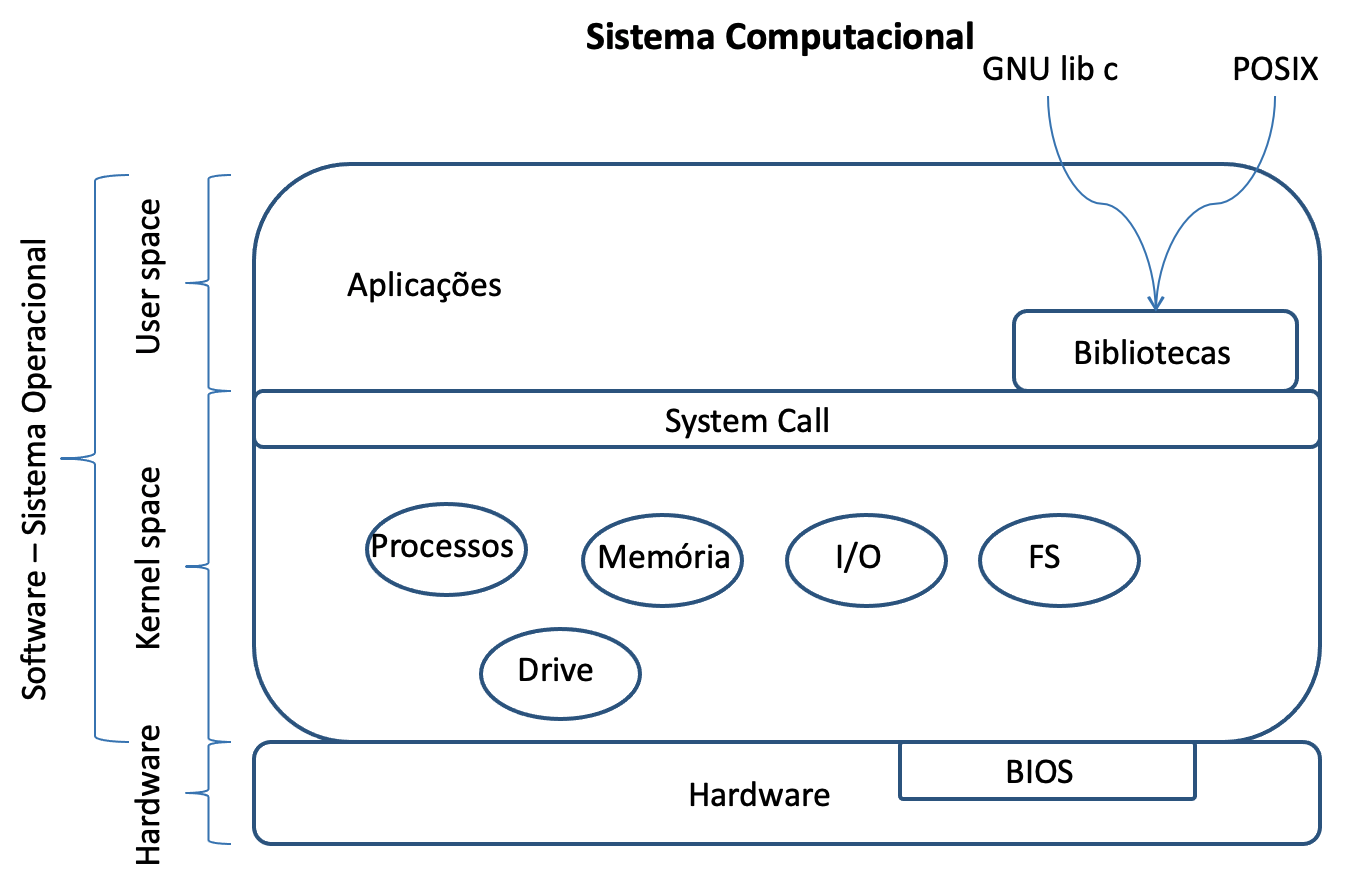
\includegraphics[keepaspectratio, width=12cm, height=9cm]{imagens/02/02 - funcionamento do computador.png}
\caption{Sistema Computacional}
\label{fig:sistema computacional}
\end{figure}



\hypertarget{Prática}{%
\section{Prática}\label{Prática}}

Com o intuito de mostrar como funciona as chamadas do sistema e como
funciona a compilação, vamos criar um programa \texttt{Hello\ world} na
linguagem C. Para tal, precisamos entender alguns comandos do Linux.

\hypertarget{comandos-linux}{%
\subsubsection{Comandos Linux}\label{comandos-linux}}

\begin{enumerate}
\def\labelenumi{\arabic{enumi}.}
\tightlist
\item
  \texttt{mkdir}: cria um novo diretório
\item
  \texttt{grep}: procura um texto em um arquivo
\item
  \texttt{rm}: remover um arquivo
\item
  \texttt{mv}: move o arquivo
\item
  \texttt{ls}: lista os elementos de um diretório
\item
  \texttt{ls\ -a}: lista arquivos
\item
  \texttt{ls\ -l}: lista permissões
\item
  \texttt{ls\ -F}: edita os nomes, como \texttt{*} no final do nome dos
  arquivos executáveis
\item
  \texttt{ls\ -F}: edita os nomes, como \texttt{*} no final do nome dos
  arquivos executáveis
\item
  \texttt{ll}: um alias para \texttt{ls\ -alF}
\item
  \texttt{file}: inspecionar um arquivo
\item
  \texttt{cd}: mudar o diretório
\item
  \texttt{ld}: vinculador, responsável por gerar um arquivo executável a
  partir de um objeto
\item
  \texttt{objdump}: Mostra informações sobre um arquivo objeto
\item
  \texttt{objdump\ -d}: desmota (disassembly) um arquivo objeto.
  
        \begin{lstlisting}[language=bash]
            $ objdump -d file.o
        \end{lstlisting}


\item
  \texttt{Vim}: Vi Improved -- Editor de texto. \texttt{\$vim\ file}
  
        \begin{lstlisting}[language=bash]
            $ vim file
        \end{lstlisting}
\item
  \texttt{Vi}: Editor de texto.
\item
  \texttt{-o}: output -- resultado de um comando
\item
  \texttt{as}: compilador assembly
\item
  \texttt{gcc}: compilador GNU para a linguagem C, gera arquivo
  executável a partir de um arquivo \texttt{.c}.

        \begin{lstlisting}[language=bash]
            $ gcc file.c -o file
        \end{lstlisting}  
  
\item
  \texttt{gcc\ -E}: gera arquivo pré-processado (\texttt{.pre}).
 
  
        \begin{lstlisting}[language=bash]
            $ gcc -E file.c -o file.pre
        \end{lstlisting}  
\item
  \texttt{gcc\ -S}: gera arquivo assembly (\texttt{.s})


        \begin{lstlisting}[language=bash]
            $ gcc -S file.c -o file.s
        \end{lstlisting}  
  
\item
  \texttt{gcc\ -c}: converte em linguagem de máquina sem vincular,
  gerando um arquivo objeto não executável (\texttt{.o})

        \begin{lstlisting}[language=bash]
            $ gcc -c file.c -o file.o
        \end{lstlisting}    
  
\item
  \texttt{man\ \#}: mostra o manual de uma função de alguma sessão


        \begin{lstlisting}[language=bash]
            $ man 3 printf
        \end{lstlisting}      
  
\item
  \texttt{man\ man}: mostra o manual do man
\item
  \texttt{echo}: mostra o texto resultado na saída padrão.
\item
  \texttt{./} : executa um arquivo executável
\end{enumerate}

\hypertarget{etapas-de-compilauxe7uxe3o}{%
\subsection{Etapas de compilação}\label{etapas-de-compilauxe7uxe3o}}

O processo de compilação de um código está relacionado com transformar
um arquivo texto de uma linguagem específica, para um arquivo binário
executável. O compilador da linguagem C usado no Linux, \texttt{gcc},
realiza esse processo em 4 etapas. A primeira dessas etapas é o
pré-processamento, responsável por lidar com as diretivas de
pré-processamento, como o \texttt{\#include} e \texttt{\#define}, que
anexa um arquivo e substitui os macros, respectivamente. Tem como
resultado um arquivo de extensão pre (\texttt{.pre}). A segunda etapa é
a conversão do arquivo pré-processado para o assembly. Ela utiliza o
\emph{toolchain}, pacote de ferramentas contendo instruções específicas
do processador de destino, como ARM. A saída é um arquivo de extensão s
(\texttt{.s}). A terceira etapa é a geração de um código objeto em
binário, o qual é um arquivo de extensão o (\texttt{.o}). Por fim, há a
vinculação (\emph{linking}) do código objeto gerado na etapa anterior
com outros códigos objetos a fim de substituir as referências à símbolos
definidos fora do código objeto original. Tem como saída um arquivo
binário executável sem extensão. A Figura \ref{fig:Etapas de compilação do gcc} mostra as etapas de
compilação do gcc.

\begin{figure}[h!]
\centering
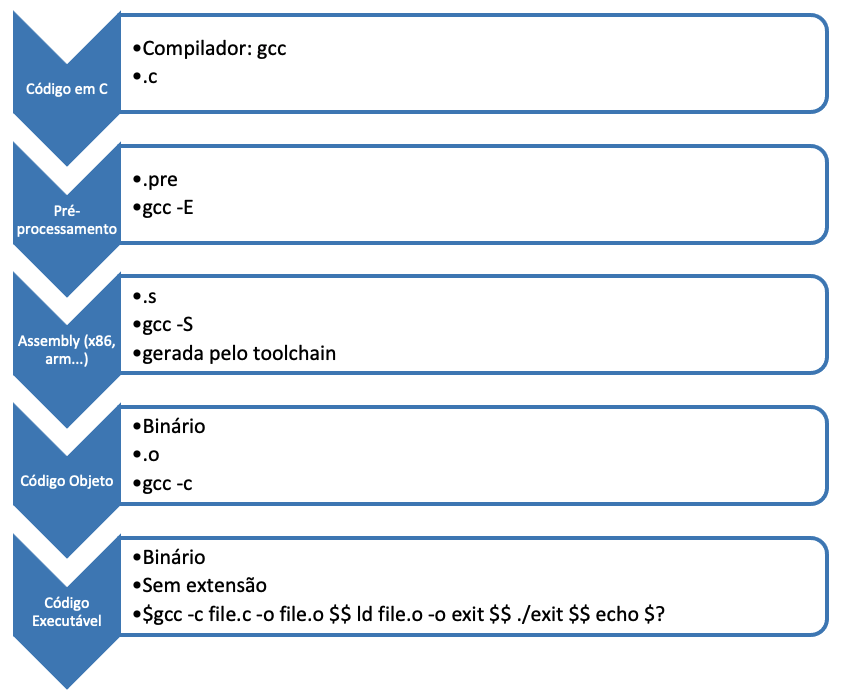
\includegraphics[width=12cm, height=9cm]{imagens/02/02 - compilação.png}
\caption{Etapas de compilação do gcc}
\label{fig:Etapas de compilação do gcc}
\end{figure}




\hypertarget{compilando-um-arquivo-.c}{%
\section{\texorpdfstring{Compilando um arquivo
\texttt{.c}}{Compilando um arquivo .c}}\label{compilando-um-arquivo-.c}}

A seguir será mostrado um passo a passo, da criação de um arquivo
\texttt{.c} até sua compilação.

Dentro do editor de texto Linux, escreva o código \texttt{Hello\ World}
disponível a seguir.

\begin{minted}[mathescape, linenos]{c}

    #include <stdio.h>
    int main() { 
        printf("Hello World!\n); 
        return 0; 
    }

\end{minted}



Salve com o nome \texttt{hw.c} Abra o terminal, vá até o diretório no
qual foi salvo o arquivo \texttt{hw.c}, e digite:


\begin{lstlisting}[language=bash]
  $ gcc hw.c -o hw
  $ ./hw
\end{lstlisting}





Será assim gerado um arquivo \texttt{hw} executável, com sua execução em
seguida.

Com o \texttt{gcc}, pode-se também gerar os arquivos das etapas
explicadas anteriormente, com 1, 2 e 3 gerando os arquivos
pré-processados, arquivo assembly e código objeto, respectivamente.





\begin{minted}[mathescape, linenos]{bash}

    $ gcc -E hw.c -o hw.pre
    $ gcc -S hw.c -o hw.s
    $ gcc -c hw.c -o hw.o
\end{minted}



É possível também ler o código objeto no formato de assembly com a
função de desassembly:

\begin{minted}[mathescape, linenos]{language=bash}

    $ objdump -d hw.o
    
    hw.o:     file format elf64-x86-64
    
    
    Disassembly of section .text:
    
    0000000000000000 <main>:
       0:   f3 0f 1e fa             endbr64
       4:   55                      push        %rbp
       5:   48 89 e5                mov         %rsp,%rbp
       8:   48 8d 3d 00 00 00 00    lea         0x0(%rip),%rdi  # f <main+0xf>
       f:   b8 00 00 00 00          mov         $0x0,%eax
      14:   e8 00 00 00 00          callq       19 <main+0x19>
      19:   b8 00 00 00 00          mov         $0x0,%eax
      1e:   5d                      pop         %rbp
      1f:   c3                      retq
\end{minted}


\hypertarget{executando-uma-chamada-do-sistema}{%
\section{Executando uma chamada do
sistema}\label{executando-uma-chamada-do-sistema}}

Para executar uma chamada do sistema, vamos, primeiro, criar um arquivo
assembly (\texttt{.s}) chamado de \texttt{01-exit64.s} com o conteúdo
abaixo:

\begin{minted}[mathescape, linenos]{assembly}
    
    .section .data
    .section .text
    .globl _start
    
    _start:
    
    
    # C code
    # exit(0);
        # mnemonic  # parameters    # comments
        movq        $60, %rax   # system call exit(2)
        movq        $10, %rdi   # the shell will receive this value
    
        syscall
\end{minted}



Após isso, devemos gerar um código objeto, usando um compilador assembly:

\begin{lstlisting}[language=bash]
    $ as 01-exit64.s -o exit.o
\end{lstlisting}



Depois gerar um arquivo executável, pelo processo de vinculação:


\begin{lstlisting}[language=bash]
    $ ld exit.o -o exit
\end{lstlisting}


Para executar e visualizar, basta digitar:


\begin{lstlisting}[language=bash]
    $ ./exit
    $ echo $?
\end{lstlisting}



\hypertarget{entendendo-system-call}{%
\subsection{Entendendo System Call}\label{entendendo-system-call}}

Para entender melhor o resultado gerado anteriormente, podemos acessar o
manual do system call com:


\begin{lstlisting}[language=bash]
    $ man syscall
\end{lstlisting}



A primeira tabela do manual será parecida com a tabela a seguir:




\begin{table}[h!]
\centering
\begin{tabular}{||c c c c c c||} 
 \hline
    Arch / ABI & Instruction & System Call # & val & val 2 & Error \\ [0.5ex] 
 \hline\hline
arm64 & svc \#0 & x8 & 0 & x1 & - \\
 \hline
 i386 & int \$0x80 & eax & ax & edx & - \\
 \hline
 mips & syscall & v0 & 0 & v1 & a3 \\
 \hline
 riscv & ecall & a7 & 0 & a1 & - \\
 \hline
 x86-64 & syscall & rax & ax & rdx & - \\
 \hline
 x32 & syscall & a2 & 2 & - & - \\
 \hline

\end{tabular}


 \caption{System Call por Arquitetura}
\label{tab:System Call por Arquitetura}
\end{table}


A Tabela \ref{tab:System Call por Arquitetura} mostra que para que a função syscall de um processador com
arquitetura x86-64 seja chamada, devemos primeiro ajustar o registrador
rax com o valor equivalente à função desejada. No exemplo dado, o valor
60 se refere a função ``exit'', que encerra a execução de um programa.
As diferentes funções e seus respectivos valores podem ser acessados em:

\url{https://elixir.bootlin.com/linux/latest/source/arch/x86/entry/syscalls/syscall\_64.tbl}

A Tabela \ref{tab:Argumentos das chamadas do sistema} mostra que o primeiro argumento a ser usado na arquitetura
x86-64 deve ser passado para o registrador rdi. A tabela completa pode
ser encontrada no manual do syscall. O valor passado para esse
registrador será retornado pelo syscall.



\begin{table}[h!]
\centering
\begin{tabular}{||c c c c c c c c c||} 
 \hline
    Arch / ABI & rg1 & rg2 & rg3 & rg4 & rg5 & rg6 & rg7 & notes \\ [0.5ex] 
 \hline\hline
x86-64 & rdi & rsi & rdx & r10 & r8 & r9 & - & \\

 \hline

\end{tabular}

 \caption{Argumentos das chamadas do sistema}
\label{tab:Argumentos das chamadas do sistema}
\end{table}

\somestuffstyle{movq}
A função \texttt{movq}, utilizada no programa assembly, move o valor
especificado para um dado registrador. No exemplo, movemos o valor 60
para o registrador \texttt{rax}, e o valor 10 para o registrador
\texttt{rdi}. A instrução syscall, que, como mostrado na Tabela 1, usa o
valor contido no registrador \texttt{rax}, no caso 60, para fazer
referência a função a ser chamada, e, como argumento, é passado o valor
10 para o registrador \texttt{rdi} que, como pode ser visto na Tabela 2,
se refere ao primeiro argumento de uma syscall. Ao ser executada, a
instrução syscall bloqueia o programa e passa o controle ao sistema
operacional, para que assim possa processar a função requisitada no
kernel space, retornando, no final da execução, ao programa. No caso, o
syscall terá como retorno o próprio argumento, o valor 10, que é visto
usando a função \texttt{echo\ \$?}. É interessante notar que, ao usar a
função \texttt{objdump\ -d} com o arquivo \texttt{exit.o}, é possível
ver que os números 60 e 10 foram substituídos por 0x3c e 0xa. O valor 0x
é uma referência para hexadecimal, e os valores ``3c'' e ``a'' são os
equivalentes a 60 e 10 em hexadecimal.

%\hypertarget{aula-3}{%
%\chapter{Aula: 3}\label{aula-3}}



\hypertarget{processos}{%
\chapter{Processos}\label{processos}}

Ao visualizar um ícone de um programa na área de trabalho de um Sistema
Operacional (SO), o usuário está olhando para uma referência a uma
entidade passiva executável localizada na memória secundária. Ao clicar
duas vezes em cima do ícone, o programa \texttt{Loader} é acionado,
carregando o programa clicado para a memória principal, tornando-o uma
entidade ativa chamada de processo, o qual está inserido dentro de um
contexto de execução único em user mode, isolado dos demais processos.
Assim, um único programa é capaz de gerar múltiplos processos, como o
navegador de internet e as diversas abas abertas. De forma geral, um
processo divide a memória em quatro seções:

\begin{enumerate}
\def\labelenumi{\arabic{enumi}.}

\item
  Text: código executável.
\item
  Data: variáveis globais.
\item
  Heap: memória alocada dinamicamente em tempo de execução.
\item
  Stack: armazenamento temporário para, por exemplo, variáveis locais.
\end{enumerate}

Como é mostrado na Figura \ref{fig:Alocação de memória de um programa em C}, em um programa na linguagem C, as variáveis globais são separadas dentro da
seção \texttt{data} por utilizadas e não utilizadas. As variáveis dentro
da função \texttt{main} são alocadas na \texttt{stack}, sendo removidas,
automaticamente, após o uso. A seção \texttt{heap} é acessado pela
função \texttt{malloc(3)} (\emph{Memory Allocation}, ou alocação de
memória), o qual não remove os dados armazenados após o uso, devendo o
programador ter o cuidado de liberar a memória ocupada com a função
\texttt{free(3)}. Por fim, o código executável referente a esse programa
está armazenado na seção \texttt{text}. No programa em C, os argumentos
da função main são armazenados em uma seção específica.


\begin{figure}[h!]
\centering
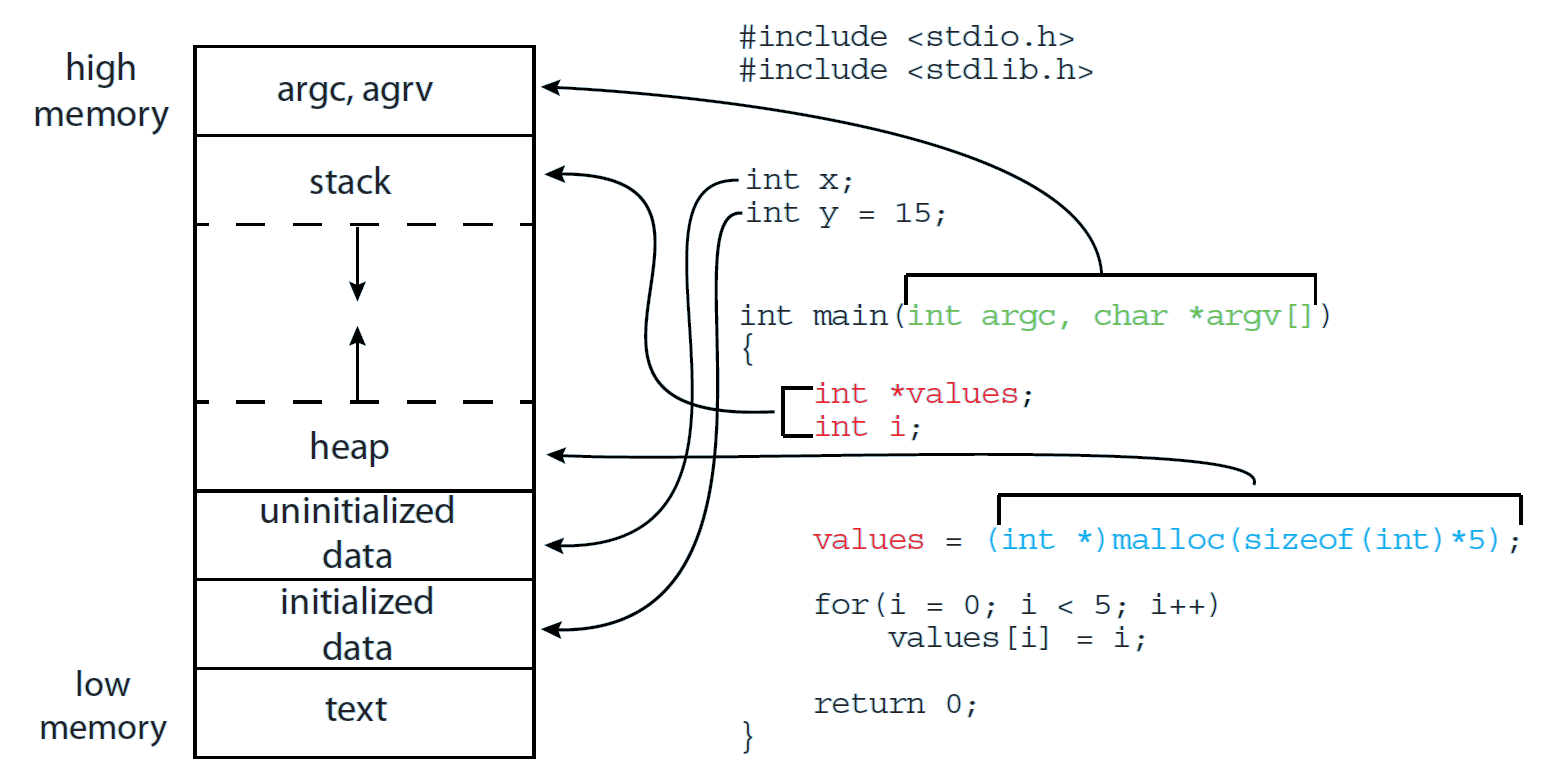
\includegraphics[keepaspectratio, width=12cm, height=9cm]{imagens/03/03 - Alocação de memória de um programa c.png}
\caption{Alocação de memória de um programa em C \\
Imagem retirada de: Silberschatz, A. Operating System Concepts, 10th,
página 108. \\}
\label{fig:Alocação de memória de um programa em C}
\end{figure}




Como a seção \texttt{text} e a \texttt{heap} crescem e diminuem
dinamicamente durante a execução do programa, existe um espaço, à ser
utilizado, entre ambos, de forma que a seção \texttt{stack}, sai de um
endereço superior da memória para um inferior, e o \texttt{heap} da
inferior para a superior. Na Figura \label{fig:Alocação de memória de um programa em C}, o endereço superior está chamado
de \emph{high-memory}, e o inferior de \emph{low-memory}. É papel do
sistema operacional de assegurar que ambas as seções não se sobreponham.

Cada processo é representado, no sistema operacional, pelo PCB
(\emph{Process Control Block}), uma lista encadeada contendo informações
como:

\begin{enumerate}
\def\labelenumi{\arabic{enumi}.}

\item
  \emph{Process state} - Podendo ser: \texttt{New}, \texttt{Running},
  \texttt{Waiting}, \texttt{Ready}, \texttt{Terminated}.
\item
  \emph{Program Counter} - Contador que indica o endereço da próxima
  instrução.
\item
  \emph{CPU registers} - Valor dos registradores da CPU.
\item
  \emph{CPU-scheduling information} - Informação sobre a prioridade do
  processo.
\item
  \emph{Memory-management information} - Informações sobre o
  gerenciamento de memória.
\item
  \emph{Accounting information} - Aqui está incluído dados como a
  quantidade de CPU usada.
\item
  \emph{I/O status information} - Informação sobre arquivos abertos,
  dispositivos I/O utilizados etc.
\end{enumerate}

\hypertarget{contexto-de-execuuxe7uxe3o}{%
\section{Contexto de Execução}\label{contexto-de-execuuxe7uxe3o}}

No código a seguir, temos a duas declarações da variável \texttt{a}.
Isso é possível pois cada declaração está dentro de um contexto de
execução diferente, de forma que cada função representa uma posição de
memória distinto, e, assim, seus conteúdos ocupam um espaço, ou
\texttt{Stack\ Frame}, específico da seção \texttt{stack}. Então, quando
uma função é chamada, o \texttt{Program\ Counter} é desviado para essa a
posição da memória, passando a executar as instruções lá inseridas, até
ser redirecionado de volta ao endereço inicial (no qual a função foi
chamada), descartando esse \texttt{Stack\ Frame}. O conteúdo contido no
\texttt{Stack\ Frame} descartado, não é removido da memória, por causa
do custo computacional de fazê-lo, fato gerador do chamado lixo de
memória (\texttt{Stack\ Frame} sem contexto), diminuindo, assim, o
\texttt{stack}. Quando um novo \texttt{Stack\ Frame} é concebido, esse
sobrescreve o lixo de memória anteriormente criado, aumentando o
\texttt{stack}.


\begin{minted}[mathescape, linenos]{c}

    void f()
    {
        int a = 4;
        printf("%d\n", a);
    }
    
    int main(int argc, char *argv[])
    {
        int a = 1;
        f();
        printf("%d\n", a);
    
    }

\end{minted}




Cada tipo de variável ocupa uma quantidade de bits específico, como
descriminado abaixo:

\begin{enumerate}
\def\labelenumi{\arabic{enumi}.}
\tightlist
\item
  \texttt{char:\ 8\ bits}
\item
  \texttt{int:\ 16\ bits}
\item
  \texttt{long:\ 32\ bits}
\item
  \texttt{float:\ 32\ bits}
\item
  \texttt{double:\ 64\ bits}
\end{enumerate}

\hypertarget{ponteiros}{%
\section{Ponteiros}\label{ponteiros}}

No programa mostrado na Figura \label{fig:Alocação de memória de um programa em C}, foi inicializada uma variável do typo
\texttt{int\ *}, o qual representa um ponteiro \texttt{int}. Os
ponteiros são baseados na ideia da indireção, ou seja, na referencia
indireta à outra posição da memória de tamanho \texttt{int} (16 bits).
Por ser uma referência, ele não ocupa o espaço referido, e sim um
específico para o seu tipo. No caso de uma arquitetura de 64 bits, o
ponteiro ocupa 8 bytes (64 bits).

O trecho de código da Figura \label{fig:Alocação de memória de um programa em C},


\begin{minted}[mathescape, linenos]{c}

    int *values;
    values = (int *) malloc(sizeof(int)*5);
    
    for(i = 0; i < 5; i++){
        values[i] = i; 
        // *(p + i) = i - Equivalente à: &values + i * sizeof(int) 
        // <= i
    }

\end{minted}


mostra que, o valor no qual está sendo referenciado pelo ponteiro
values, está no \texttt{heap} (jogado lá pela função \texttt{malloc(3)})
ocupando um espaço de 5 \texttt{int} (ou seja, 5 de 16 bits ou 80 bits).
Cada espaço desse é utilizado pela variável \texttt{i}, do tipo
\texttt{int}, fazendo, assim, com que o espaço referenciado por
\texttt{values} possa receber 5 do tipo \texttt{int}, como é utilizado
dentro do loop \texttt{for}, com a artimética de ocupação
\texttt{(\&values\ +\ i*sizeof(int))}, adicionado no código em forma de
cometário.

Podemos pensar na variável do ponteiro como um baú, no qual ao por
\texttt{*}, estamos acessando o conteúdo do baú, \texttt{\&} para o
endereço de memória que contém o valor referenciado,

No código a seguir, podemos ver 3 operações distintas com o ponteiro
\texttt{p}, as quais \texttt{\&} revela o endereço de memória do valor
``apontado'', \texttt{*} acessa o conteúdo da memória e, por fim,
\texttt{p} sem nenhum operador retorna o endereço da variável \texttt{p}
na \texttt{stack}.


\begin{minted}[mathescape, linenos]{c}

    int *values;
    int *p = malloc(sizeof(int)*4);
    
    p[0] = 10;
    printf("&p = %p/n", &p); // Endereço da referência (heap)
    printf("&p = %d/n", *p); // Conteúdo da referência
    printf("p = %p/n", p); // Endereço de p (Stack)

\end{minted}



%\hypertarget{aula-4}{%
%\chapter{Aula: 4}\label{aula-4}}




\hypertarget{processos-e-threads}{%
\chapter{Processos e threads}\label{processos-e-threads}}

\hypertarget{thread-uxe9-uma-parte-do-processo}{%
\subsection{Thread é uma parte do Processo}\label{thread-uxe9-uma-parte-do-processo}}

Como dito na aula anterior, um processo é uma entidade ativa a qual se
refere à um programa em execução. Porém, a CPU não recebe essa entidade
na sua integralidade para processamento, e sim uma parte da mesma
chamada de \emph{Thread} (a \emph{Thread} pode ser definida como uma
unidade de processamento do processo). Nessa está contido os elementos
necessários para a mudança de contexto da CPU (\emph{CPU Context
Switch}), como os valores dos registradores utilizados, a memória Stack
e o PC (\emph{Program Counter}).

Em sistemas \emph{single-threaded} (única \emph{thread} por processo,
normalmente encontrado em sistemas mais antigos), cada nova tarefa a ser
executada deve-se passar pela criação de um novo processo.

\hypertarget{concurrency-vs-parallelism}{%
\subsection{Concurrency vs Parallelism}\label{concurrency-vs-parallelism}}

Uma observação importante é que um programa, em um sistema com um único
núcleo de processamento, pode rodar em simultâneo (\emph{concurrency})
com outros programas, devido a alternação do processo a ser executado
pela CPU em certos períodos de tempo, porém não em paralelo
(\emph{parallelism}), por não ter múltiplos núcleos.

\hypertarget{concurrency}{%
\subsection{Concurrency}\label{concurrency}}

Os processos são distribuídos para a CPU com a técnica
\emph{Round-Robin}, com a qual é gerada uma fila de processos, e a saída
de cada fila vai para o processador. Após um certo período de tempo,
esse processamento é interrompido, o seu contexto é salvo, e o processo
volta para o final da fila (observar que há políticas de prioridades. No
exemplo está sendo considerado que todos os processos têm a mesma
prioridade). Um novo processo então é chamado para execução, com o seu
contexto de CPU sendo carregado. Essa mudança de contexto da CPU
(\emph{CPU context-switch}) é o que torna possível a CPU retomar o
processamento de um processo específico do momento que o mesmo foi
anteriormente interrompido. Esse ciclo continua até a conclusão de todos
os processos.

\hypertarget{criauxe7uxe3o-de-novos-processos}{%
\subsection{Criação de novos processos}\label{criauxe7uxe3o-de-novos-processos}}

Na linguagem C, a criação de um novo processo passa pela função
\texttt{clone(2)}, a qual copia, conforme instruções do programador,
todos os elementos do processo original para o novo processo,
consumindo, assim, recursos como a memória, com a locação múltipla dos
mesmos dados. Uma tentativa de otimização pode ser observada na função
\texttt{fork(2)} (que é uma implementação específica da função
\texttt{clone(2)}), que utiliza o conceito de \texttt{CoW} (\emph{Copy
on Write}, ou cópia na escrita, que é uma funcionalidade do sistema de
gerenciamento de memória), somente copiando os dados, para o novo
endereço de memória, caso haja alteração dos mesmos. Isso é possível com
o uso dos ponteiros, discutidos na aula anterior, para a leitura dos
dados. É importante notar que a execução do processo criado continuará a
partir da última posição do IP (\emph{Instruction Pointer}, ou ponteiro
de instrução), fazendo com que as instruções escritas antes do
\texttt{clone(2)} ou \texttt{fork(2)} nunca sejam lidas.

A função \texttt{fork()} retorna:

\begin{enumerate}
\def\labelenumi{\arabic{enumi}.}

\item
  -1, caso tenha falhado;
\item
  0, para o processo filho, com o PPID (\emph{Parent Process
  Identifier}, ou identificador do processo pai) equivalendo ao PID
  (\emph{Process Identifier}, ou identificador do processo) do processo
  pai
\item
  PID do processo filho, no processo pai.
\end{enumerate}


\begin{minted}[mathescape, linenos]{c}

    #include <stdio.h>
    #include <sys/types.h>
    #include <unistd.h>
    
    int main()
    {
            printf("Before fork: %d \n", getpid());
            pid_t returned = fork(void);
            
            if(returned == 0){
                    printf("Child here: %d \n", getpid());
            } else {
                    printf("Parent here: %d, child pid: %d \n", getpid(), returned);
            }
            
            return 0;
    }

\end{minted}



\hypertarget{por-que-devemos-criar-novos-processos}{%
\subsection{Por que devemos criar novos processos?}\label{por-que-devemos-criar-novos-processos}}

Há dois motivos para a criação de novos processos (em sistemas mais
antigos):

\begin{enumerate}
\def\labelenumi{\arabic{enumi}.}
\tightlist
\item
  Inicialização de um novo programa, com o \texttt{execve(2)}.
\item
  Múltiplas tarefas de um mesmo programa.
\end{enumerate}

Apesar da otimização citada na seção anterior (com o \texttt{CoW}), o
procedimento de criação de um novo processo é custoso de recursos
computacionais, sendo o \emph{multi-threading} (múltiplas threads no
mesmo processo) uma solução para a criação de múltiplas tarefas de um
mesmo programa (caso 2).

\hypertarget{execve2}{%
\subsection{execve(2)}\label{execve2}}

A função \texttt{execve(2)} tem como objetivo alterar a imagem de
execução, que está contida no processo, para a do novo programa, isso é,
o \emph{Data}, \emph{Heap}, \emph{Stack} e \emph{Text} serão carregados
com o conteúdo do novo programa.

A execução do programa \texttt{hello.c}, dentro do \texttt{execv.c},
ambos escritos abaixo, retornará o mesmo \texttt{pid} (\emph{Process
Identification}) do que no primeiro programa, pois o processo é o mesmo,
mas a imagem é diferente.

Arquivo \texttt{execv.c}:


\begin{minted}[mathescape, linenos]{c}


    #include <stdio.h>
    #include <sys/types.h>
    #include <unistd.h>
    
    int main()
    {
            char *argv[] = {"", NULL}; //array of char*
            char *envp[] = {"", NULL}; //array of char*
            
            printf("before execve. pid(%d)\n", getpid());
            
            //Troca a imagem de execução.
            int ret = execve("hello", argv, envp); 
            //Caso positivo, as linhas a seguir não existirão mais;
            
        printf("supposed never executed\n");
            if(ret == -1) {
                    perror("execve failed");
                    return 1;
            }
            
            return 0;
    }

\end{minted}

Arquivo \texttt{hello.c}:


\begin{minted}[mathescape, linenos]{c}


    #include <stdio.h>
    #include <sys/types.h>
    #include <unistd.h>
    
    int main()
    {
            printf("hello world from pid(%d)\n", getpid());
            return 0;
    }

\end{minted}



*Obs: o programa irá buscar um arquivo em código de máquina, e não em C.
Assim:

\begin{lstlisting}[language=bash]
    $ make hello.c
    $ make execv && ./execv
\end{lstlisting}


\hypertarget{multi-threading}{%
\subsection{Multi-threading}\label{multi-threading}}

É importante notar que os sistemas operacionais evoluíram, com os mais
antigos limitando-se à \emph{single-threading} (uma \emph{thread} por
processo), e os mais novos rompendo essa limitação, passando à
\emph{multi-threading} (múltiplas \emph{threads} por processo), como
mostrado na Figura \ref{fig:imagens/04/04 - single-multi-threaded.png}.


\begin{figure}[h!]
\centering
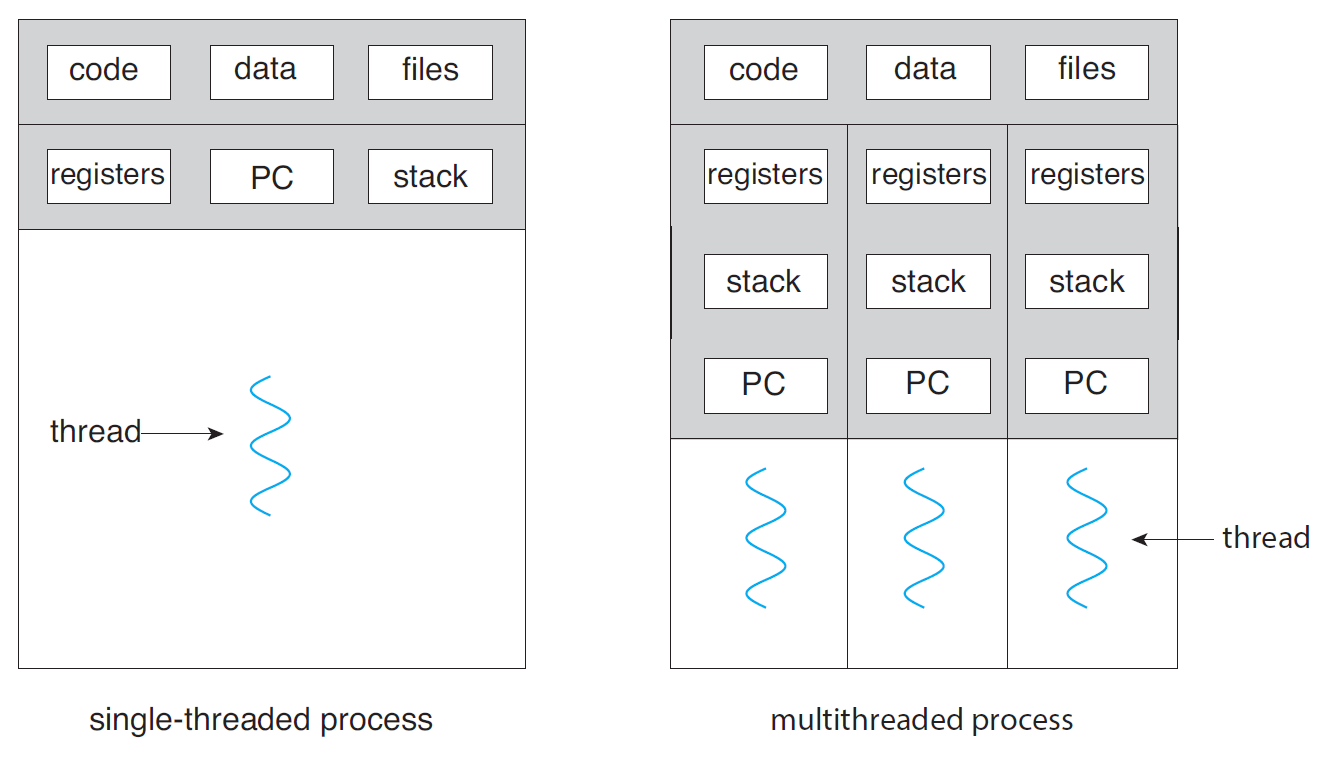
\includegraphics[keepaspectratio, width=12cm, height=9cm]{imagens/04/04 - single-multi-threaded.png}
\caption{Single and Multi-Threaded Example \\
Imagem retirada de: Silberschatz, A. Operating System Concepts, 10th,
página 160. \\}
\label{fig:imagens/04/04 - single-multi-threaded.png}
\end{figure}



O \emph{multi-threading} trás consigo diversas vantagens, como:

\begin{enumerate}
\def\labelenumi{\arabic{enumi}.}
\tightlist
\item
  Responsividade: Um programa continua rodando mesmo quando uma parte
  sua é bloqueada, trava ou demora para concluir.
\item
  Compartilhamento de Recursos: As \emph{Threads} compartilham o mesmo
  código e dados por padrão.
\item
  Economia: é mais econômico criar uma \emph{Thread} do que um processo.
  É mais rápido trocar o contexto da CPU (\emph{CPU context-switch})
  entre \emph{Threads} do que entre processos, desde que estejam em
  \emph{userspace}.
\item
  Escalabilidade: \emph{Threads} podem usufruir do paralelismo, rodando
  em múltiplas CPU's em simultâneo de forma assíncrona.
\end{enumerate}

É com o \emph{multi-threading} que um programa consegue tirar vantagem
de vários núcleos de processamento, de forma a utilizar tanto o
\emph{Concurrency} como o \emph{Parallelism} (multiplas \emph{threads}
com um único núcleo ocorre o \emph{Concurrency} mas não o
\emph{Parallelism}).

\hypertarget{funuxe7uxe3o-como-argumento-de-outra-funuxe7uxe3o.}{%
\section{Função como argumento de outra função.}\label{funuxe7uxe3o-como-argumento-de-outra-funuxe7uxe3o.}}

Utilizando Ponteiros, podemos passar uma função como argumento de outra
função, basta coletar o endereço de memória da mesma (o nome da função
coincide com o endereço dela) e passar para um ponteiro. Depois passar o
ponteiro no argumento da função. A seguir temos um código de exemplo de
como utilizar ponteiros para funções (bastando passar a variável
\texttt{fp} como argumento de uma função).



\begin{minted}[mathescape, linenos]{c}

    int funca(int); //declarando uma função sem definir
    int funcb(int);
    
    int main()
    {
            int (*fp)(int); 
            //Declarando um ponteiro de função com um argumento int
            
            fp = funca;// fp = funcb;
            printf("fp(%d) = %d\n", 3, fp(3));
    }
    
    int funca(int n)
    {
            return 2 * n
    }
    
    int funcb(int n)
    {
            return 100 * n
    }
\end{minted}



\hypertarget{complementar}{%
\section{Complementar}\label{complementar}}

\hypertarget{pesquisar-sobre}{%
\subsubsection{Pesquisar Sobre}\label{pesquisar-sobre}}

Para saber mais, procurar sobre as funções do bash \$:

\begin{enumerate}
\def\labelenumi{\arabic{enumi}.}
\tightlist
\item
  ps aux
\item
  ps aux \textbar{} wc -l
\item
  ps -ef
\item
  top (u)
\item
  htop
\item
  lscpu
\end{enumerate}

Função \texttt{C}: 1. atoi() -\textgreater{} alphabet to integer 7.

%\hypertarget{aula-5}{%
%\chapter{Aula: 5}\label{aula-5}}




\hypertarget{retomando-aos-processos}{%
\chapter{Retomando aos processos}\label{retomando-aos-processos}}

Nas últimas, foram debatidos diversos aspectos dos processos dos SO
(Sistemas Operacionais). Esses aspectos orbitam os 3 pontos enfatizado a
seguir:

\begin{enumerate}
\def\labelenumi{\arabic{enumi}.}

\item
  Identificar os componentes de um processo.
\item
  Criação e Término de processos
\item
  Comunicação entre processos: \emph{Shared Memory} x \emph{Message
  Passing}.
\end{enumerate}

\hypertarget{componentes-de-um-processo.}{%
\subsection{Componentes de um
processo.}\label{componentes-de-um-processo.}}

Enquanto que um programa é uma entidade passiva localizada na memória
secundária, um processo é instância ativa de um programa, e está
localizado na memória principal em quatro sessões básicas (Como mostrado
na Figura \ref{fig:Processo na memória principal }): \emph{Text}, código executável; \emph{Data}, variáveis globais; \emph{Heap}, memória dinamicamente alocada; \emph{Stack},
armazenamento de dados temporários.



\begin{figure}[h!]
\centering
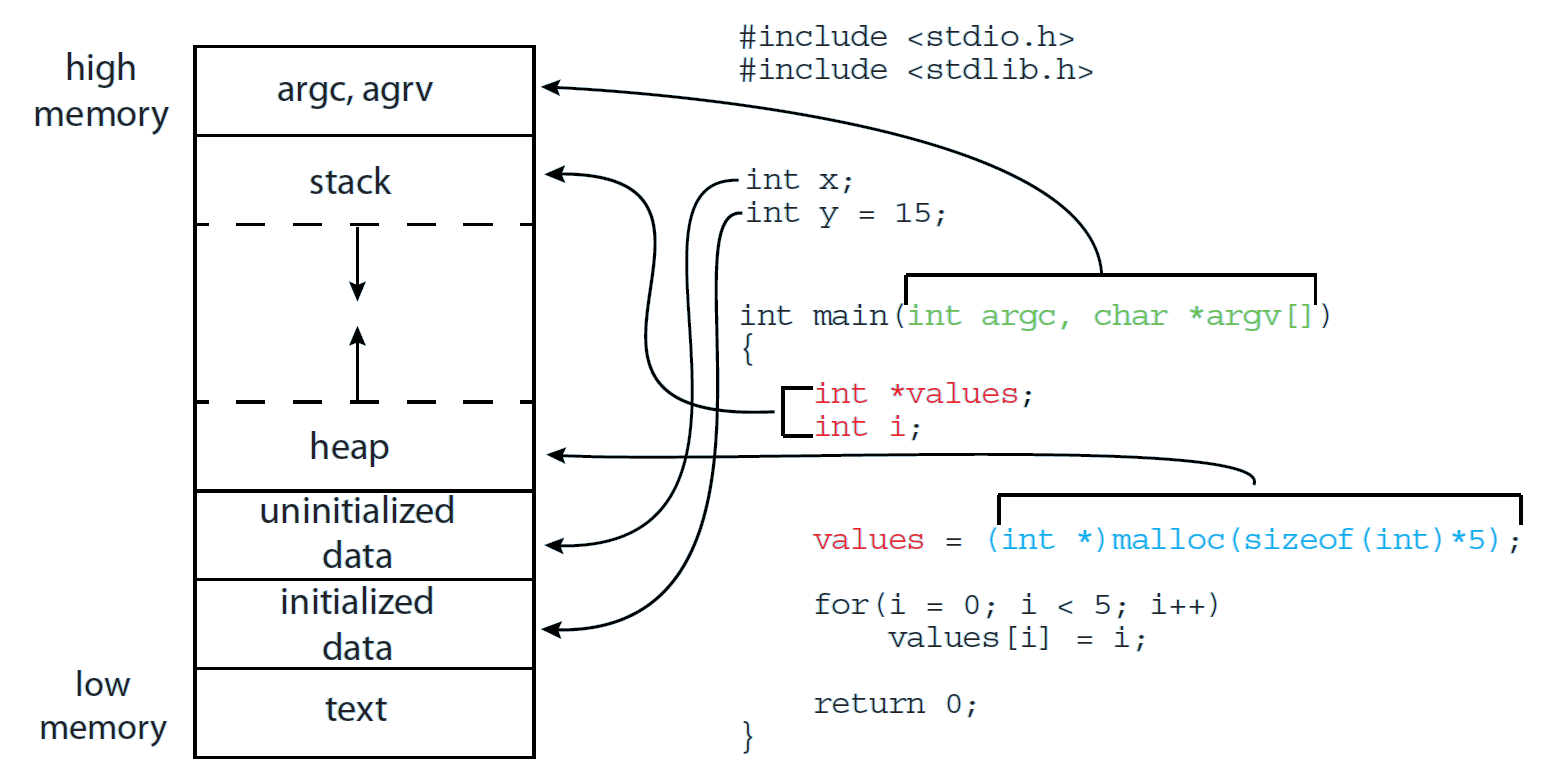
\includegraphics[keepaspectratio, width=12cm, height=9cm]{imagens/03/03 - Alocação de memória de um programa c.png}
\caption{Processo na memória principal \\
Imagem retirada de: Silberschatz, A. Operating System Concepts, 10th,
página 106. \\}
\label{fig:Processo na memória principal}
\end{figure}

Do ponto de vista do Sistema Operacional, cada processo é representado
pelo \emph{Process Control Block} (PCB), mostrado na Figura \ref{fig:PCB: Representação do processo no SO}, o qual
contém vários pedaços de informação necessários para iniciar ou
reiniciar um processo específico, como \emph{Process State},
\emph{Program counter}, \emph{CPU registers} e \emph{CPU-scheduling
information}.

\begin{figure}[h!]
\centering
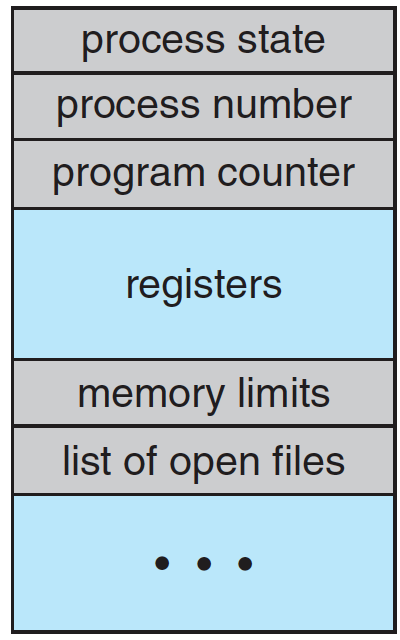
\includegraphics[keepaspectratio, width=12cm, height=9cm]{imagens/05/05 - Process Block Control (PCB).png}
\caption{PCB: Representação do processo no SO   \\
Imagem retirada de: Silberschatz, A. Operating System Concepts, 10th,
página 109 \\}
\label{fig:PCB: Representação do processo no SO}
\end{figure}



De forma geral, os processos podem assumir 5 estados (Como mostrado na
Figura \ref{fig:Estados de um process}): criado, pronto, rodando, esperando e terminado.


\begin{figure}[h!]
\centering
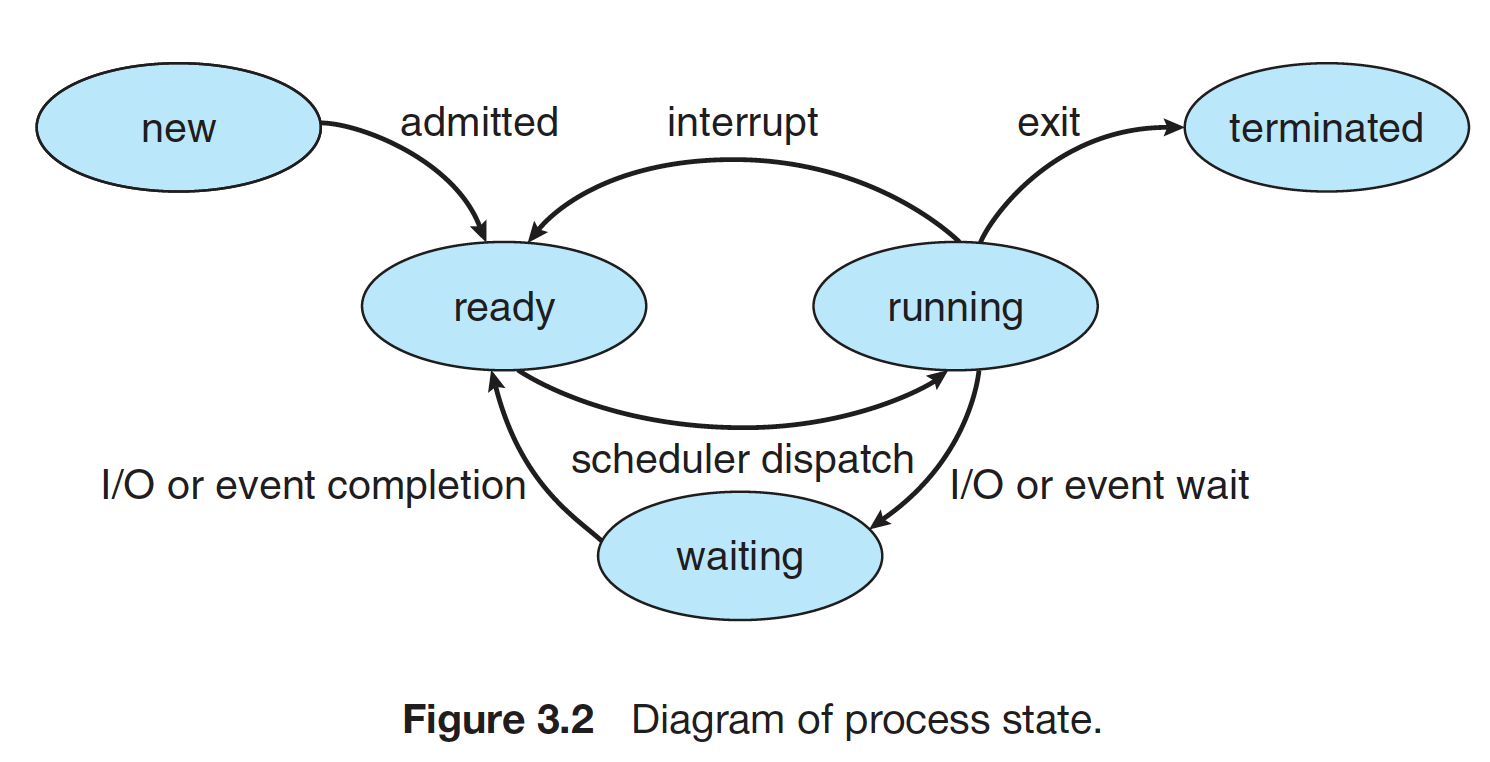
\includegraphics[keepaspectratio, width=12cm, height=9cm]{imagens/05/05 - Diagram of Process State.png}
\caption{Estados de um processo   \\
Imagem retirada de: Silberschatz, A. Operating System Concepts, 10th,
página 109. \\}
\label{fig:Estados de um process}
\end{figure}


No Linux, todos os PCB's encontram-se em uma lista duplamente encadeada
(com o próximo e o anterior), com o sistema operacional armazenando um
ponteiro para a estrutura que está atualmente em execução pela CPU.
Mostrado na Figura \ref{fig:Representação da fila encadeada}.


\begin{figure}[H]
\centering
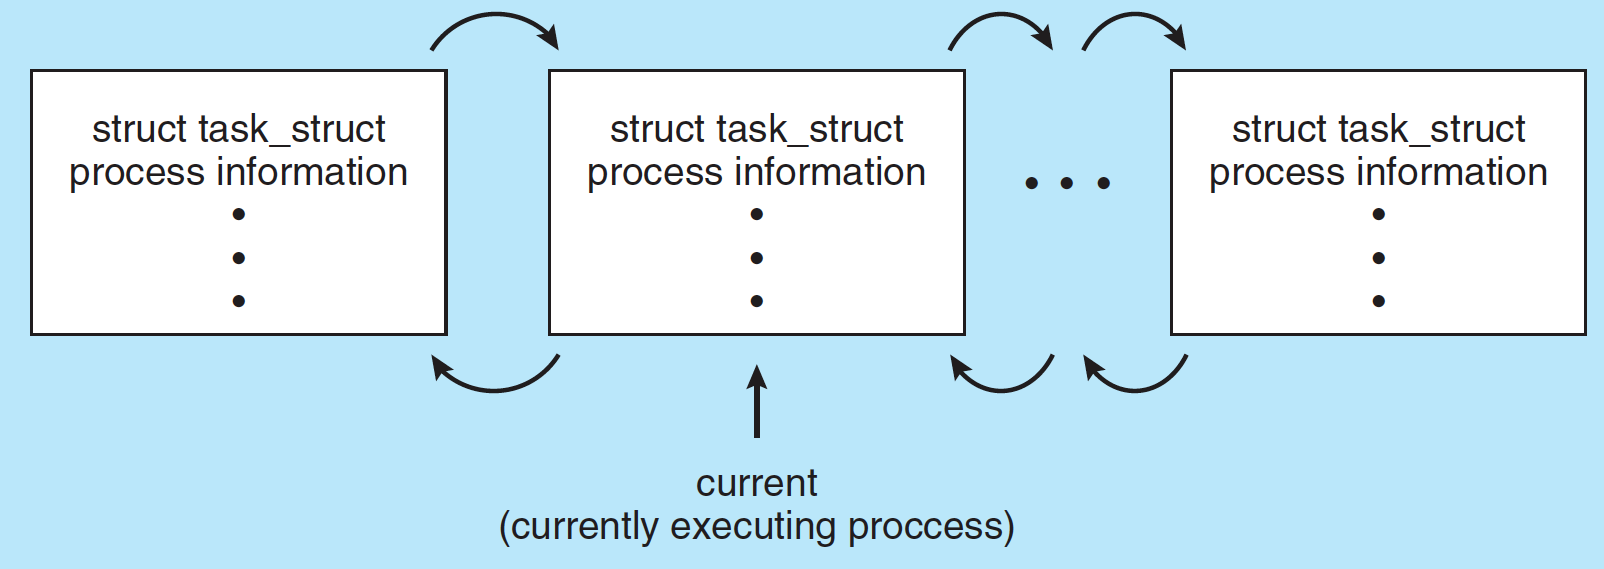
\includegraphics[keepaspectratio, width=12cm, height=9cm]{imagens/05/05 - Representacao da fila encadeada.png}
\caption{Representação da fila encadeada   \\
Imagem retirada de: Silberschatz, A. Operating System Concepts, 10th,
página 111. \\}
\label{fig:Representação da fila encadeada}
\end{figure}



Conforme o estado do processo muda, o PCB também muda de fila,
alternando entre a fila encadeada de ``pronto'' (pronto para ser
executado) e espera (espera de ocorrência de evento), mostradas na
Figura \ref{fig:Filas de espera e pronto}.

\begin{figure}[h!]
\centering
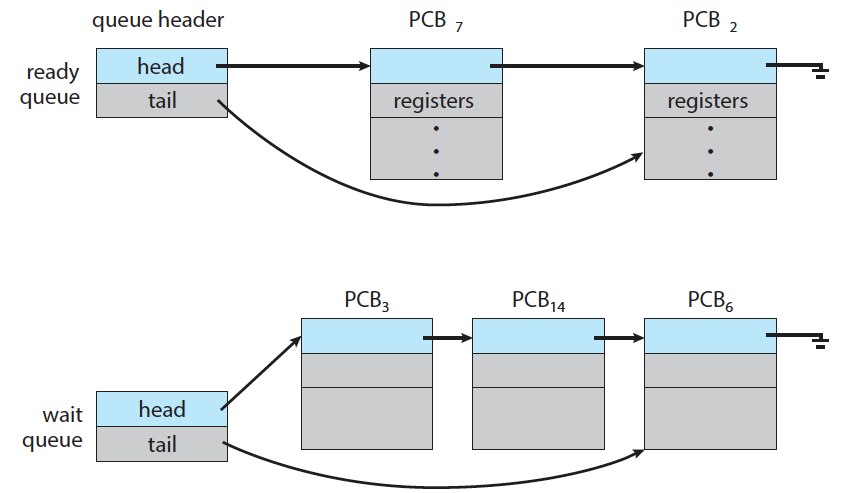
\includegraphics[keepaspectratio, width=12cm, height=9cm]{imagens/05/05 - Filas de espera e pronto.png}
\caption{Filas de espera e pronto   \\
Imagem retirada de: Silberschatz, A. Operating System Concepts, 10th,
página 112. \\}
\label{fig:Filas de espera e pronto}
\end{figure}



O responsável por depositar e recolher os PCB's dessas filas é o
\emph{process Scheduling}, o qual foi representado no diagrama da Figura
\ref{fig:Diagrama de agendamento de processos}.


\begin{figure}[h!]
\centering
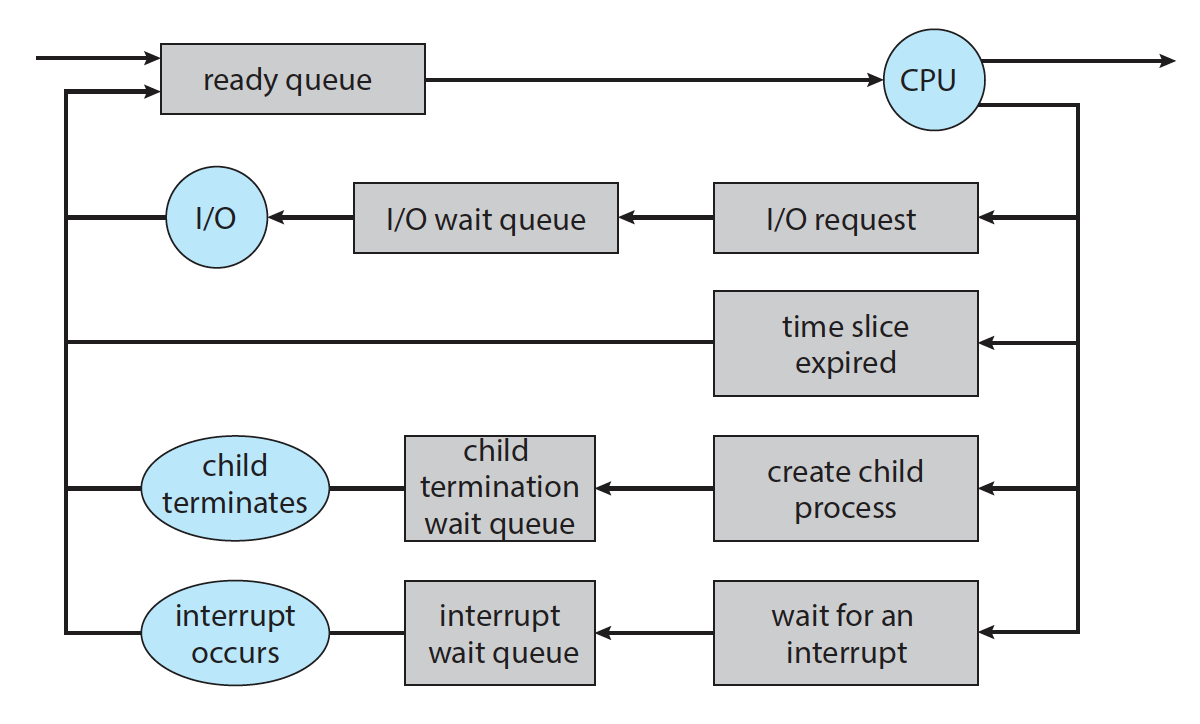
\includegraphics[width=12cm, height=9cm]{imagens/05/05 - Diagrama Agendamento de Processos.png}
\caption{Diagrama de agendamento de processos   \\
Imagem retirada de: Silberschatz, A. Operating System Concepts, 10th,
página 113. \\}
\label{fig:Diagrama de agendamento de processos}
\end{figure}


O \emph{CPU Scheduling}, por sua vez, tem como papel recolher um
processo da fila \emph{ready} para um núcleo de processamento. Para ser
alocado na CPU, é necessário salvar o estado do processo anteriormente
alocado, bem como os elementos necessários para continuar processando-o
posteriormente, e carregar o novo contexto de execução. No decorrer
dessa tarefa, chamada de \emph{Context Switch}, a CPU fica ociosa, como
mostra a Figura \ref{fig:Diagrama da troca de contexto}.

\begin{figure}[h]
\centering
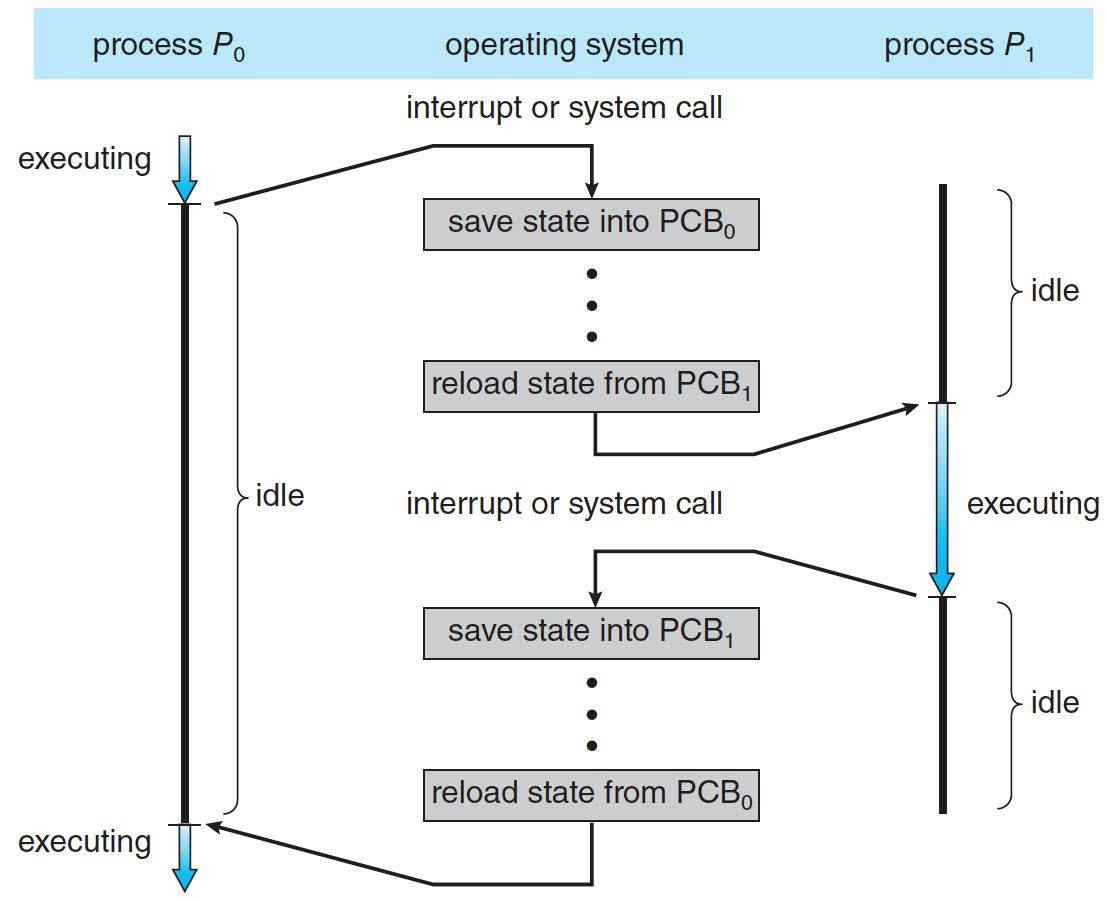
\includegraphics[keepaspectratio, width=12cm, height=9cm]{imagens/05/05 - Diagrama Contex Switch.png}
\caption{Diagrama da troca de contexto   \\
Imagem retirada de: Silberschatz, A. Operating System Concepts, 10th,
página 113. \\}
\label{fig:Diagrama da troca de contexto}
\end{figure}


\hypertarget{criauxe7uxe3o-e-tuxe9rmino-de-um-processo.}{%
\subsection{Criação e Término de um
processo.}\label{criauxe7uxe3o-e-tuxe9rmino-de-um-processo.}}

Cada processo tem uma identificação única chamada de \texttt{pid}
(\emph{process identifier}). A partir dele pode ser criado um processo
filho. Conscutivas criações formam uma árvore de processos, mostrada na
Figura \ref{fig:Árvore de processos típico de sistema Linux}.


\begin{figure}[H]
\centering
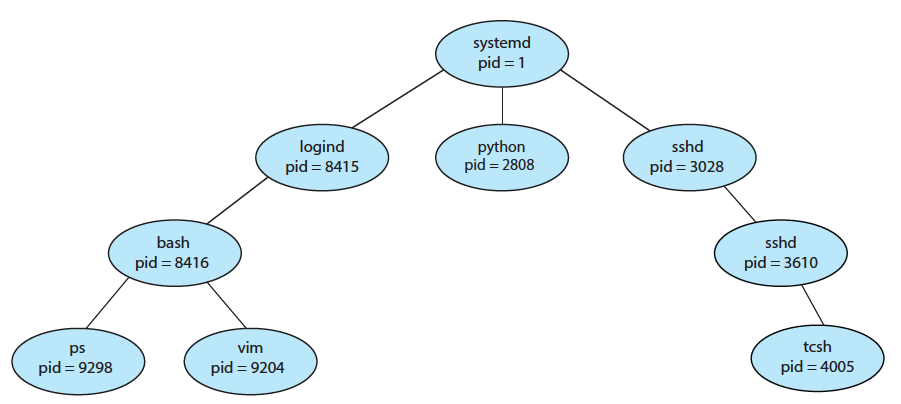
\includegraphics[width=8cm, height=5cm]{imagens/05/05 - Arvore de processos em um sistema linux.png}
\caption{Árvore de processos típico de sistema Linux   \\
Imagem retirada de: Silberschatz, A. Operating System Concepts, 10th,
página 116. \\}
\label{fig:Árvore de processos típico de sistema Linux}
\end{figure}


O ciclo de criação e término de um processo, mostrado na Figura \ref{fig:Criação e término de um processo}, passa
pelas funções de chamada de sistema na linguagem \texttt{C}:
\texttt{fork()}, para criar um novo processo; \texttt{wait()}, esperar o
processo filho acabar; \texttt{execve()}, troca a imagem de execução
(troca o programa); \texttt{exit()}, encerrar o processo.


\begin{figure}[h!]
\centering
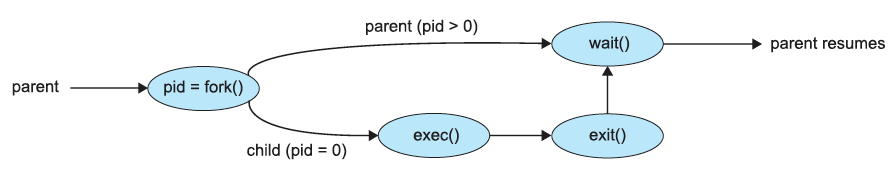
\includegraphics[keepaspectratio, width=15cm, height=17cm]{imagens/05/05 - Process Creation.png}
\caption{Criação e término de um processo   \\
Imagem retirada de: Silberschatz, A. Operating System Concepts, 10th,
página 119. \\}
\label{fig:Criação e término de um processo}
\end{figure}


Alguns sistemas não permitem que um processo ``viva'' sem que o ``pai''
exista. Então, se o ``pai'' for encerrado, todos os ``filhos'' serão
encerrados. Da mesma forma que os filhos dos filhos. Fenômeno chamado de
\emph{cascading termination}

Ao chamar a função \texttt{exit()}, um processo filho tem seus recursos
deslocados pelo sistema operacional. Porém ele continua na tabela de
processos até o processo pai executar a função \texttt{wait()}, pois
nessa tabela está contido o estado de saída do mesmo. Durante essa
transição, de seus recursos terem sido deslocados mas ainda estar na
tabela de processos, o processo é chamado de \texttt{Zumbie}, o que,
normalmente, ocorre para todos os processos (ao serem terminados) por um
curto período de tempo. Se o pai não chamar a função \texttt{wait()} e
terminar sua execução, os processos filhos passarão a ser chamados de
processos \texttt{órfãos}. O Sistema Operacional Linux utiliza de outros
processos para herdar os \texttt{órfãos} e libera-los da tabela de
processos chamando a função \texttt{wait()}.

\hypertarget{comunicauxe7uxe3o-entre-processos-shared-memory-x-message-passing.}{%
\section{\texorpdfstring{Comunicação entre processos: \emph{Shared
Memory} x \emph{Message
Passing}.}{Comunicação entre processos: Shared Memory x Message Passing.}}\label{comunicauxe7uxe3o-entre-processos-shared-memory-x-message-passing.}}

Um processo pode ter sido criado com o objetivo de executar um algoritmo
que independe de outros processos (esse processo é chamado de
independente). Ou, pode ter sido criado para cooperar com outros
processos (esse processo é chamado de cooperativo). Para que a
cooperação ocorra, é necessário criar um canal de comunicação (um
\emph{Interprocess Communication - IPC} ), de tal maneira que os dados
possam ser transmitidos de uma para outra. Há dois métodos para tal: o
\emph{Shared Memory} (compartilhamento de memória); e o \emph{Message
Passing} (sistema de passagem de mensagem).

Há várias razões para ter um processo cooperativo. 1. Troca de
informações: Compartilhamento de informações entre os interessados. 2.
Aceleração computacional: Dividir uma tarefa em várias pequenas partes
e, assim, processá-los ao mesmo tempo. 3. Modularidade: Com as funções
do sistema dividido em diferentes processos ou threads.

\hypertarget{shared-memory}{%
\subsection{Shared Memory}\label{shared-memory}}

\emph{Shared Memory} é o método que torna uma faixa de endereços de
memória acessível à diferentes processos. Por questões de segurança, o
sistema operacional (de forma padrão) não permite que os processos
tenham acesso aos espaços de memória dos outros. Para que esse método
ocorra, é fundamental que todos os processos participantes desse método
concordem em compartilhar a sua faixa de memória. Após executado, o
sistema operacional não mais intervem, deixando para os processos a
responsabilidade de garantir que não ocorra o problema chamado
\emph{Race Conditions} (ou condição de disputa).

O \emph{Race Conditions} decorre de um problema de \emph{concurrency}
(simultaneidade) entre os diferentes processos, como a escrita em um
mesmo endereço de memória transcorrendo por mais de um processo ao mesmo
tempo.

Uma solução para garantir a comunicação entre os processos é utilizando
a arquitetura \emph{producer-consumer}, no qual o processo
\emph{producer} produz e armazena o conteúdo em um buffer, que será
consumido pelo \emph{consumer} posteriormente. Esse \emph{buffer} pode
ser \emph{unbounded buffer} (não tem limites de tamanho) ou
\emph{bounded buffer} (com o tamanho limitado).

\hypertarget{message-passing}{%
\subsection{Message Passing}\label{message-passing}}

A idéia por de trás do método \emph{message passing} é a de passar a
responsabilidade da distribuição e validade da comunicação
inter-processual para o sistema operacional, promovendo uma abstração de
uso facilitado (em comparação ao \emph{shared memory}), pois descarta a
necessidade da criação explícita de um código de gerenciamento de acesso
e manupulação dos dados compartilhados. Esse mecanismo de comunicação
cria um elo de ligação (\emph{link}) entre dois processos, que demanda
ao menos duas operações: \emph{send(message)}; e
\emph{receive(message)}.

A implementação desse método passa por 3 pontos:

\begin{enumerate}
\def\labelenumi{\arabic{enumi}.}
\tightlist
\item
  Comunicação direta e indireta.
\item
  Síncrona ou assíncrona.
\item
  \emph{Buffer} automático ou explícito.
\end{enumerate}

\hypertarget{comunicauxe7uxe3o-direta}{%
\subsubsection{Comunicação Direta}\label{comunicauxe7uxe3o-direta}}

Na comunicação direta, o processo deve nomear explicitamente o nome do
receptor ou emissor: 1. \emph{send(P, message)}: Enviar menssagem para o
processo P 2. \emph{receive(Q, message)}: Receber mensagem do processo Q

\hypertarget{comunicauxe7uxe3o-indireta}{%
\subsubsection{Comunicação indireta}\label{comunicauxe7uxe3o-indireta}}

Na comunicação indireta, as mensagens passam através de uma abstração de
caixa de correios (\emph{mailbox} ou \emph{ports}) compartilhada, na
qual as mensagens podem ser postadas e removidas. Cada \emph{mailbox}
tem uma identificação única (no POSIX, cada \emph{mailbox} é
identificado por um inteiro). Nessa implementação, o processo deve
nomear de qual e para qual caixa de correios deve enviar ou receber a
mensagem:

\begin{enumerate}
\def\labelenumi{\arabic{enumi}.}
\tightlist
\item
  \emph{send(A, message)}: Enviar uma mensagem para o \emph{mailbox} A.
\item
  \emph{receive(A, message)}: Receber uma mensagem do \emph{mailbox} A.
\end{enumerate}

Um possível \emph{Race Condition} ocorre quando o processo P1 envia uma
mensagem, e o P2 e P3 estão chamando a função \texttt{receive()}. Para
evitar que isso aconteça, existem 3 possibilidades:

\begin{enumerate}
\def\labelenumi{\arabic{enumi}.}
\tightlist
\item
  Permitir que somente 2 processos estejam associados à uma caixa de
  correios.
\item
  Permitir que somente 1 processo por vez execute a função
  \texttt{receive()}
\item
  Permitir que o sistema operacional escolha qual processo deve receber
  (P1 ou P2, mas não ambos).
\end{enumerate}

\hypertarget{sincronia}{%
\subsubsection{Sincronia}\label{sincronia}}

Para cada um dos dois primitivos (\texttt{send()} e \texttt{receive()}),
o sistema de transmissão de mensagens pode assumir 2 estados, o síncrono
e o assíncrono:

\begin{enumerate}
\def\labelenumi{\arabic{enumi}.}
\item
  Síncrono (\emph{Blocking} ou bloqueante): 1.1. O emissor (P1) é
  travado até o receptor (P2) receber a mensagem. 1.2. O receptor (P1) é
  travado até uma mensagem ficar disponível.
\item
  Assíncrono (\emph{Nonblocking} ou não-bloqueante) 2.1. O emissor (P1)
  continua a executar suas instruções após a emissão da mensagem. 2.2. O
  receptor (P2) pode receber uma mensagem inválida (NULL), assim
  continuar sua execução mesmo sem ter recebido uma mensagem válida.
\end{enumerate}

\hypertarget{buffer}{%
\subsection{Buffer}\label{buffer}}

Todas as mensagens enviadas devem passar por um sistema de fila que,
basicamente, tem 3 formas distintas (que apenas variam sua capacidade):

\begin{enumerate}
\def\labelenumi{\arabic{enumi}.}
\tightlist
\item
  Capacidade 0 (\emph{Zero capacity} ou sem \emph{buffer}): O emissor
  deve ser síncrono com o receptor, caso contrário a mensagem será
  perdida.
\item
  Capacidade limitada (\emph{Bounded capacity}): O emissor pode ser
  assíncrono caso haja capacidade de armazenamento de mensagens no
  \emph{buffer}. E, caso a fila esteja cheia, deve ser bloqueado até
  haver espaço disponível.
\item
  Capacidade ilimitada (\emph{Unbounded capacity}): O emissor nunca é
  bloqueado, pois a fila não tem limites de recepção de mensagens.
\end{enumerate}

\hypertarget{complementar-1}{%
\section{Complementar}\label{complementar-1}}

Essa sessão faz alusão à outros conteúdos também importantes
relacionados com a aula, mas que dará ao leitor o papel de buscar mais
informações sobre os mesmos conforme sua necessidade e interesse.

\hypertarget{threads---criauxe7uxe3o-em-c}{%
\subsection{\texorpdfstring{Threads - criação em
\texttt{C}}{Threads - criação em C}}\label{threads---criauxe7uxe3o-em-c}}

Nas aulas anteriores foram discutidos as vantagens das threads em
comparação aos processos. Abaixo está um código comentado em \texttt{C}
para criação de threads.

\begin{minted}[mathescape, linenos]{c}

    #include <stdio.h>
    #include <pthread.h> //POSIX thread library, or pthread.
    
    
    int sum;
    void *runner(void *param);
    
    int main(int argc, char *argv[])
    {
            pthread_t tid;
            pthread_attr_t attr;
            
            pthread_attr_init(&attr); 
            //Atributo necessário para a criação da thread
            
            /*
             * pthread_create
             * tid vai retornar o 'id' da thread. 
             * runner é a função que será executada
             * argv[1] é o argumento no qual será passado para a função runner
             *
             */
            pthread_create(&tid, &attr, runner, argv[1]); 
            pthread_join(tid, NULL); //Espera uma thread Terminar
            
            return 0;
    }
    
    void *runner(void *param){
            
            int upper = atoi(param);
            int sum = 0;
            
            for(int i = 0; i < upper; i++){
                   sum += 1;
            }
            
            pthread_exit(0);
    }
\end{minted}



\hypertarget{pesquisar-sobre-1}{%
\subsection{Pesquisar Sobre}\label{pesquisar-sobre-1}}

\begin{enumerate}
\def\labelenumi{\arabic{enumi}.}

\item
  Teoria de filas
\item
  \emph{pipes} (mecanismo \emph{IPC - InterProcess Communication}) -
  Página 139 (Capítulo 3.7) de Silberschatz, A. Operating System
  Concepts, 10th.
\end{enumerate}


%\hypertarget{aula-6}{%
%\chapter{Aula: 6}\label{aula-6}}





\hypertarget{Introdução.}{%
\chapter{Retomando às Threads.}\label{Retomando às Threads.}}




Imagine, caro leitor, que você seja dono de uma loja e que você não
tenha funcionários, como na Figura \ref{fig:Loja de único atendente}. Todas as tarefas, entre
administrar o estoque, dar baixa no caixa e atender os clientes, deve
ser feito por você. Qual estratégia você deve tomar para tornar isso
possível ?

\begin{figure}[h!]
\centering
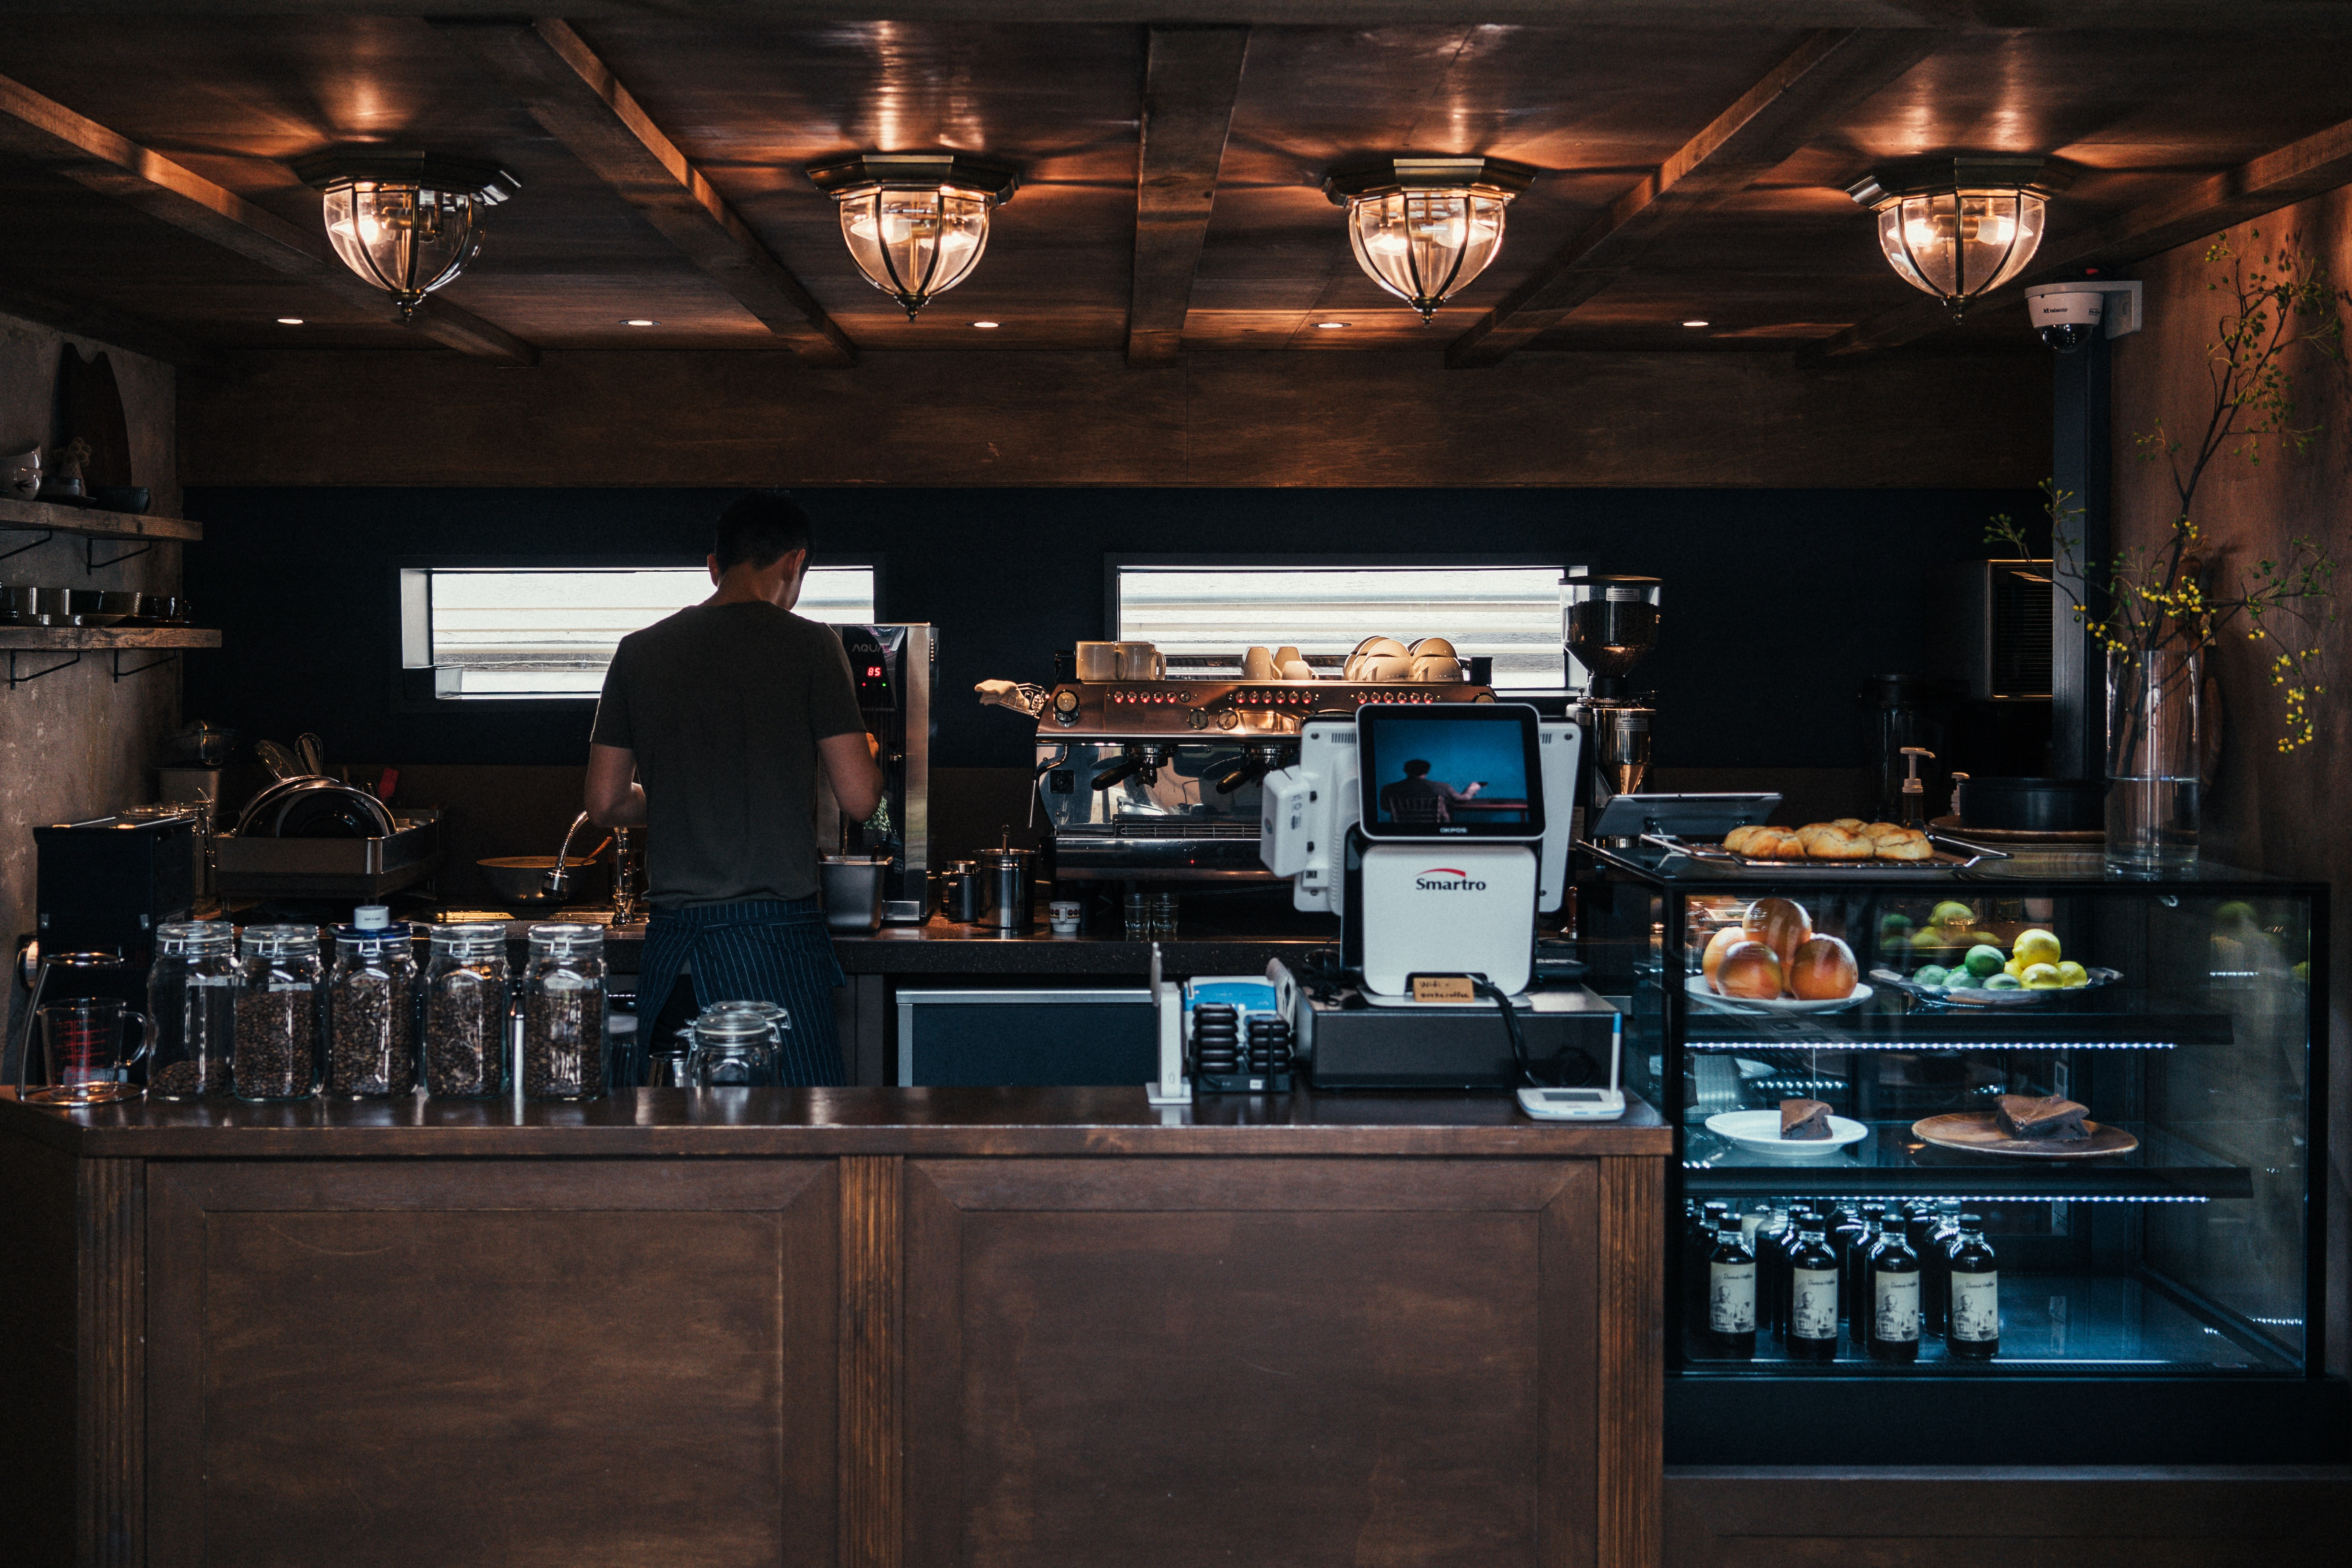
\includegraphics[keepaspectratio, width=12cm, height=9cm]{imagens/06/06 - single worker store.jpg}
\caption{Loja de único atendente   \\
Autor: rawkkim, de: unsplash.com \\}
\label{fig:Loja de único atendente}
\end{figure}

A proposta natural é a de seguir uma sequência de passos: inicialmente
deve-se chamar o primeiro cliente da fila; atendê-lo; depois administrar
o estoque; vender o produto; dar baixa no caixa; repetir o ciclo.

A vantagem é que todo o processo de venda é concluído antes de iniciar o
próximo ciclo. A desvantagem é que os novos clientes terão que esperar
bastante tempo para serem atendidos, e a fila de espera pode desanimar
possíveis compradores, como na Figura \ref{fig:Fila de espera}. É preciso perceber também que o gargalo desse processo está no atendimento ao cliente, afinal, a escolha
do cliente (ou \emph{input} do usuário do processo) não tem um momento
determinado para ocorrer. Outro problema é que um travamento (por conta
de um problema imprevisto) em uma dessas tarefas impedirá (ou atrasará)
que as próximas sejam trabalhadas.


\begin{figure}[h!]
\centering
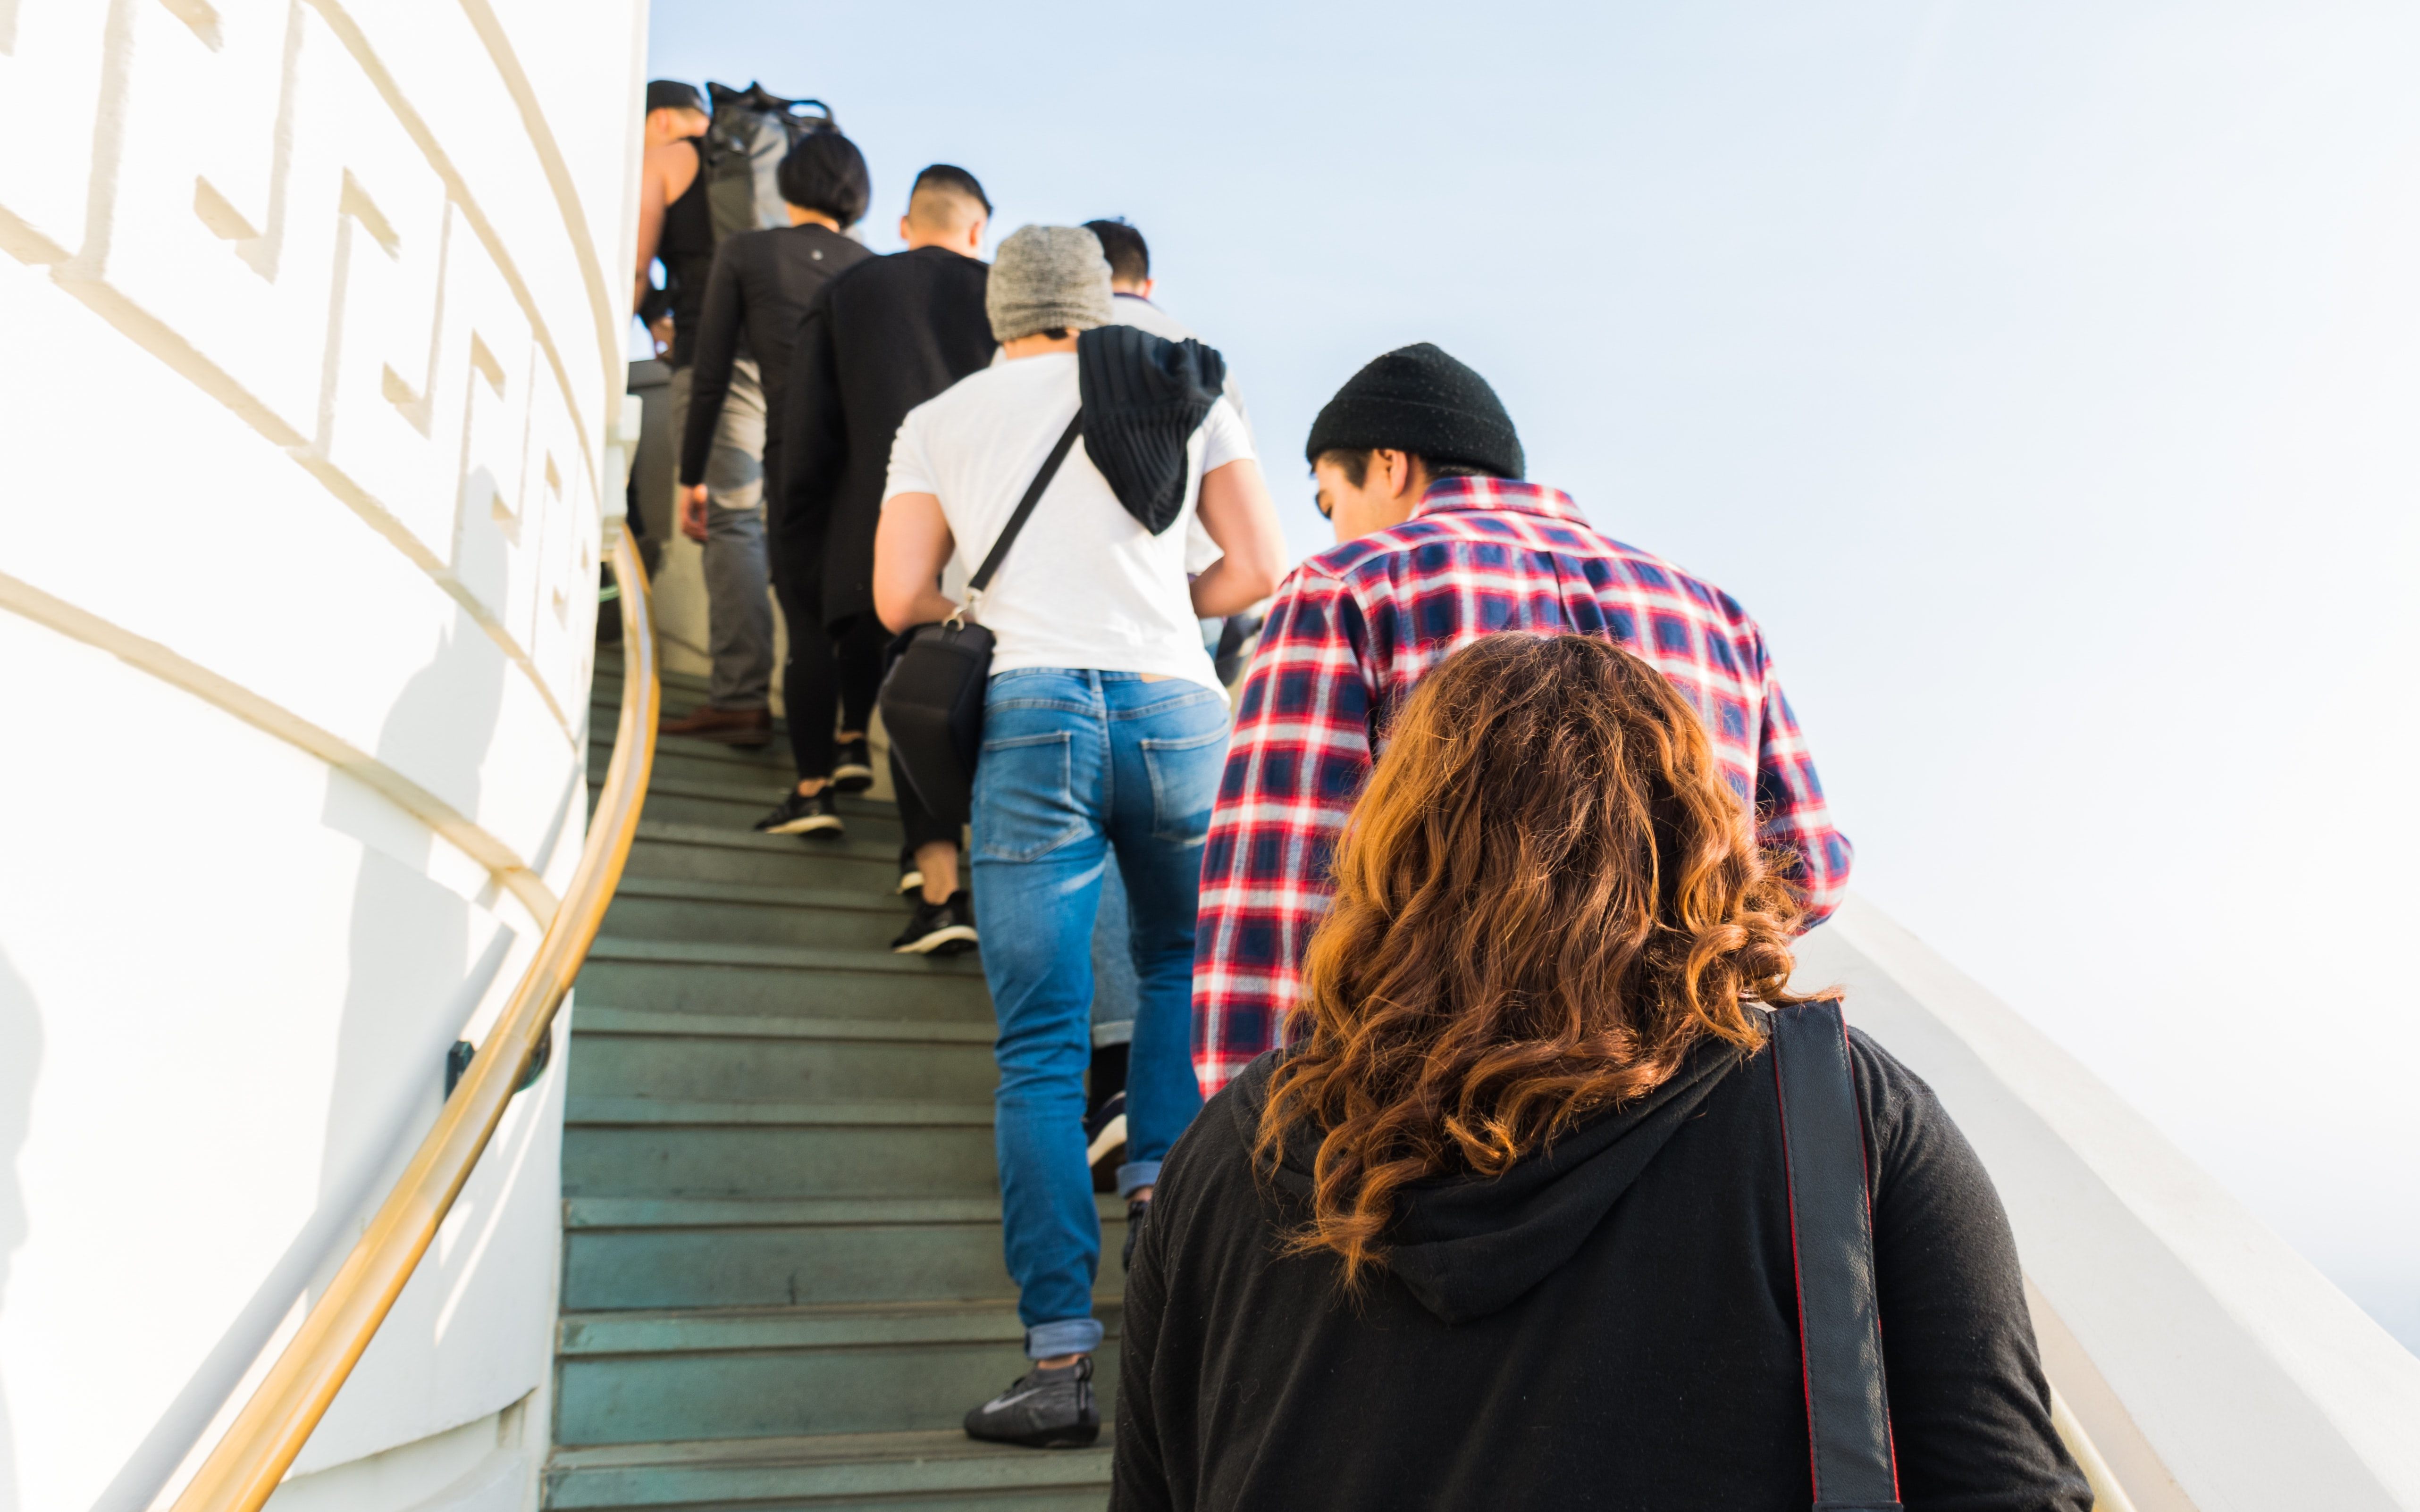
\includegraphics[keepaspectratio, width=12cm, height=9cm]{imagens/06/06 - waiting queue.jpg}
\caption{Fila de espera   \\
Autor: Levi Jones, de: unsplash.com \\}
\label{fig:Fila de espera}
\end{figure}



Para solucionar esse gargalo, poderíamos pensar em alocar, para cada
tarefa, uma parcela de tempo, digamos 10 minutos, de forma que, após
esgotado esse tempo, você terá que alterar a tarefa a ser executada,
independente se a mesma foi concluída ou não, passando para a próxima
não interdependente (\emph{non-blocking}). Assim, o leitor iniciaria o
processo chamando o primeiro da fila. Após 10 minutos, caso o
atendimento não seja concluído (por exemplo, o cliente ainda não tenha
escolhido o produto que quer), essa tarefa atualmente em trabalho será
deixada de lado (entrando no estado de espera), e a próxima tarefa não
interdependente (que no caso seria chamar o próximo da fila) deverá ser
executada. A vantagem dessa abordagem é que o tempo dentro da fila de
espera deve cair substancialmente, pois aproveita-se o tempo (no qual,
anteriormente, você ficava ocioso) de escolha (de um produto) de um
cliente, atendendo o próximo da fila.
Essa abordagem também trás desvantagens. Primeiro, você terá que
administrar (e muito bem) a prioridade e a alternância entre tarefas,
aumentando assim a complexidade do ciclo. Os clientes que fazem escolhas
rápidas podem não ficar contentes em ter que esperar que outras tarefas
relacionadas com outros compradores sejam concluídas (ou que entrem no
estado de espera) previamente, ocorrência que diminui o tempo de
resposta (responsividade) do processo. Igualmente, um número suficiente
de compradores pode tornar a responsividade tão baixa que os clientes,
simplesmente, desistirão do atendimento, derrubando a qualidade
percebida e, a loja, deixando de realizar a venda. A imposição de
padrões de qualidade (como um tempo máximo de espera por cliente), pode
resolver o problema anterior, mas criar outros, como a loja negar a
servir mais que uma quantidade específica de pessoas por período de
tempo (analogamente, ataque DDoS).
Pode-se pensar também em abrir uma segunda (ou terceira, quarta, etc)
loja ao lado, com um colaborador cada, de forma que mais clientes possam
ser atendidos. Porém, novos recursos (como caixa, material lampadas,
etc) terão que ser adquiridos, demandando tempo e dinheiro para tal.
Então, a solução mais simples (e com diversas vantagens) é a contratação
de empregados para que múltiplas tarefas possam ser desempenhadas em
paralelo, como mostrado na Figura \ref{fig:Três trabalhos em paralelo}.

\begin{figure}[h!]
\centering
\includegraphics[keepaspectratio, width=12cm, height=9cm]{imagens/06/06 - dois trabalhos em simultâneo.jpg}
\caption{Três trabalhos em paralelo   \\
Autor: Charlie Firth de: Unsplash \\}
\label{fig:Três trabalhos em paralelo}
\end{figure}


A história acima é uma analogia ao que ocorre nos sistemas
computacionais modernos, de forma que:

• O processo (em um sistema operacional) é equivalente à loja. •
Funcionários são como \emph{threads}. • Os recursos da loja (caixa,
material lampadas, etc) são como os recursos computacionais (como a
memória). • O ciclo de venda é o serviço oferecido pelo sistema
computacional. • E assim em diante.

Essa comparação é interessante pois a mesma pergunta vem à tona: devemos
criar um novo processo (abrir uma nova loja) ou, simplesmente, criar
novas \emph{threads} (contratar colaboradores) ?

O capítulo atual foi dividido em:

• Identificar os componentes de uma \emph{thread}. • Benefícios e
desafios. • \emph{Threads} e o Linux. (descrever como as \emph{threads}
são representadas no Linux e projetar uma aplicação). • Complementar

\hypertarget{identificar-os-componentes-de-uma-thread.}{%
\section{\texorpdfstring{Identificar os componentes de uma
\emph{thread}.}{Identificar os componentes de uma thread.}}\label{identificar-os-componentes-de-uma-thread.}}

A \emph{Thread} (unidade de processamento do processo) é composto pela
\emph{thread id} (seu identificador único), PC (\emph{program counter}),
valores dos registradores, memória \emph{stack}. Ela compartilha, com
outras \emph{theads} do mesmo processo, recursos como as sessões de
memória \emph{text}, \emph{data} e os arquivos abertos, como mostrado na
Figura \ref{fig:Processos com uma ou múltiplas threads}.


\begin{figure}[h!]
\centering
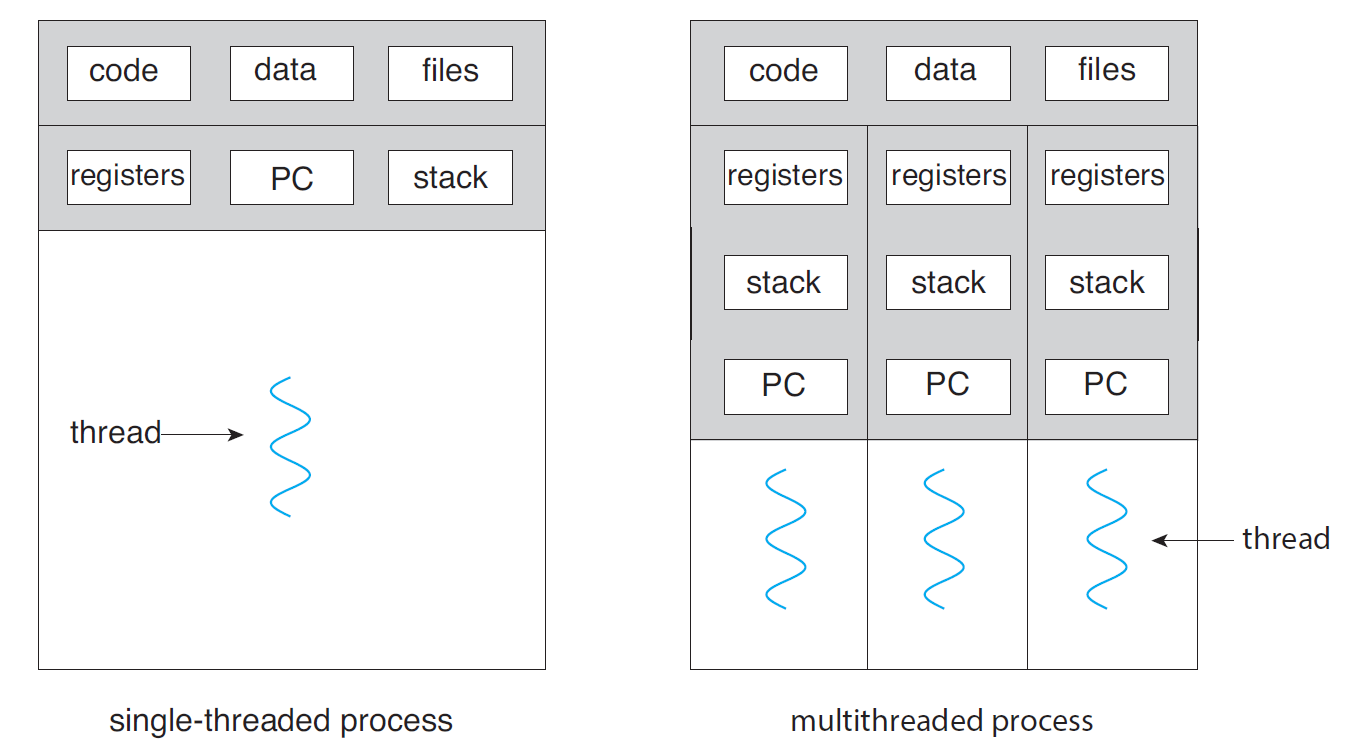
\includegraphics[keepaspectratio, width=16cm, height=15cm]{imagens/06/06 - single threaded x multi threaded.png}
\caption{Processos com uma ou múltiplas threads   \\
Imagem retirada de: Silberschatz, A. Operating System Concepts, 10th,
página 160. \\}
\label{fig:Processos com uma ou múltiplas threads}
\end{figure}



\hypertarget{benefuxedcios-e-desafios.}{%
\section{Benefícios e Desafios.}\label{benefuxedcios-e-desafios.}}

\hypertarget{benefuxedcios.}{%
\subsubsection{Benefícios.}\label{benefuxedcios.}}

Em sistemas com múltiplos núcleos de processamento, as \emph{threads}
podem trazer várias vantagens, como:

1.Responsividade: Um programa continua rodando mesmo quando uma parte
sua é bloqueada, trava ou demora para concluir. 2.Compartilhamento de
Recursos: As Threads compartilham o mesmo código e dados por padrão.
3.Economia: é mais econômico criar uma Thread do que um processo. É mais
rápido trocar o contexto da CPU (CPU context-switch) entre Threads do
que entre processos, desde que estejam em userspace. 4.Escalabilidade:
Threads podem usufruir do paralelismo, rodando em múltiplas CPU's em
simultâneo de forma assíncrona.

\hypertarget{desafios.}{%
\subsubsection{Desafios.}\label{desafios.}}

\begin{enumerate}
\def\labelenumi{\arabic{enumi}.}
\tightlist
\item
  Identificar tarefas: examinar a aplicação e separá-la em diferentes
  tarefas que possam ser executadas em paralelo.
\item
  Balancear: a carga de trabalho deve ser distribuída entre as tarefas
  (idealmente, as tarefas teriam a mesma carga).
\item
  Divisão de dados: os dados devem sem divididos para rodar em núcleos
  de processamento separados (para evirar a \emph{race condition}).
\item
  Dependência de dados: os programadores devem garantir que as tarefas
  estejam sincronizadas quando uma \emph{thread} depende dos dados de
  outra.
\item
  Teste: é mais difícil testar e replicar casos de erro em sistemas com
  múltiplas \emph{threads} em comparação com as de \emph{thread} única.
\end{enumerate}

\hypertarget{modelos-de-multithread}{%
\section{Modelos de multithread}\label{modelos-de-multithread}}

Há dois tipos diferentes de \emph{threads}, aquelas que estão no nível
de usuário, sendo gerenciadas sem ajuda do \emph{kernel}, e aquelas que
estão no nível do \emph{kernel}, que são gerenciadas diretamente pelo
sistema operacional. Assim, os modelos de \emph{multithread} definem o
relacionamento desses dois tipos de \emph{threads}.


\begin{enumerate}
\def\labelenumi{\arabic{enumi}.}

\item
  \emph{Many-to-one} (Figura \ref{fig:Modelo Many-to-One}): nesse modelo, várias \emph{threads} de nível do
  usuário são mapeadas para uma única \emph{thread} de \emph{kernel}.
\item
  \emph{One-to-one} (Figura \ref{fig:Modelo One-to-One}): cada \emph{thread} de usuário tem, mapeada, uma
  \emph{thread} de \emph{kernel}.
\item
  \emph{Many-to-many} (Figura \ref{fig:Modelo Many-to-Many}): várias \emph{threads} de usuário são
  multiplexadas entre as diferentes \emph{threads} de kernel.
\item
  \emph{Two-level} (Figura \ref{fig:Modelo two-level}): esse modelo une o \emph{one-to-one} com o
  \emph{many-to-many}.
\end{enumerate}



\begin{figure}[h!]
\centering
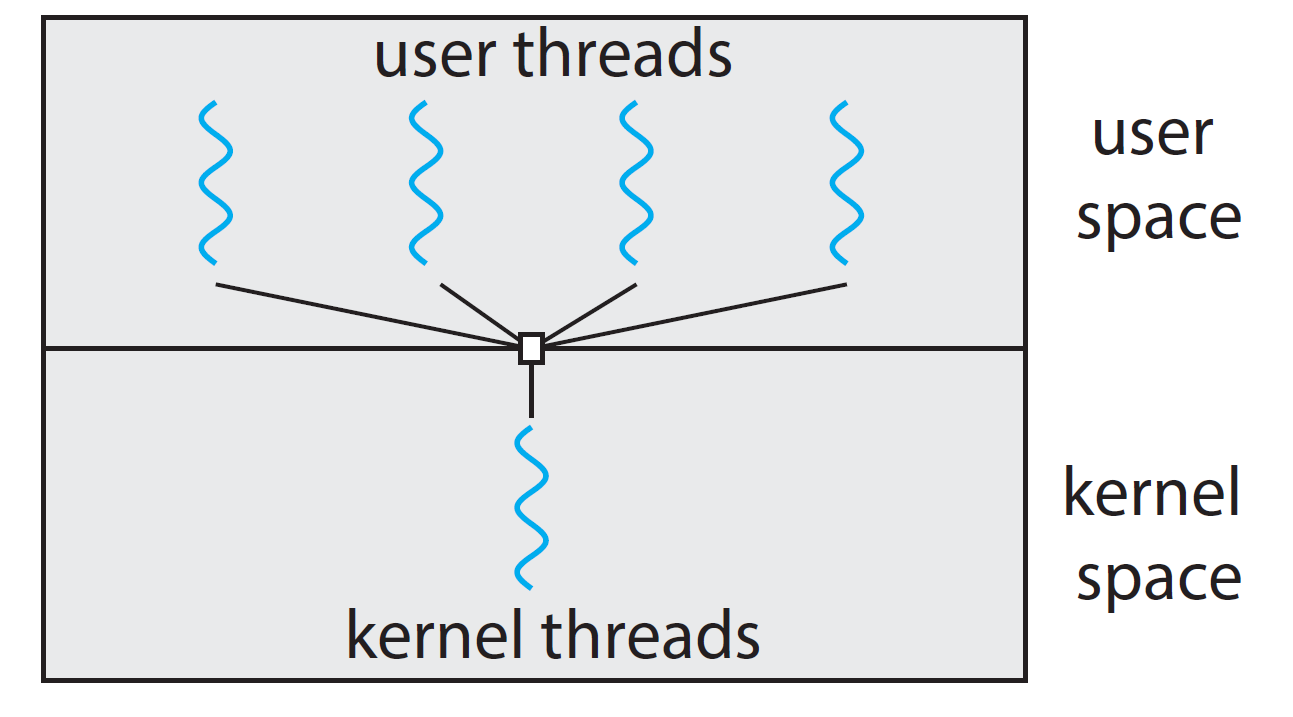
\includegraphics[keepaspectratio, width=12cm, height=9cm]{imagens/06/06 - many-to-one.png}
\caption{Modelo Many-to-One   \\
Imagem retirada de: Silberschatz, A. Operating System Concepts, 10th,
página 166. \\}
\label{fig:Modelo Many-to-One}
\end{figure}

\begin{figure}[h!]
\centering
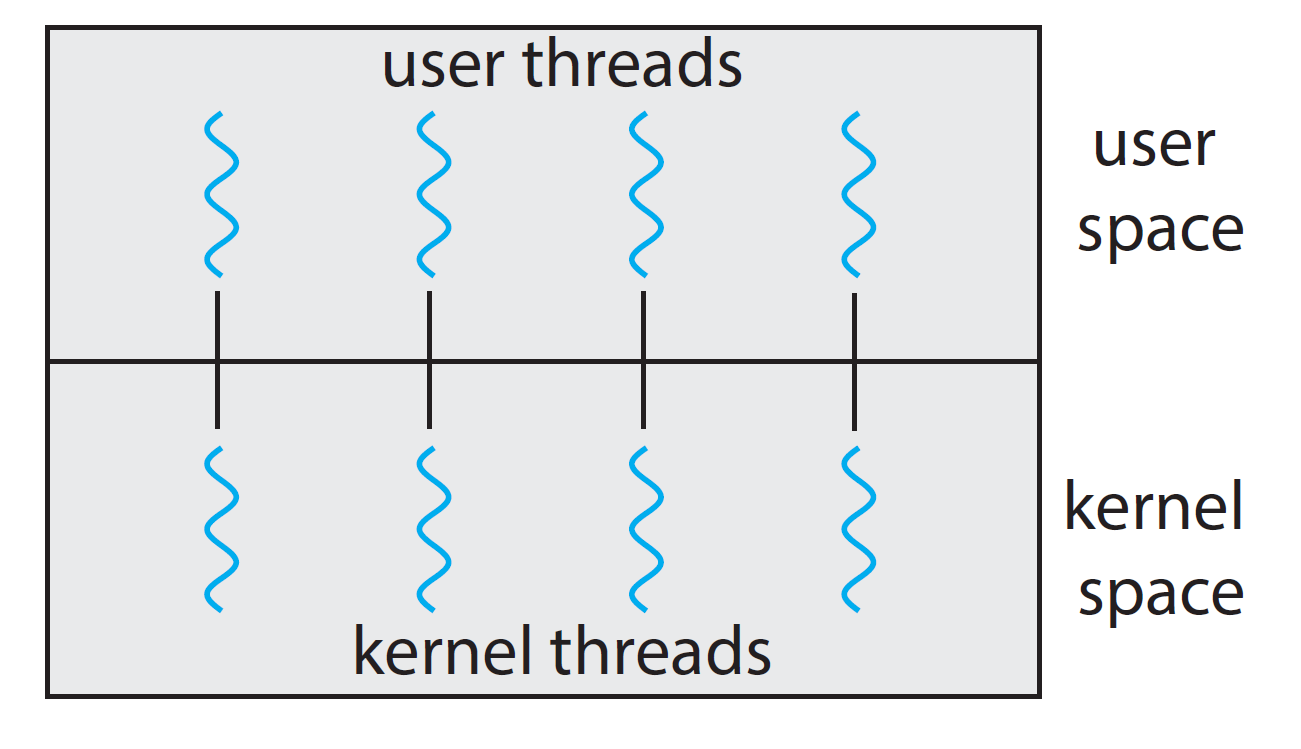
\includegraphics[keepaspectratio, width=12cm, height=9cm]{imagens/06/06 - one-to-one.png}
\caption{Modelo One-to-One   \\
Imagem retirada de: Silberschatz, A. Operating System Concepts, 10th,
página 167. \\}
\label{fig:Modelo One-to-One}
\end{figure}

\begin{figure}[h!]
\centering
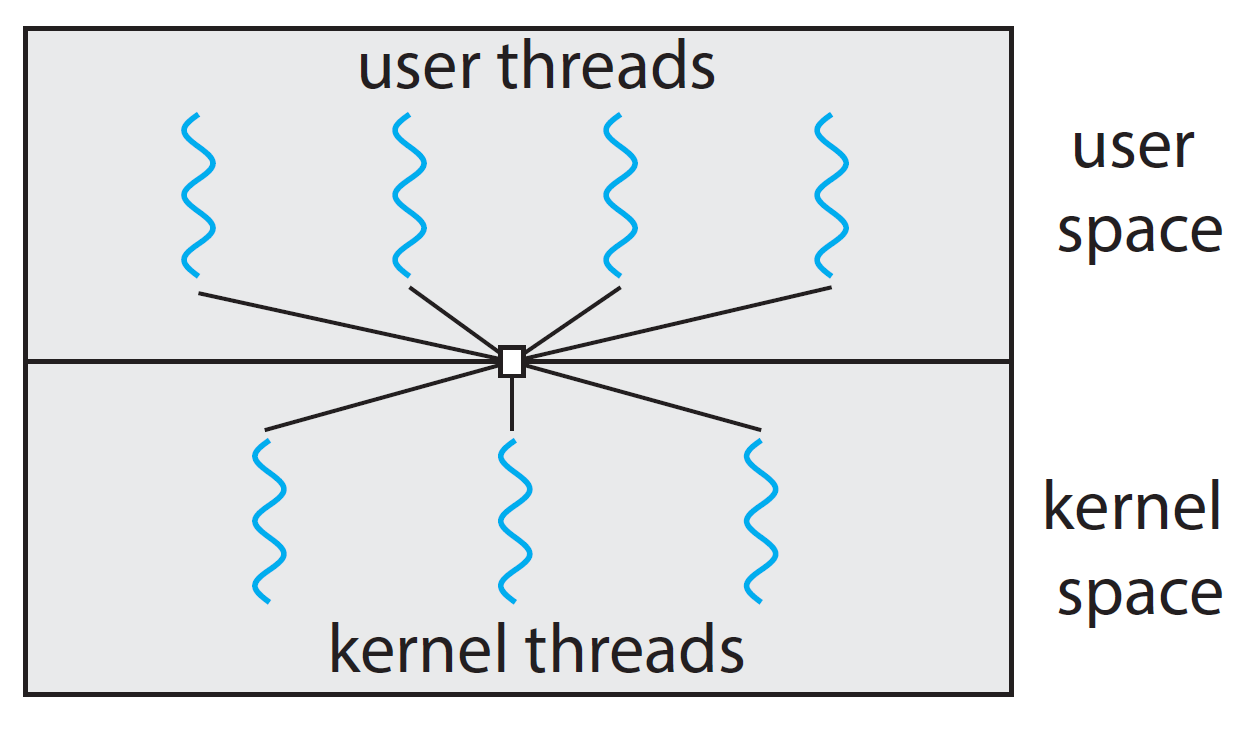
\includegraphics[keepaspectratio, width=12cm, height=9cm]{imagens/06/06 - many-to-many.png}
\caption{Modelo Many-to-Many  \\
Imagem retirada de: Silberschatz, A. Operating System Concepts, 10th,
página 167. \\}
\label{fig:Modelo Many-to-Many}
\end{figure}


\begin{figure}[h!]
\centering
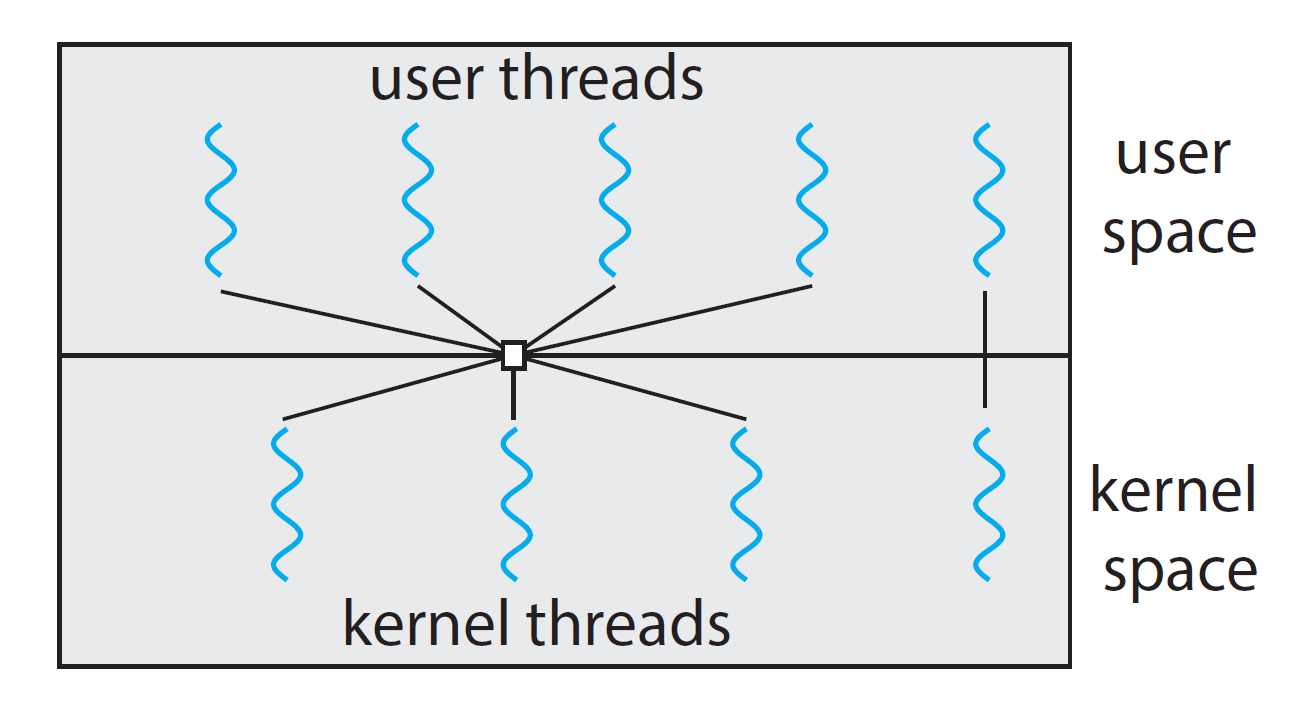
\includegraphics[keepaspectratio, width=12cm, height=9cm]{imagens/06/06 - two-level.png}
\caption{Modelo two-level  \\
Imagem retirada de: Silberschatz, A. Operating System Concepts, 10th,
página 168. \\}
\label{fig:Modelo two-level}
\end{figure}


\hypertarget{threads-e-o-linux}{%
\section{Threads e o Linux}\label{threads-e-o-linux}}

\hypertarget{biblioteca-pthread}{%
\subsection{\texorpdfstring{Biblioteca
\texttt{pthread}}{Biblioteca pthread}}\label{biblioteca-pthread}}

O Linux utiliza a biblioteca POSIX \emph{threads}, nomeada, em
\texttt{C}, de \texttt{pthread}.

O exemplo a seguir foi retirado de: Silberschatz, A. Operating System
Concepts, 10th, página 170.*


\begin{minted}[mathescape, linenos]{c}

    #include <pthread.h>
    #include <stdio.h>
    #include <stdlib.h>
    
    int sum; /* this data is shared by the thread(s) */
    void *runner(void *param); /* threads call this function */
    
    int main(int argc, char *argv[])
    {
        pthread_t tid; /* the thread identifier */
        pthread_attr_t attr; /* set of thread attributes */
        /* set the default attributes of the thread */
        pthread_attr_init(&attr);
        /* create the thread */
        pthread_create(&tid, &attr, runner, argv[1]);
        /* wait for the thread to exit */
        pthread_join(tid,NULL);
        printf("sum = %d∖n",sum);
    }
    
    /* The thread will execute in this function */
    void *runner(void *param)
    {
        int i, upper = atoi(param);
        sum = 0;
        for (i = 1; i <= upper; i++)
        sum += i;
        pthread exit(0);
    }
    
\end{minted}


\hypertarget{semuxe1foros}{%
\subsection{Semáforos}\label{semuxe1foros}}

A execução em paralelo de várias \emph{threads} (de dados
compartilhados) pode gerar uma \emph{race condition} (conceito debatido
em capítulos anteriores) por poder alterar, com dados desatualizados, o
mesmo valor. Considere:

\begin{minted}[mathescape, linenos]{c}

    int a = 5;
    a = a - 1;
    
\end{minted}



A \emph{thread} ``A'' e ``B'', executando em paralelo, podem gerar o
resultado final de 4, e não de 3, como esperado, Pois:

\begin{enumerate}
\def\labelenumi{\arabic{enumi}.}
\tightlist
\item
  \emph{Thread} ``A'' coleta o valor de \texttt{a} (5).
\item
  \emph{Thread} ``B'' coleta o valor de \texttt{a} (5).
\item
  \emph{Thread} ``B'' calcula \texttt{a\ -\ 1} (4).
\item
  \emph{Thread} ``A'' calcula \texttt{a\ -\ 1} (4).
\item
  \emph{Thread} ``A'' ajusta o valor de \texttt{a} (4).
\item
  \emph{Thread} ``B'' ajusta o valor de \texttt{a} (4).
\end{enumerate}

Esse caso fica visível no exemplo a seguir:

Exemplo retirada de: Griffiths, David; Griffiths, Dawn; Head First C,
página 510.

\begin{minted}[mathescape, linenos]{c}

    #include <stdio.h>
    #include <stdlib.h>
    #include <string.h>
    #include <unistd.h>
    #include <errno.h>
    #include <pthread.h>
    
    int beers = 2000000;
    void* drink_lots(void *a)
    {
    int i;
    for (i = 0; i < 100000; i++) {
    beers = beers - 1;
    }
    return NULL;
    }
    int main()
    {
    pthread_t threads[20];
    int t;
    printf("%i bottles of beer on the wall\n%i bottles of beer\n", beers, beers);
    for (t = 0; t < 20; t++) {
    ( , NULL, , NULL);
    }
    void* result;
    for (t = 0; t < 20; t++) {
    pthread_create(threads[t], &result);
    }
    printf("There are now %i bottles of beer on the wall\n", beers);
    return 0;
    }
    pthread_join
    &threads[t]
    drink_lots
    
\end{minted}


no qual, o trecho abaixo (região crítica) necessita ser protegido pelo
acesso múltiplo, como explicado anteriormente.

\begin{minted}[mathescape, linenos]{c}

    for (i = 0; i < 100000; i++) {
        beers = beers - 1;
    }
    
\end{minted}



Sem essa proteção, os resultados serão:

Resultados retirados de: Griffiths, David; Griffiths, Dawn; Head First
C, página 511.

\begin{lstlisting}[language=bash]
    > ./beer 
    2000000 bottles of beer on the wall 
    2000000 bottles of beer 
    There are now 0 bottles of beer on the wall 
    > ./beer 
    2000000 bottles of beer on the wall 
    2000000 bottles of beer 
    There are now 883988 bottles of beer on the wall 
    > ./beer 2000000 bottles of beer on the wall 
    2000000 bottles of beer 
    There are now 945170 bottles of beer on the wall ```
\end{lstlisting}



Perceba que, sem proteção, os resultados não são consistentes.

Para que essas duas \emph{threads} trabalhem de forma síncrona, é
necessário que haja um semáforo (mesmo conceito de controle de tráfego
de carros), para o controle de acesso, como mostrado na Figura \ref{fig:Semáforo para controle de acesso.}. Os
semáforos que previnem que as \emph{threads} não se choquem são chamadas
de \texttt{mutex} (\emph{mutually exclusive}, só permite uma única
\emph{thread} na região crítica) e também de \texttt{locks}.


\begin{figure}[h!]
\centering
\includegraphics[keepaspectratio, width=12cm, height=9cm]{imagens/06/06 - semáforo.png}
\caption{Semáforo para controle de acesso.  \\
Imagem retirada de: Griffiths, David; Griffiths, Dawn; Head First C,
página 513. \\}
\label{fig:Semáforo para controle de acesso.}
\end{figure}



Existem, então, duas soluções para o trecho de código anterior, cada
qual gerará resultados de saída, desempenho e sincronicidade diferentes.

Solução A.


\begin{minted}[mathescape, linenos]{c}

    pthread_mutex_t beers_lock = PTHREAD_MUTEX_INITIALIZER;
    
    void* drink_lots(void *a)
    {
        int i;
        pthread_mutex_lock(&beers_lock);
        
        for (i = 0; i < 100000; i++) {
            beers = beers - 1;
        }
        
        pthread_mutex_unlock(&beers_lock);
        printf("beers = %i\n", beers);
        return NULL;
    }
    
\end{minted}





Solução B.

\begin{minted}[mathescape, linenos]{c}

    pthread_mutex_t beers_lock = PTHREAD_MUTEX_INITIALIZER;
    
    void* drink_lots(void *a)
    {
        int i;
        
        for (i = 0; i < 100000; i++) {
            pthread_mutex_lock(&beers_lock);
            beers = beers - 1;
            pthread_mutex_unlock(&beers_lock);
        }
        
        printf("beers = %i\n", beers);
        return NULL;
    }
    
\end{minted}



Resultados retirados de: Griffiths, David; Griffiths, Dawn; Head First
C, página 517.

Resultado Versão A.

\begin{lstlisting}[language=bash]
    > ./beer
    2000000 bottles of beer on the wall
    2000000 bottles of beer
    beers = 1900000
    beers = 1800000
    beers = 1700000
    beers = 1600000
    beers = 1500000
    beers = 1400000
    beers = 1300000
    beers = 1200000
    beers = 1100000
    beers = 1000000
    beers = 900000
    beers = 800000
    beers = 700000
    beers = 600000
    beers = 500000
    beers = 400000
    beers = 300000
    beers = 200000
    beers = 100000
    beers = 0
    There are now 0 bottles of beer on the wall
    >
\end{lstlisting}



Resultado Versão B.

\begin{lstlisting}[language=bash]
    > ./beer_fixed_strategy_2
    2000000 bottles of beer on the wall
    2000000 bottles of beer
    beers = 63082
    beers = 123
    beers = 104
    beers = 102
    beers = 96
    beers = 75
    beers = 67
    beers = 66
    beers = 65
    beers = 62
    beers = 58
    beers = 56
    beers = 51
    beers = 41
    beers = 36
    beers = 30
    beers = 28
    beers = 15
    beers = 14
    beers = 0
    There are now 0 bottles of beer on the wall
>

\end{lstlisting}



\hypertarget{complementar-2}{%
\section{Complementar}\label{complementar-2}}

\hypertarget{tuxe9cnicas-de-paralelismo.}{%
\subsection{Técnicas de
paralelismo.}\label{tuxe9cnicas-de-paralelismo.}}

Fundamentalmente, existem dois tipos diferentes de paralelismo, o
paralelismo de tarefas (\emph{task parallelism}), que consiste em
dividir múltiplas tarefas compartilhando os dados necessários, e o
paralelismo de dados (\emph{data parallelism}), o qual há uma
distribuição dos dados sobre as tarefas.


\begin{figure}[H]
\centering
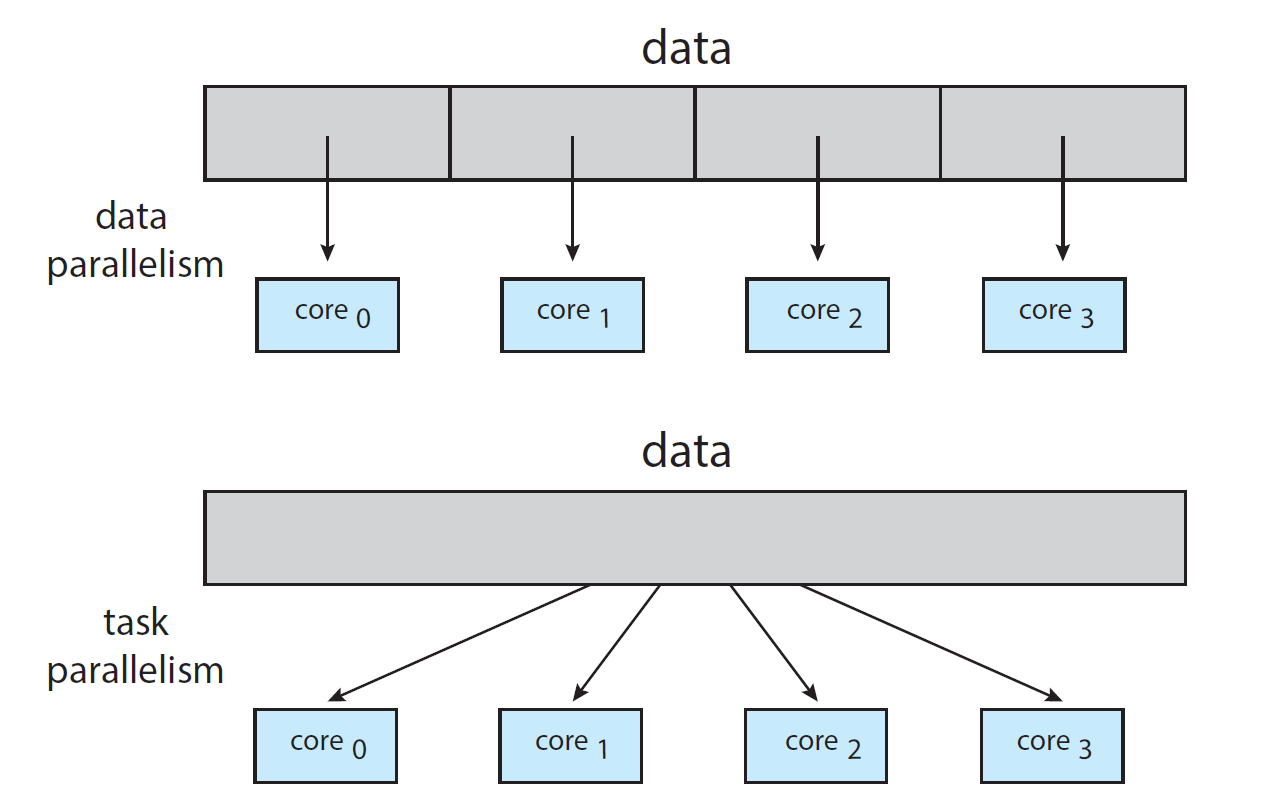
\includegraphics[keepaspectratio, width=12cm, height=9cm]{imagens/06/06 - data and task parallelism.png}
\caption{Processos com uma ou múltiplas threads  \\
Silberschatz, A. Operating System Concepts, 10th, página 170. \\
}
\label{fig:Processos com uma ou múltiplas threads}
\end{figure}


%\hypertarget{aula-7---redes.}{%
%\chapter{Aula: 7}\label{aula-7}}



\hypertarget{introduuxe7uxe3o-uxe0-redes-de-computadores}{%
\chapter{Introdução à redes de
computadores}\label{introduuxe7uxe3o-uxe0-redes-de-computadores}}

A Internet é uma rede mundial de computadores que interconecta, por meio
de \emph{communication links}, bilhões de dispositivos \emph{hosts}
(anfitriões), também referidos como \emph{end systems} (sistemas finais)
por estarem na borda de internet, como os clientes (computadores
pessoais) e servidores. Seu funcionamento é análogo ao modal de
transporte rodoviário, pois assim como um produto, que ao sair de uma
manufatura, deve ser empacotado, carregado no caminhão, transportado
através das rodovias, descarregado no destino, e desempacotado, para em
fim estar disponível para uso, os dados também passam pelo mesmo
processo, pois ao sair de um \emph{host}, devem ser empacotados,
carregados no protocolo de transmissão (como \emph{Transmission Control
Protocol} e \emph{Internet Protocol}, que definem o formato, utilizando
o \emph{struct} na linguagem \texttt{c}, e a ordem das mensagens),
transportados por um meio físico (como cabos ou espectro
eletromagnético), descarregados do protocolo no destino, e
desempacotados, para finalmente serem usados por alguma aplicação.

É importante citar que os protocolos de Internet são desenvolvidos pela
\emph{Internet Engineering Task Force} (IETF) e os seus documentos são
chamados de \emph{requests for comments} (RFCs).

Essa rede pode também ser definida como uma plataforma que oferece
serviços de comunicação entre aplicações, tornando-se, dessa forma,
análogo à um sistema de correios que oferece serviços aos seus clientes
como entrega normal ou expressa.

O acesso à internet é fornecido por ISPs (\emph{Internet Service
Providers), que transmitem os dados de forma guiada (}guided
media\emph{), através, por exemplo, de cabos de cobre de par trançado,
redes de telefone (com o DSL, }Digital Subscriber Line\emph{), cabos de
televisão ou fibra optica (com o conceito }fiber to the home\emph{, ou
FTTH), ou de forma não guiada (}unguided media*), no qual ondas
eletromagnéticas propagam-se pela atmosfera e espaço, com o uso das
torres de rádio e dos satélites (como os geoestacionários, que
introduzem um atraso de 280 milissegundos na comunicação, e os de baixa
órbita).



%\hypertarget{aula-8}{%
%\chapter{Aula: 8}\label{aula-8}}




\hypertarget{internet-a-rede-das-redes}{%
\chapter{Internet: a rede das
redes}\label{internet-a-rede-das-redes}}

Atualmente, é cada vez mais comum encontramos dispositivos, como
impressoras e celulares, que são capazes de interconectar-se e trabalhar
em conjunto, formando uma rede de comunicação. Nas residências e
empresas, essa rede de comunicação é chamada de LAN (\emph{Local Area
Network} ou rede de acesso local), pois tem um alcance limitado.

Essas redes podem ter seu alcance ampliado, a partir de uma
interconexão, para uma cidade inteira, algo que forma a MAN
(\emph{Metropolitan Area Network}). Por fim, é possível amplificar o
alcance das MAN's, vinculando-as para, assim, gerar a WAN (\emph{Wide
Area Network}), uma rede que engloba regiões e países. A internet é
advinda da interconexão de múltiplas WAN's.

O usuário final tem acesso à internet através das ISP's (\emph{Internet
Service Provider}) municipais. Essas tem a comunicação estabelecida por
ISP's regionais e nacionais (que, geralmente, não fornecem seus serviços
aos clientes finais), ou \emph{tier 1 ISP's}. Por fim, essas últimas
interconectam-se diretamente ou através de IXP's (\emph{Internet
Exchange Point}) e CPN's (\emph{content-provider networks} ou redes de
provedores de conteúdo), como o Google, que vincula-se externamente, com
os IXP's e ISP's, e internamente, com uma rede privada inacessível ao
público. A Figura \ref{fig:Rede de redes } mostra, de uma forma gráfica, a rede de redes.

\begin{figure}[h!]
\centering
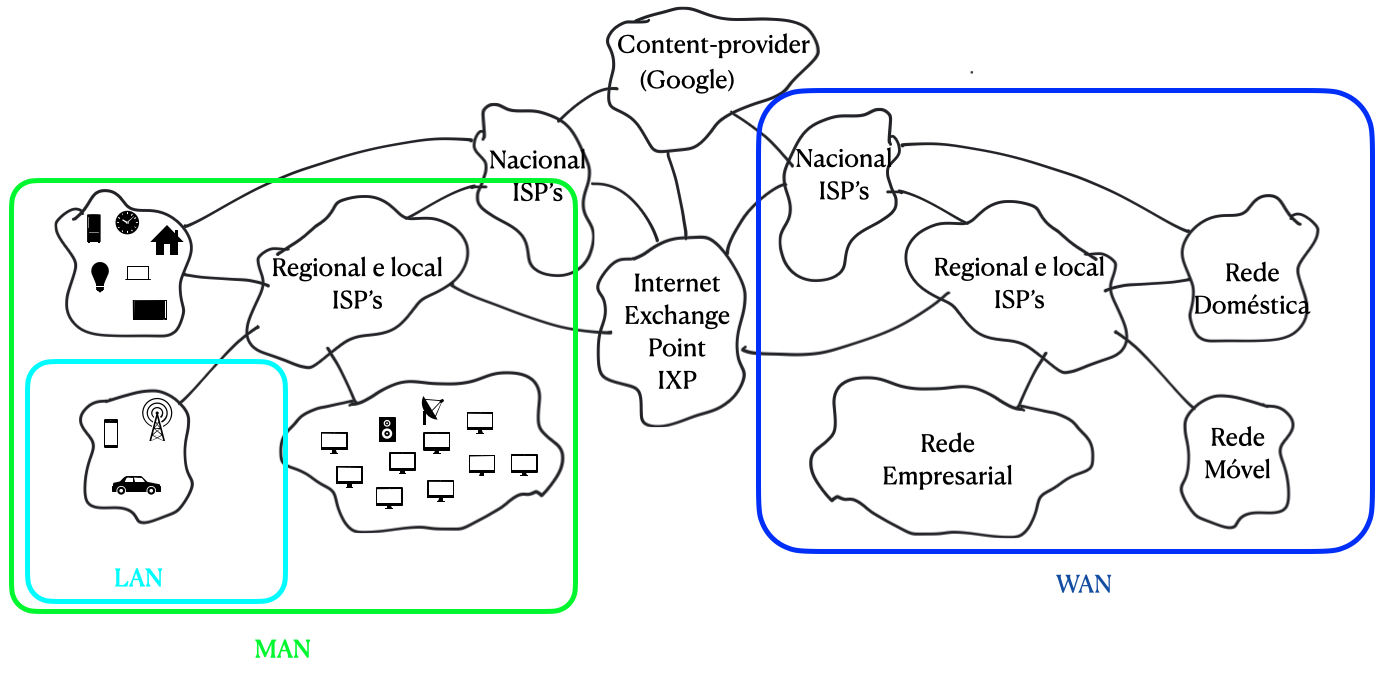
\includegraphics[keepaspectratio, width=14cm, height=13cm]{imagens/08/08 - redes.png}
\caption{Rede de redes  \\}
\label{fig:Rede de redes }
\end{figure}



\hypertarget{dispositivos}{%
\section{Dispositivos}\label{dispositivos}}

De forma simplificada, a rede LAN tem a mesma estrutura das demais,
contendo o modem, responsável por conectar diferentes redes, o roteador,
o qual gerencia a rota de tráfego dos dados, e o switch, que
interconecta diversos dispositivos na mesma rede. É importante dizer que
essas funcionalidades podem estar contidas em um ou mais dispositivos.

\hypertarget{roteador}{%
\subsection{Roteador}\label{roteador}}

Os roteadores são computadores de propósito específico, sendo otimizados
para operar as camadas de rede, enlace e física (a primeira em
destaque). Executam programas para configurações, com sua página HTML
enviando comandos ao shell do Linux (sistema operacional normalmente
encontrado nesses dispositivos). São responsáveis por mover os pacotes
de entrada para a sua saída apropriada. Para tal, é utilizado uma tabela
de encaminhamento, no qual a determinação do \emph{link} que a mensagem
deve ser transmitida é feita a partir do \emph{IP address} (endereço do
computador no procolo de internet), que está localizado no \emph{header}
adicionado pela camada \emph{network}. Nos sistemas mais antigos, o
algoritmo de roteamento estava contido no roteador, porém, com o aumento
da complexidade das redes, esse algoritmo foi desacoplado do roteador,
passando para um servidor que atualiza a tabela de encaminhamento (que
pode ser entendida como uma configuração da rede), sistema chamado de
\emph{software define networks} (trazendo vantagens como a velocidade de
operação do roteador). Esse sistema de configuração de rede ocorre no
\emph{core} da rede, e não nas bordas, pois, por exemplo, em redes
domésticas (que se encontram na borda), isso não é necessário pelo fato
de somente haver uma única entrada e saída (assim não precisa de
configuração).

\hypertarget{Transmissão}{%
\section{Transmissão}\label{transmissuxe3o}}

A transmissão dos dados entre os dispositivos é feito através de 5
camadas, iniciando-se a partir da camada de aplicação, que ocorre no
\emph{user space}, local de origem da mensagem (enviado em pedaços de
dados intitulado de \emph{packets}, ou pacotes), passando por transporte,
rede (com ambas estando no \emph{kernel space}), enlace (com uma parte
do software no \emph{kernel space} e parte em \emph{hardware}) e física
(encontrada somente em \emph{hardware}), no qual cada uma encapsula os
dados das camadas anteriores e adiciona o seu \emph{header}, tendo como
saída, respectivamente, os chamados \emph{segment}, \emph{datagram},
\emph{frame} e a série de sinais físicos que representam os \emph{bits}.
As duas últimas camadas, enlace e física, são implementadas pela NIC
(\emph{Network Interface Card}, ou placa de rede).

O receptor desses dados fará o processo inverso, extraindo o
\emph{header} de sua respectiva camada de forma a desencapsular o
pacote, até que a mensagem seja entregue para a aplicação receptora,
como mostrado na Figura \ref{fig:Emissor e receptor dos dados }.

\begin{figure}[h!]
\centering
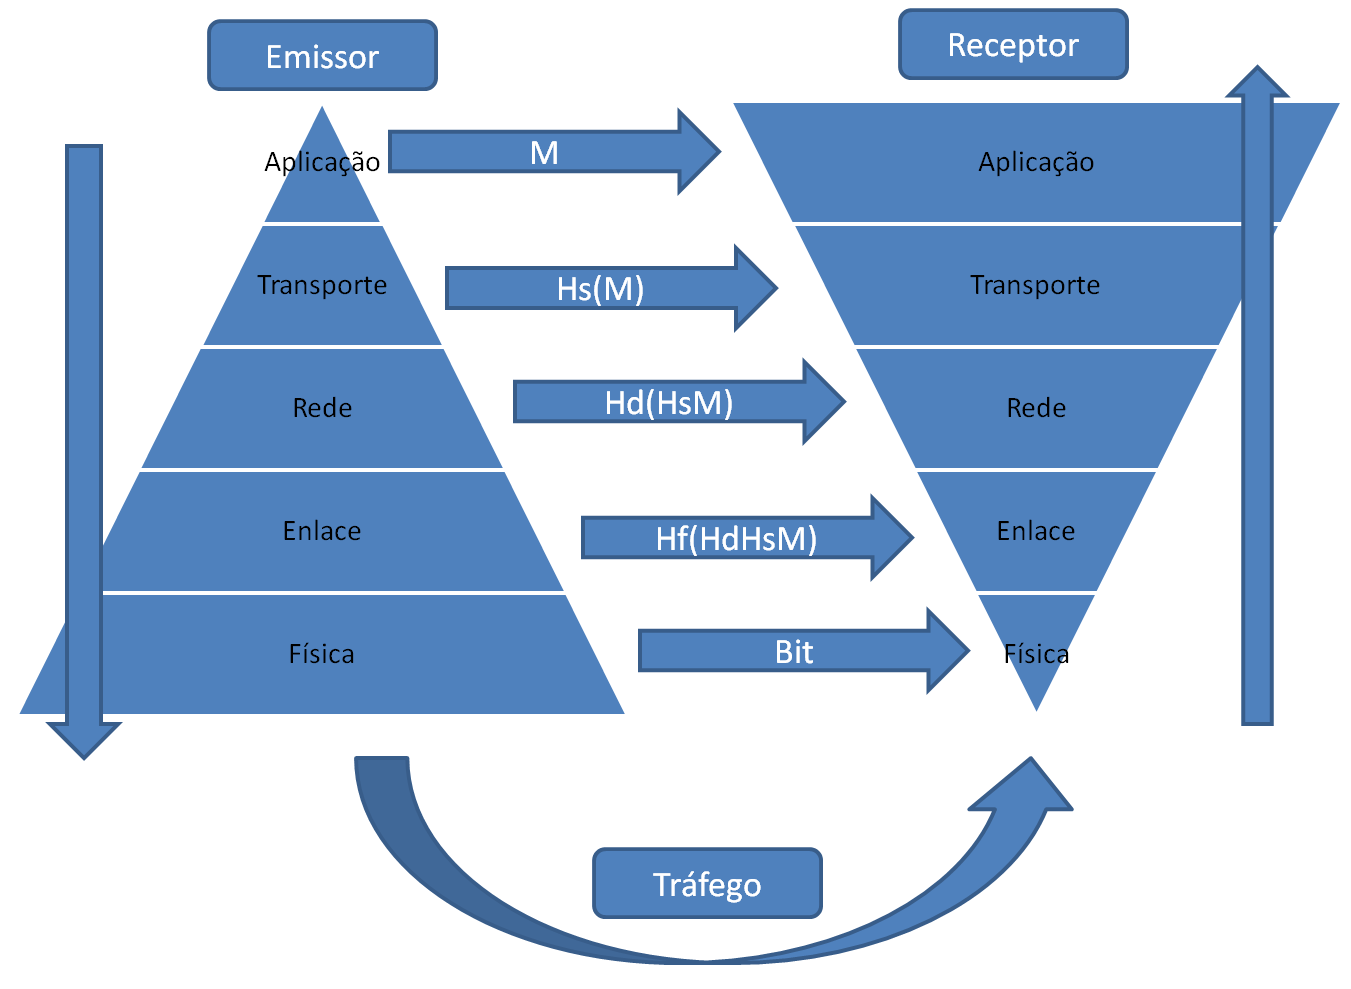
\includegraphics[keepaspectratio, width=12cm, height=9cm]{imagens/08/08 - Emissor e receptor dos dados.png}
\caption{Emissor e receptor dos dados  \\}
\label{fig:Emissor e receptor dos dados }
\end{figure}



É interessante perceber que essa arquitetura de protocolos empilhados
transforma cada camada em uma provedora de serviços à camada superior,
algo que torna o sistema modular, fácil de ser atualizado e fácil de ser
debatido e explicado. Porém, esses sistema de camadas pode conter
duplicações de funcionalidade e de informação.

Normalmente a transmissão não ocorre de um modo direto entre o emissor e
o receptor, e sim aliado também aos dispositivos já mencionados
anteriormente, como o \emph{switch}. Esses aparelhos utilizam de algumas
camadas para a sua operação, como a de rede, enlaço e física para o
roteador, procedendo com o desencapsulamento dos dados recebidas e o
encapsulamento com o seu protocolo, para assim repassá-las adiante.

\hypertarget{packet-switching-store-and-forward}{%
\subsection{Packet-switching: store-and-forward}\label{packet-switching-store-and-forward}}

O repasse dos dados é feita utilizando a técnica \emph{store and
fowarding}, no qual cada pacote ``pula'' de um dispositivo para o outro,
sendo primeiro armazenado (store) e em seguida repassado (fowarding).
Assim a transmissão entre o computador A e o B contendo um roteador como
intermediário ocorrerá da seguinte forma:

\begin{enumerate}
\def\labelenumi{\arabic{enumi}.}
\tightlist
\item
  A mensagem é gerada pela aplicação do emissor
\item
  A mesma é separada em pacotes, e esses vão passar por todas as 5
  camadas, recebendo um \emph{header} de cada uma.
\item
  O \emph{frame} (dados gerados pela camada de enlace), será enviado bit
  a bit para o intermediário.
\item
  O intermediário salva (\emph{store}) os bits recebidos até completar o
  \emph{frame}.
\item
  O \emph{frame} é repassado (\emph{fowarding}) para o computador B.
\item
  Em paralelo ao envio, o roteador recebe os dados do \emph{frame}
  seguinte.
\item
  O computador B desencapsula o \emph{frame} recebido e armazena o
  pacote.
\item
  Esse processo se repete até que todos os pacotes sejam recebidos e
  utilizados para remontar a mensagem.
\end{enumerate}

Ao ser transmitido, a mensagem demora L/R (\emph{transmission delay})
para sair do computador B até o roteador, no qual L é o tamanho do
pacote em bits e R é a velocidade de transmissão em bits/segundo.
Considerando que o \emph{transmission delay} é igual entre os
computadores A e B e o roteador, o atraso total na transmissão será de
2\emph{L/R. Similarmente, 3}L/R para 2 pacotes (pois a operação de
recebimento e envio do dispositivo intermediário ocorre em simultâneo) e
4*L/R para 3 pacotes. Assim, o atraso total na transmissão pode ser dado
por:

\begin{verbatim}
  transmission delay = (n + 1) * L/R
  
\end{verbatim}

Sendo N o número total de pacotes que deve ser transmitido. A Figura \ref{fig:Store and Fowarding}
mostra, graficamente, esse processo.

\begin{figure}[h!]
\centering
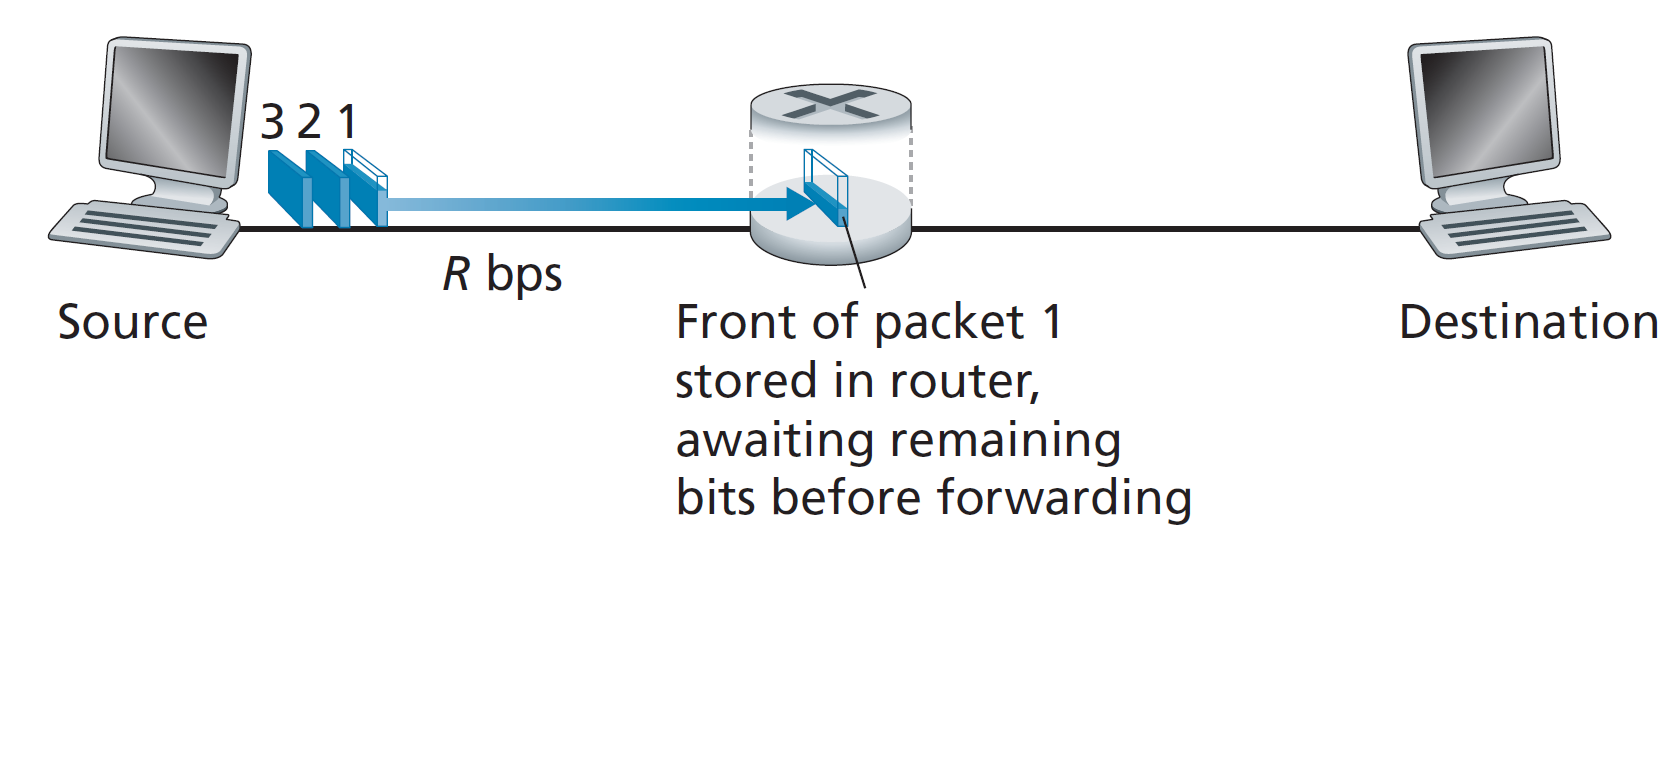
\includegraphics[keepaspectratio, width=12cm, height=9cm]{imagens/08/08 - store-and-forwarding.png}
\caption{Store and Fowarding \\
Imagem retirada de: Computer Networking a top-down approach. 8th
ed.~Pearson. Página 24. \\}
\label{fig:Store and Fowarding}
\end{figure}



Considerando L = 10 kbits e R = 100 Mbps, então L/P = 0.1 milissegundos.

Em casos reais, o cálculo do atraso total deve levar em conta, além do
\emph{transmission delay} (que está relacionado com o tempo necessário
para o dispositivo enviar os dados), outros tipos de atraso como no
processamento, atraso de enfileiramento e de propagação (que está
relacionado com o atraso na propagação do bit através do meio de
transmissão, impactado, portanto, pela distância. É calculado pela
divisão entre a distância e a velocidade de propagação). Deve-se
destacar que diferentes dispositivos irão fornecer distintas taxas de
transmissão e meios de propagação, algo que pode gear um gargalo no
sistema (afetando seu desempenho geral).

É importante perceber que, por consequência do limite de memória RAM,
pode ocorrer uma insuficiência de espaço para o armazenamento e
enfileiramento dos dados para transmissão. Além disso, o padrão
\emph{store-fowarding} trás consigo todos os problemas inerentes da
arquitetura produtor-consumidor (por causa de sua equivalência). Assim,
pacotes podem ser ignorados caso a memória RAM seja utilizada em sua
totalidade (algo que envolve outros conceitos como qualidade de serviço
e prioridade de transmissão).

Outro desvantagem dessa arquitetura tem haver com o seu impacto no
atraso de enfileiramento, pois cada pacote recém chegado deve esperar
todos os que entraram anteriormente serem retirados da fila, e como a
chegada de pacotes ocorre de forma aleatória (ou imprevisível), não há
como determinar exatamente o tempo de enfileiramento. Porém, podemos
estimar a intensidade de tráfego (\emph{traffic intesity}) analisando a
média, em bits por segundos, dos pacotes que chegam (La), pela taxa de
transmissão (R). Desse modo, pode ocorrer 3 casos, no qual:

\begin{enumerate}
\def\labelenumi{\arabic{enumi}.}
\tightlist
\item
  La/R \textgreater{} 1: fila e atraso crescentes (e, consequentemente,
  pode haver um estouro na memória RAM, como explicado anteriormente.
  Dispositivo com capacidade inadequada).
\item
  La/R = 1: fila e atraso constantes.
\item
  La/R \textless{} 1: fila e atrasos decrescentes ou mínimos.
\end{enumerate}

\hypertarget{analogia-com-uma-caravana}{%
\subsection{Analogia com uma caravana}\label{analogia-com-uma-caravana}}

A diferença entre o atraso da transmissão e propagação pode ser melhor
entendido fazendo-se uma analogia com uma caravana. Imagine uma caravana
(pacote) de 10 carros (10 bits) que percorrem (propagam) em uma
velocidade de 100 km/h, com cada carro gastando 12 segundos (transmissão
= 1 carro / 12 segundos) com o serviço do pedágio (roteador). O próximo
pedágio está a uma distância de 100 km. Assim, o tempo total de percorrer
do primeiro pedágio até a chegada ao segundo vai ser a soma do tempo da
caravana ser processada pelo primeiro pedágio (10 carros / 1 carro / 12
segundos = 2 minutos de atraso na transmissão \emph{transmission delay})
mais o tempo necessário para percorrer a pista (100km / 100 km/h = 60
minutos), algo que resulta em 62 minutos.

\hypertarget{circuit-swiching}{%
\subsection{Circuit-swiching}\label{circuit-swiching}}

A alternativa ao \emph{packet-switching} é o \emph{circuit-switching}
(mostrado na Figura \ref{Circuit Switching}), no qual faz uma conexão direta (ou circuito)
entre os computadores comunicantes (\emph{end-to-end connection}), tendo
assim, como vantagem, a garantia de uma taxa de transmissão constante
(impossibilita que outros computadores interfiram nessa estabilidade). O
uso do circuito é fundamentado na multiplexação, que, por sua vez, pode
ser baseada no tempo, com o TDM (\emph{time-division multiplexing}),
método em que um \emph{frame} (período fixo de tempo) é fracionando em
\emph{slots} de tempo, com cada \emph{slot} sendo dedicado a uma conexão
específica (assim, em um \emph{frame} ocorre diversas comunicações
diferentes), ou na frequência, utilizando o FDM
(\emph{frequency-division multiplexing}), no qual as frenquências de
comunicação de um \emph{link} são divididas entre as conexões.


\begin{figure}[H]
\centering
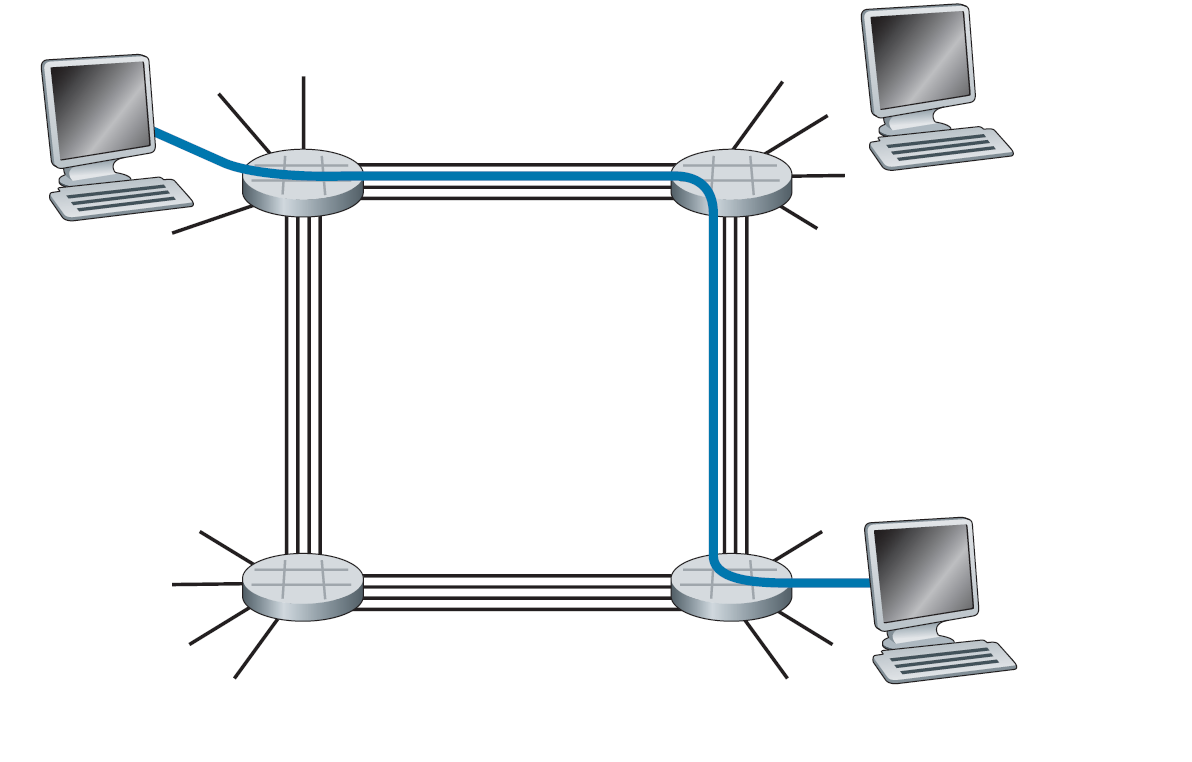
\includegraphics[keepaspectratio, width=12cm, height=9cm]{imagens/08/08 - circuit-switching.png}
\caption{Circuit Switching \\
Imagem retirada de: Computer Networking a top-down approach. 8th
ed.~Pearson. Página 28.\\}
\label{Circuit Switching}
\end{figure}

A desvantagem desse sistema é a ocorrência de ociosidade em períodos no
qual os computadores não estão se comunicando (\emph{silent periods}),
assim recursos de rede estão sendo alocados e não utilizados, portanto
desperdiçados. Outra inferioridade (comparado ao
\emph{packet-switching}) vem da complexidade de reservar uma capacidade
de transmissão ponta a ponta (\emph{end-to-end transmission}) e de
coordenar a sinalização relacionada com a multiplexação.




%\hypertarget{aula-9}{%
%\chapter{Aula: 9}\label{aula-9}}




\hypertarget{camada-de-aplicauxe7uxe3o-a-razuxe3o-de-existir-das-redes}{%
\chapter{Camada de Aplicação: a razão de existir das redes}\label{camada-de-aplicauxe7uxe3o-a-razuxe3o-de-existir-das-redes}}

A camada de aplicação (primeira camada) é considerada como a mais
importante, pois ela é quem gera a utilidade da rede. Assim, a
infraestrutura, bem como os protocolos, foram criados para servi-la, e,
portanto, sem a aplicação, não existiria as demais camadas. Essa
utilidade vem dos benefícios produzidos pela interação de dois processos
executados em computadores diferentes e, possivelmente, sistemas
operacionais diferentes. Para tal, há duas principais arquiteturas,
\emph{client-server} e \emph{peer-to-peer} (P2P).

\hypertarget{http}{%
\section{HTTP}\label{http}}

A arquitetura \emph{client-server} é empregue na aplicação \emph{Web}, o
qual usufrui do protocolo \emph{Hypertext Transfer Protocol} (HTTP).
Essa arquitetura funciona no sistema \emph{always on}, no qual o
servidor, ou processo que espera para ser contactado no início da
interação, deve sempre ficar ativo, e o seu endereço na rede fixado. Os
clientes não interagem diretamente entre si. O protocolo de transporte
usado é o TCP.

A escalabilidade dessa arquitetura (a capacidade de suportar o aumento
do número de clientes) está limitada pela capacidade da infraestrutura
já instalada. Assim, o aumento no número de \emph{requests} (derivado do
aumento no número de \emph{clients}) deve ser precedido por um aumento
na competência do servidor de lidar com os mesmos. Por essa razão, os
servidores são comumente hospedados em \emph{data centers}, algo que
facilita a escalabilidade, por alocar, dinamicamente, centenas de
dispositivos para o processo \emph{server} (o servidor se torna uma
entidade processada por múltiplos dispositivos).

O HTTP define a estrutura das mensagens e a forma que as mesmas são
trocadas. Essa troca é baseada no padrão \emph{response-request} (a
mensagem do \emph{client} é o \emph{request}, e a reposta do
\emph{server} o \emph{response}). O \emph{client} (uma navegador como o
\emph{Chrome}, por exemplo), definido por ser o processo que inicia a
comunicação, necessita do endereço do \emph{server}, chamado de URL, que
é composta por dois componentes, o \emph{hostname} (
\emph{http://www.google.com/}) e o \emph{pathname}
(\emph{/search?q=alguma+coisa}):

\begin{verbatim}
URL: http://www.google.com/search?q=alguma+coisa
\end{verbatim}

A mensagem HTTP \emph{request} segue o seguinte padrão:

\emph{Request Line}:
\texttt{GET\ /somedir/page.html\ HTTP/1.1\ \textbackslash{}r\textbackslash{}n}
(= Método + URL + HTTP \emph{version} + \emph{carriage return and line
feed})\\
\emph{Header lines} (line 1):
\texttt{HOST:\ www.google.com.br\ \textbackslash{}r\textbackslash{}n}
(\emph{host} no qual hospeda o objeto requisitado)\\
\emph{Header lines} (line 2):
\texttt{Connection:\ Mozilla/5.0\ \textbackslash{}r\textbackslash{}n}
(navegador \emph{Firefox})\\
\emph{Header lines} (line 3):
\texttt{Accept-language:\ fr\ \textbackslash{}r\textbackslash{}n}
(prefere a versão em língua francesa)\\
\emph{Header lines} (line x):
\texttt{...\ \textbackslash{}r\textbackslash{}n} (outras
configurações)\\
\emph{Entity body} (line y): \texttt{\textbackslash{}r\textbackslash{}n}
(pode ficar vazio, como no método \emph{GET}, ou preenchido, como no
método \emph{POST})

A mensagem HTTP \emph{response} segue o seguinte padrão:

\emph{Status Line}:
\texttt{HTTP/1.1\ 200\ OK\ \textbackslash{}r\textbackslash{}n} (Tudo
ocorreu bem)\\
\emph{Header lines} (line 1):
\texttt{Connection:\ close\ \textbackslash{}r\textbackslash{}n}
(\emph{server} irá encerrar a conexão)\\
\emph{Header lines} (line 2):
\texttt{Date:\ Tue,\ 18\ Aug\ 2015\ 15:44:04\ GMT\ \textbackslash{}r\textbackslash{}n}
(data em que o \emph{response} foi enviado)\\
\emph{Header lines} (line 3):
\texttt{Server:\ Apache/2.2.3\ \textbackslash{}r\textbackslash{}n} (nome
do servidor)\\
\emph{Header lines} (line 4):
\texttt{Last-Modified:\ Tue,\ 18\ Aud\ 2015\ 15:11:03\ GMT} (data da
última modificação)\\
\emph{Header lines} (line 5):
\texttt{Content-Length:\ 6821\ \textbackslash{}r\textbackslash{}n}
(número de bytes do objeto enviado - O mesmo está em \emph{Entity
body})\\
\emph{Header lines} (line 6):
\texttt{Content-Type:\ text/html\ \textbackslash{}r\textbackslash{}n}
(indica o formato do objeto, no caso uma página html)\\
\emph{Entity body} (line y):
\texttt{...\ \textbackslash{}r\textbackslash{}n} (dados do objeto)

\hypertarget{torrent}{%
\section{Torrent}\label{torrent}}

A segunda arquitetura citada anteriormente, a P2P, baseia-se na
inter-colaboração intermitente dos dispositivos na rede, ou \emph{peers},
de forma que esses podem ser \emph{client} e \emph{server}
simultaneamente (É importante perceber que, em uma sessão de comunicação
com um par de dispositivos, o \emph{client} é aquele que inicia o
contato e o \emph{server} aquele que espera para ser contactado, assim,
apesar de cada \emph{peer} assumir ambas as formas simultaneamente nessa
rede, elas tem um único papel para cada sessão). Essa arquitetura é
auto-escalável (\emph{self-escalability}), pois cada \emph{peer}, apesar
de adicionar novos \emph{requests}, adicionam também capacidade de
serviço na rede.

A popularidade desse protocolo vem do uso da tecnologia \emph{Torrent}.
Desenvolvida pela empresa \emph{BitTorrent}, essa tecnologia
descentraliza o fornecimento de arquivos, de forma que os \emph{peers},
conforme fazem o \emph{download}, também proporcionam os dados já
baixados de volta para a rede. Assim, a capacidade de transmissão não
está limitada pelo \emph{seed} (primeiro fornecedor de um conteúdo),
crescendo, e, consequentemente, tornando arquivos populares mais
acessíveis, conforme aumenta a participação dos usuários (sendo,
consequentemente, barato, por não necessitar a contratação de uma
infraestrutura para o fornecimento de arquivos).

Essa arquitetura enfrenta diversos desafios, como: segurança, performance
e confiabilidade.

\hypertarget{sockets}{%
\section{Sockets}\label{sockets}}

Os \emph{sockets} são uma estrutura de dados em \emph{kernel space}
(encontrados dentro do sistema operacional, ou seja, seu acesso é
através de uma chamada de sistema) que fornece (analogamente a uma
porta) uma interface (API, \emph{Application Programming Interface})
para a interação da camada de aplicação com a camada de transporte. Ele
se manifesta através de um FD (\emph{file descriptor}, um arquivo),
fornecendo um \emph{pipeline} para o processo (em \emph{user-space}).
Para ser executado, o \emph{socket} necessita do endereço do \emph{host}
(\emph{internet protocol address} ou \emph{IP address}) e do
identificador que especifica o processo receptor no \emph{host} (chamado
de \emph{Port Number}). Por padrão, o \emph{web server} utiliza a porta
80, e o \emph{mail server} (com o protocolo SMTP) é identificado pela
porta 25.

\hypertarget{serviuxe7os-de-transporte}{%
\section{Serviços de transporte}\label{serviuxe7os-de-transporte}}

Como citado anteriormente, a camada de transporte fornece uma série de
serviços para a camada superior. Esses serviços podem ser analisados sob
a ótica de: confiabilidade (\emph{reliable data transfer}), taxa de
transferência (\emph{throughput}), atraso (\emph{delay} ou \emph{timing})
e segurança (\emph{security}). Nesse sentido, a \emph{internet} prover
dois protocolos de transporte, o UDP e o TCP, os quais disponibiliza
serviços com características diferentes, de maneira que:

TCP:

\begin{enumerate}
\def\labelenumi{\arabic{enumi}.}
\tightlist
\item
  \emph{Handshaking procedure}: com uma preparação anterior ao envio da
  mensagem (confiabilidade).
\item
  \emph{Full duplex connection}: com os processos podendo receber e
  enviar dados.
\item
  \emph{Reliable data transfer service}: sendo os dados enviados sem
  erros e na ordem correta (confiabilidade).
\item
  \emph{Transport Layer Secutiry: uma melhora no TCP que fornece
  criptografia (}encryption\emph{), integridade de dados (}data
  integrity\emph{) e }end-point authentication* (segurança).
\item
  Garantia de entrega da mensagem.
\end{enumerate}

UDP (um \emph{lightweight transport protocol}):

\begin{enumerate}
\def\labelenumi{\arabic{enumi}.}
\tightlist
\item
  \emph{No handshaking procedure}: Não se sabe se o receptor está
  preparado para receber a mensagem.
\item
  \emph{Unreliable data transfer}: podendo ser recebidos dados
  corrompidos e fora de ordem.
\item
  Não há garantia de entrega da mensagem.
\item
  Rápida.
\end{enumerate}

É importante perceber que os serviços de \emph{timing} e
\emph{throughput}, apesar de serem necessários para algumas aplicações,
como \emph{internet telephony} (Skype), não são fornecidos pelos
protocolos de \emph{internet} atuais.

\hypertarget{complementar-3}{%
\section{Complementar}\label{complementar-3}}

\hypertarget{pesquisar-sobre-2}{%
\subsubsection{Pesquisar Sobre}\label{pesquisar-sobre-2}}

\begin{enumerate}
\def\labelenumi{\arabic{enumi}.}
\tightlist
\item
  \emph{Socket programming}: página 152 do livro \emph{Computer
  Networking a top-down approach 8th ed.}
\item
  \emph{Dual Stack}: IPv4 e IPv6
\item
  NAT
\item
  WireShark: www.wireshark.org
\item
  ip addr shwo
\item
  ip config /on
\item
  telnet 127.0.0.1 3000
\item
  SS - apt \textbar{} grep 3000
\item
  SS - apt \textbar{} grep telnet
\item
  nc - V - U 127.0.0.1 1200
\item
  ncat
\item
  CDN (\emph{Content Distribution Networks})
\item
  DASH (\emph{Dynamic Adaptive Streaming over HTTP}).
\item
  DNS (\emph{domain name system}): The Internet's Directory Service
\item
  telnet serverName 25
\item
  SMTP (\emph{Simple Mail Transfer Protocol})
\item
  \emph{Cookies} (\emph{User interaction})
\end{enumerate}


%\hypertarget{aula-10}{%
%\chapter{Aula: 10}\label{aula-10}}





\hypertarget{dns-domain-name-system}{%
\chapter{DNS: Domain Name System}\label{dns-domain-name-system}}

Quando um usuário acessa um \emph{site} na Internet, o mesmo digita um
nome, por exemplo:

\texttt{www.google.com.br}

Sabendo que o sistema de endereçamento utilizado é baseado no TCP/IP,
como o navegador é capaz de converter o nome digitado no endereço de IP
(\emph{Internet Protocol}) do servidor requisitado ?

Essa tradução é feita pelo \emph{Domain Name System} (DNS).

O DNS é um protocolo executado na camada de aplicação, que roda em UDP
(usando a porta 53), no qual fornece o serviço de tradução de
\emph{hostnames} (nome dos servidores) em IP \emph{address}. Seu
funcionamento é baseado em um sistema de banco de dados distribuídos
implementado em uma hierarquia de servidores.

Essa arquitetura adotada, em contraste com o \emph{design} centralizado,
foi escolhida por evitar:

\begin{enumerate}
\def\labelenumi{\arabic{enumi}.}
\tightlist
\item
  Único ponto de falha
\item
  Volume de tráfego
\item
  Manutenção
\item
  Distância do usuário (tempo de resposta)
\item
  Baixa escalabilidade
\end{enumerate}

\hypertarget{hierarquia-e-funcionamento}{%
\section{Hierarquia e funcionamento}\label{hierarquia-e-funcionamento}}

A hierarquia de servidores de DNS é composta por:

\begin{enumerate}
\def\labelenumi{\arabic{enumi}.}
\setcounter{enumi}{-1}
\tightlist
\item
  \emph{Local}: Não pertence a hierarquia, mas é de suma importância. É
  proporcionado pelo \emph{Internet Service Provider} (ISP)
\item
  \emph{Root}: cópia de 13 servidores, gerenciados por 12 diferentes
  organizações, e coordenado pela \emph{Internet Assigned Numbers
  Authority} (IANA)
\item
  \emph{top-level domain} (TLD): fornece o IP \emph{address} para os
  \emph{authoratives servers}. É mantido por diferentes empresas, como o
  Verisign Global Registry (\emph{.com}) e Educause (\emph{.edu})
\item
  \emph{Authoritative}: toda organização com acesso público deve prover
  servidores DNS (que pode ser mantido por eles ou por terceiros), com o
  \emph{primary} sendo o servidor principal e o \emph{secondary} o de
  \emph{backup}.
\end{enumerate}

Voltando ao exemplo do \texttt{www.google.com.br}, quando um usuário
digita esse \emph{hostname} e aperta enter, o navegador (\emph{browser})
gera uma uma estrutura de dados, chamada de DNS \emph{query}
\emph{message} (ou mensagem de consulta DNS), com uma série de
informações, como o nome \texttt{www.google.com.br} (\emph{hostname}),
que serão enviadas para o \emph{local} DNS \emph{server}.

A partir do \emph{local} DNS \emph{server}, pode ocorrer duas formas de
interação: recursiva e iterativa.

\hypertarget{iterativa}{%
\subsubsection{Iterativa}\label{iterativa}}

No modelo iterativo, o \emph{local server} envia um \emph{request} para
cada um dos servidores da hierarquia, como mostrado na Figura \ref{Modelo Iterativo}:

\begin{enumerate}
\def\labelenumi{\arabic{enumi}.}
\tightlist
\item
  Usuário: \emph{request} para \emph{local server}
\item
  \emph{local server}: \emph{request} para o \emph{Root server}
\item
  \emph{local server}: \emph{response} do \emph{Root server}
\item
  \emph{local server}: \emph{request} para o TLD \emph{server}
\item
  \emph{local server}: \emph{response} do TLD \emph{server}
\item
  \emph{local server}: \emph{request} para o \emph{Authorative server}
\item
  \emph{local server}: \emph{response} do \emph{Authorative server}
\item
  Usuário: \emph{response} do \emph{local server}
\end{enumerate}


\begin{figure}[H]
\centering
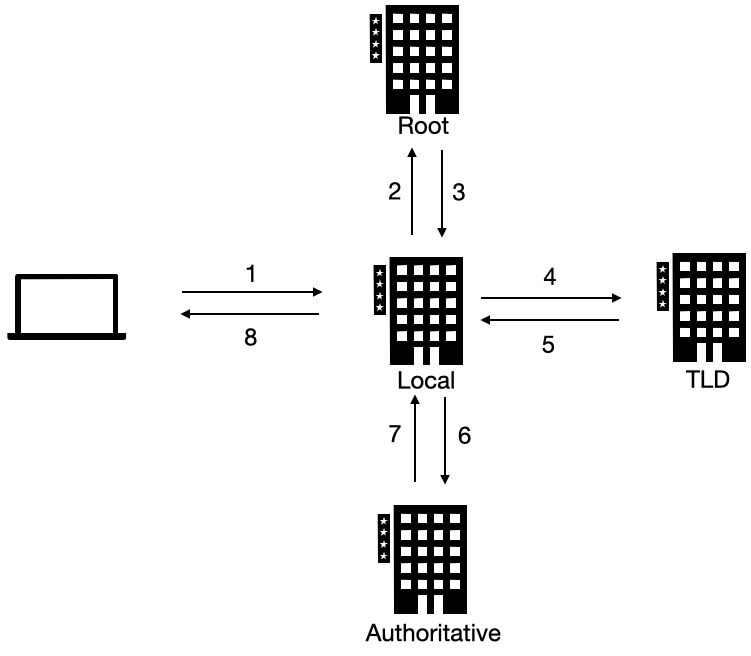
\includegraphics[keepaspectratio, width=12cm, height=9cm]{imagens/10/10 - modelo iterativo.png}
\caption{Modelo Iterativo \\}
\label{Modelo Iterativo}
\end{figure}



\hypertarget{recursivo}{%
\subsubsection{Recursivo}\label{recursivo}}

No modelo recursivo, mostrado na Figura \ref{Modelo Recursivo}, a sequência de \emph{requests} ocorrem em cadeia
entre os servidores:

\begin{enumerate}
\def\labelenumi{\arabic{enumi}.}
\tightlist
\item
  Usuário: \emph{request} para o \emph{local server}
\item
  \emph{Local server}: \emph{request} para \emph{root server}
\item
  \emph{Root server}: \emph{request} para TLD \emph{server}
\item
  TLD \emph{server}: \emph{request} para \emph{Authorative server}
\item
  TLD \emph{server}: \emph{response} do \emph{Authorative server}
\item
  \emph{Root server}: \emph{response} do TLD \emph{server}
\item
  \emph{Local server}: \emph{response} do \emph{root server}
\item
  Usuário: \emph{response} do \emph{local server}
\end{enumerate}


\begin{figure}[H]
\centering
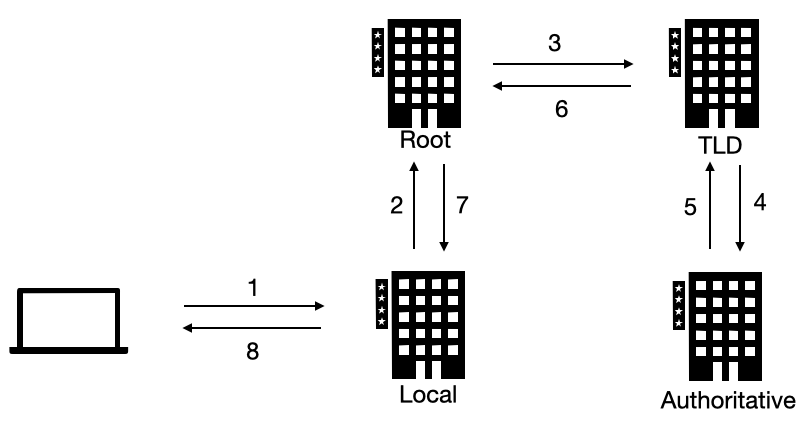
\includegraphics[keepaspectratio, width=12cm, height=9cm]{imagens/10/10 - modelo recursivo.png}
\caption{Modelo Recursivo \\}
\label{Modelo Recursivo}
\end{figure}



\hypertarget{dns-caching}{%
\section{DNS caching}\label{dns-caching}}

Nos dois modelos apresentados anteriormente, foi necessário 8 DNS
\emph{query messages} para a execução do serviço de tradução de
\emph{hostname} para IP \emph{address} (esse número pode ser maior, caso
houver \emph{Authorative servers} intermediários). Porém, de forma a
minimizar os impactos de tantas requisições, o \emph{local server}
utiliza um sistema de armazenamento temporário (pois o mapeamento entre
\emph{hostname} e IP \emph{address} não é permanente, alterando-se com o
tempo) da tradução, fazendo com o número de DNS \emph{query messages}
caia para apenas 2, o \emph{request} e o \emph{response} entre o usuário
e o \emph{local server}.

\hypertarget{vulnerabilidades}{%
\section{Vulnerabilidades}\label{vulnerabilidades}}

O DNS pode ser visto como um multiplicador de requisições, transformando
1, originada do usuário, em 8, que ocorrem entre os servidores do DNS,
algo que o torna especialmente vulnerável à ataques do tipo
\emph{Distributed Denial of Service} (DDoS). Para evitar tal fato, vem
sendo desenvolvido o DNSSEC (DNS \emph{Security Extensions}), uma versão
de segurança do DNS.

\hypertarget{resource-records}{%
\section{Resource Records}\label{resource-records}}

O DNS é um banco de dados distribuídos que armazena uma tupla de 4
elementos, \emph{Name}, \emph{Value}, \emph{Type} e \emph{time to live}
(TTL), o qual é utilizado para prover, entre outros, o mapeamento do
\emph{hostname} para IP \emph{address}. O dado armazenado em cada um dos
2 primeiros elementos citados da tupla variam conforme o \emph{type}. O
último elemento especifica quando o \emph{resource record} deve ser
removido do \emph{cache}.

A seguir será mostrado os dados contidos em \emph{Name} e \emph{Value}
para cada caso de \emph{Type} (os exemplos mostrados não contém o TTL).

\texttt{tupla\ =\ (name,\ value,\ type,\ ttl)}

\emph{Type} A\\
\emph{Name} = \emph{hostname}, \emph{Value} = IP \emph{address}\\
Tupla: \texttt{(relay1.bar.foo.com,\ 145.37.93.126,\ A)}

\emph{Type} NS\\
\emph{Name} = \emph{domain}, \emph{Value} = \emph{Authorative hostname
server}\\
Tupla: \texttt{(foo.com,\ dns.foo.com,\ NS)}

\emph{Type CNAME}\\
\emph{Name} = apelido (\emph{alias}) para \emph{hostname} , \emph{Value}
= \emph{hostname}\\
Tupla: \texttt{(foo.com,\ relay1.bar.foo.com,\ CNAME)}

\emph{Type MX}\\
\emph{Name} = apelido (\emph{alias}) do \emph{mail hostname},
\emph{Value} = \emph{mail hostname}\\
Tupla: \texttt{(foo.com,\ mail.bar.foo.com,\ MX)}


\hypertarget{dns-messages}{%
\subsubsection{\texorpdfstring{DNS
\emph{Messages}}{DNS Messages}}\label{dns-messages}}



O formato da mensagem DNS é mostrado na Figura \ref{Formato do DNS message}, segue a seguinte
estrutura:

\begin{figure}[H]
\centering
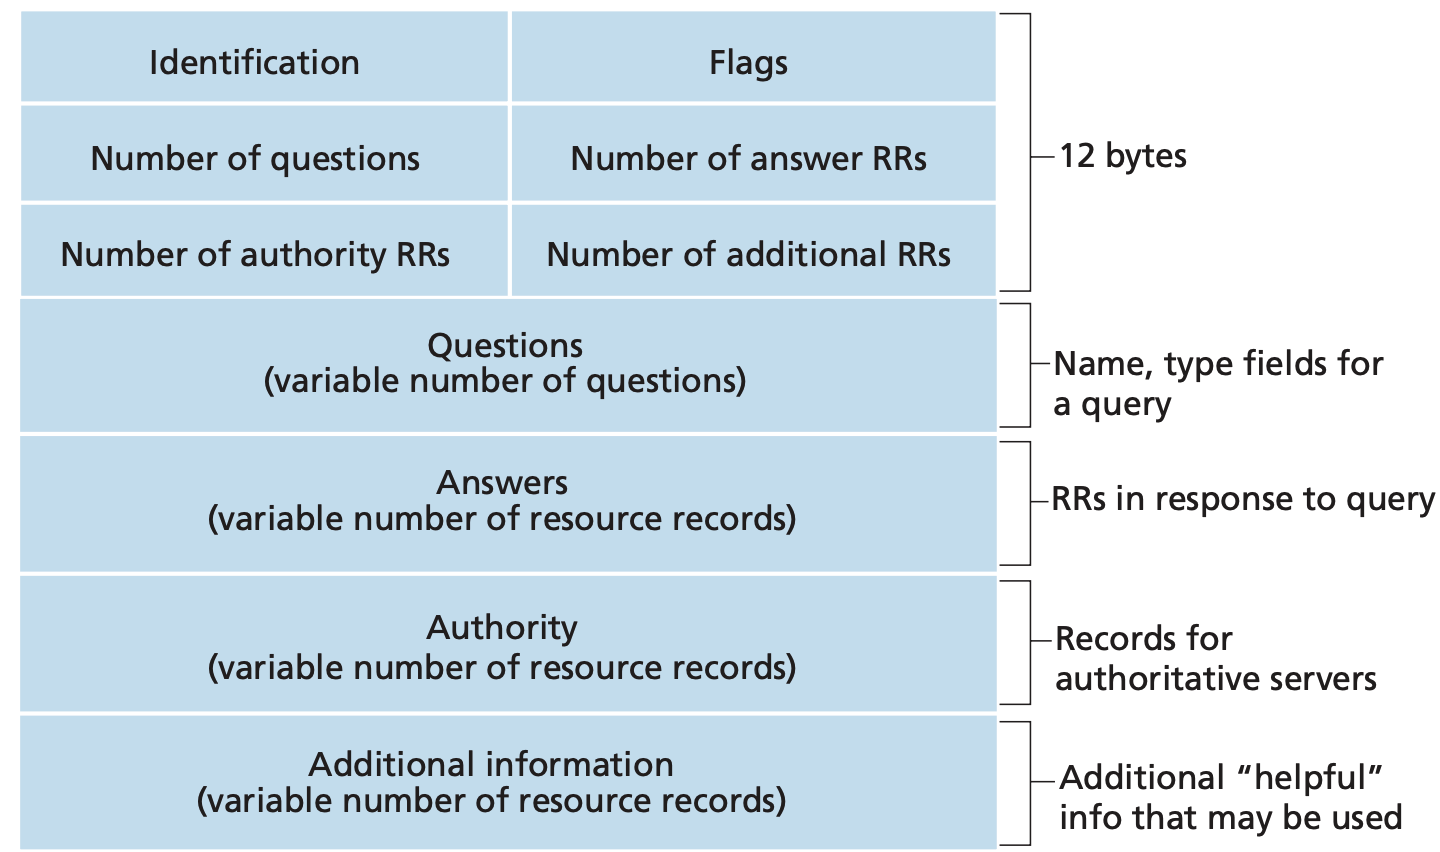
\includegraphics[keepaspectratio, width=12cm, height=9cm]{imagens/10/10 - DNS message format.png}
\caption{Formato do DNS message\\}
\label{Formato do DNS message}
\end{figure}


\begin{enumerate}
\def\labelenumi{\arabic{enumi}.}
\tightlist
\item
  Identificador: número de 16 bits que identifica a \emph{query}
\item
  Flags: cada flag é um indicador de 1 bit, no qual:\\
  2.1. \emph{query}/\emph{reply}: indica se é uma \emph{query} (0) ou um
  \emph{reply} (1)\\
  2.2. \emph{authoritative flag}: indica se o \emph{response} vem de um
  \emph{authorative server}\\
  2.3. \emph{recursion-desire}: indica o desejo do modelo recursão para
  as requisições (como mostrado anteriormente)\\
  2.4. \emph{recursion-available field}: ajustado na resposta, indica se
  o DNS \emph{server} suporta recursão
\item
  \emph{Number fields}: cada campo indica o número de ocorrências de
  cada sessão de dados
\item
  \emph{Questions}: contém informações como: \emph{host address} e
  \emph{name}, para \emph{type} A.
\item
  \emph{Answers}: populado pelo DNS \emph{server}, contém os
  \emph{resource records} para o \emph{hostname} requisitado.
\item
  \emph{Authority}: \emph{records} de \emph{authority servers}
\item
  \emph{Additional information}: contém outras informações
  interessantes.
\end{enumerate}

\hypertarget{adicionando-rr-no-banco-de-dados-dns}{%
\paragraph{Adicionando RR no banco de dados
DNS}\label{adicionando-rr-no-banco-de-dados-dns}}

A verificação (de unicidade) e adição de um novo RR no DNS é feito
através de entidades comerciais chamadas de \emph{registrar}, as quais
são acreditadas pela \emph{Internet Assigned Names and Numbers} (ICANN).
Para a adição, é necessário prover o \emph{domain name}, por exemplo
\texttt{google.com.br}, e o endereço de IP do DNS primário e secundário.

\hypertarget{complementar-4}{%
\section{Complementar}\label{complementar-4}}

\hypertarget{pesquisar-sobre-3}{%
\subsection{Pesquisar Sobre}\label{pesquisar-sobre-3}}

\begin{enumerate}
\def\labelenumi{\arabic{enumi}.}
\tightlist
\item
  https://alexanderell.is/posts/rpc-from-scratch/
\item
  https://datatracker.ietf.org/doc/html/rfc/
\item
  DNS over HTTPS (DoH): https://datatracker.ietf.org/doc/html/rfc8484
\item
  DNS over TLS (DoT): https://datatracker.ietf.org/doc/html/rfc8310
\end{enumerate}

%\hypertarget{aula-11}{%
%\chapter{Aula: 11}\label{aula-11}}




\hypertarget{transport-layer}{%
\chapter{Transport-Layer} \label{transport-layer}}

O objetivo da camada de transporte (\emph{transport layer}), executada
nos dispositivos localizados nas pontas da comunicação, é estender as
funcionalidades da \emph{network layer} com a preparação e envio dos
dados transmitidos pelos diferentes \emph{sockets}, técnica chamada de
\texttt{multiplexação}, e o direcionamento do pacote recebido para o
\emph{socket} competente, procedimento chamado de
\texttt{demultiplexação}. Dessa maneira, do ponto de vista da aplicação,
a \emph{transport layer} provê uma comunicação lógica, como se os
processos estivessem interconectados diretamente {[}algo similar ocorre
na \emph{network layer}{]}. Porém os diferentes protocolos existentes
nessa camada podem fornecer serviços adicionais, como confiabilidade da
transferência dos dados e controle de congestionamento, ambos presentes
no protocolo TCP (\emph{Transmission Control Protocol}, ou Protocolo de
Controle de Transmissão) e não encontrados no UDP (\emph{User Datagram
Protocol}).

A \texttt{multiplexação} e \texttt{demultiplexação}, ambas demonstradas
graficamente na Figura \ref{Multiplexação e Demultiplexação}, são possíveis devido à estrutura de dados
\emph{4-tuple}, no qual está contido os endereços de IP da origem e do
destino, e os identificadores únicos de 16 \emph{bits}, chamado de porta
(\emph{port}), dos \emph{sockets} de origem e destino.


\begin{figure}[h!]
\centering
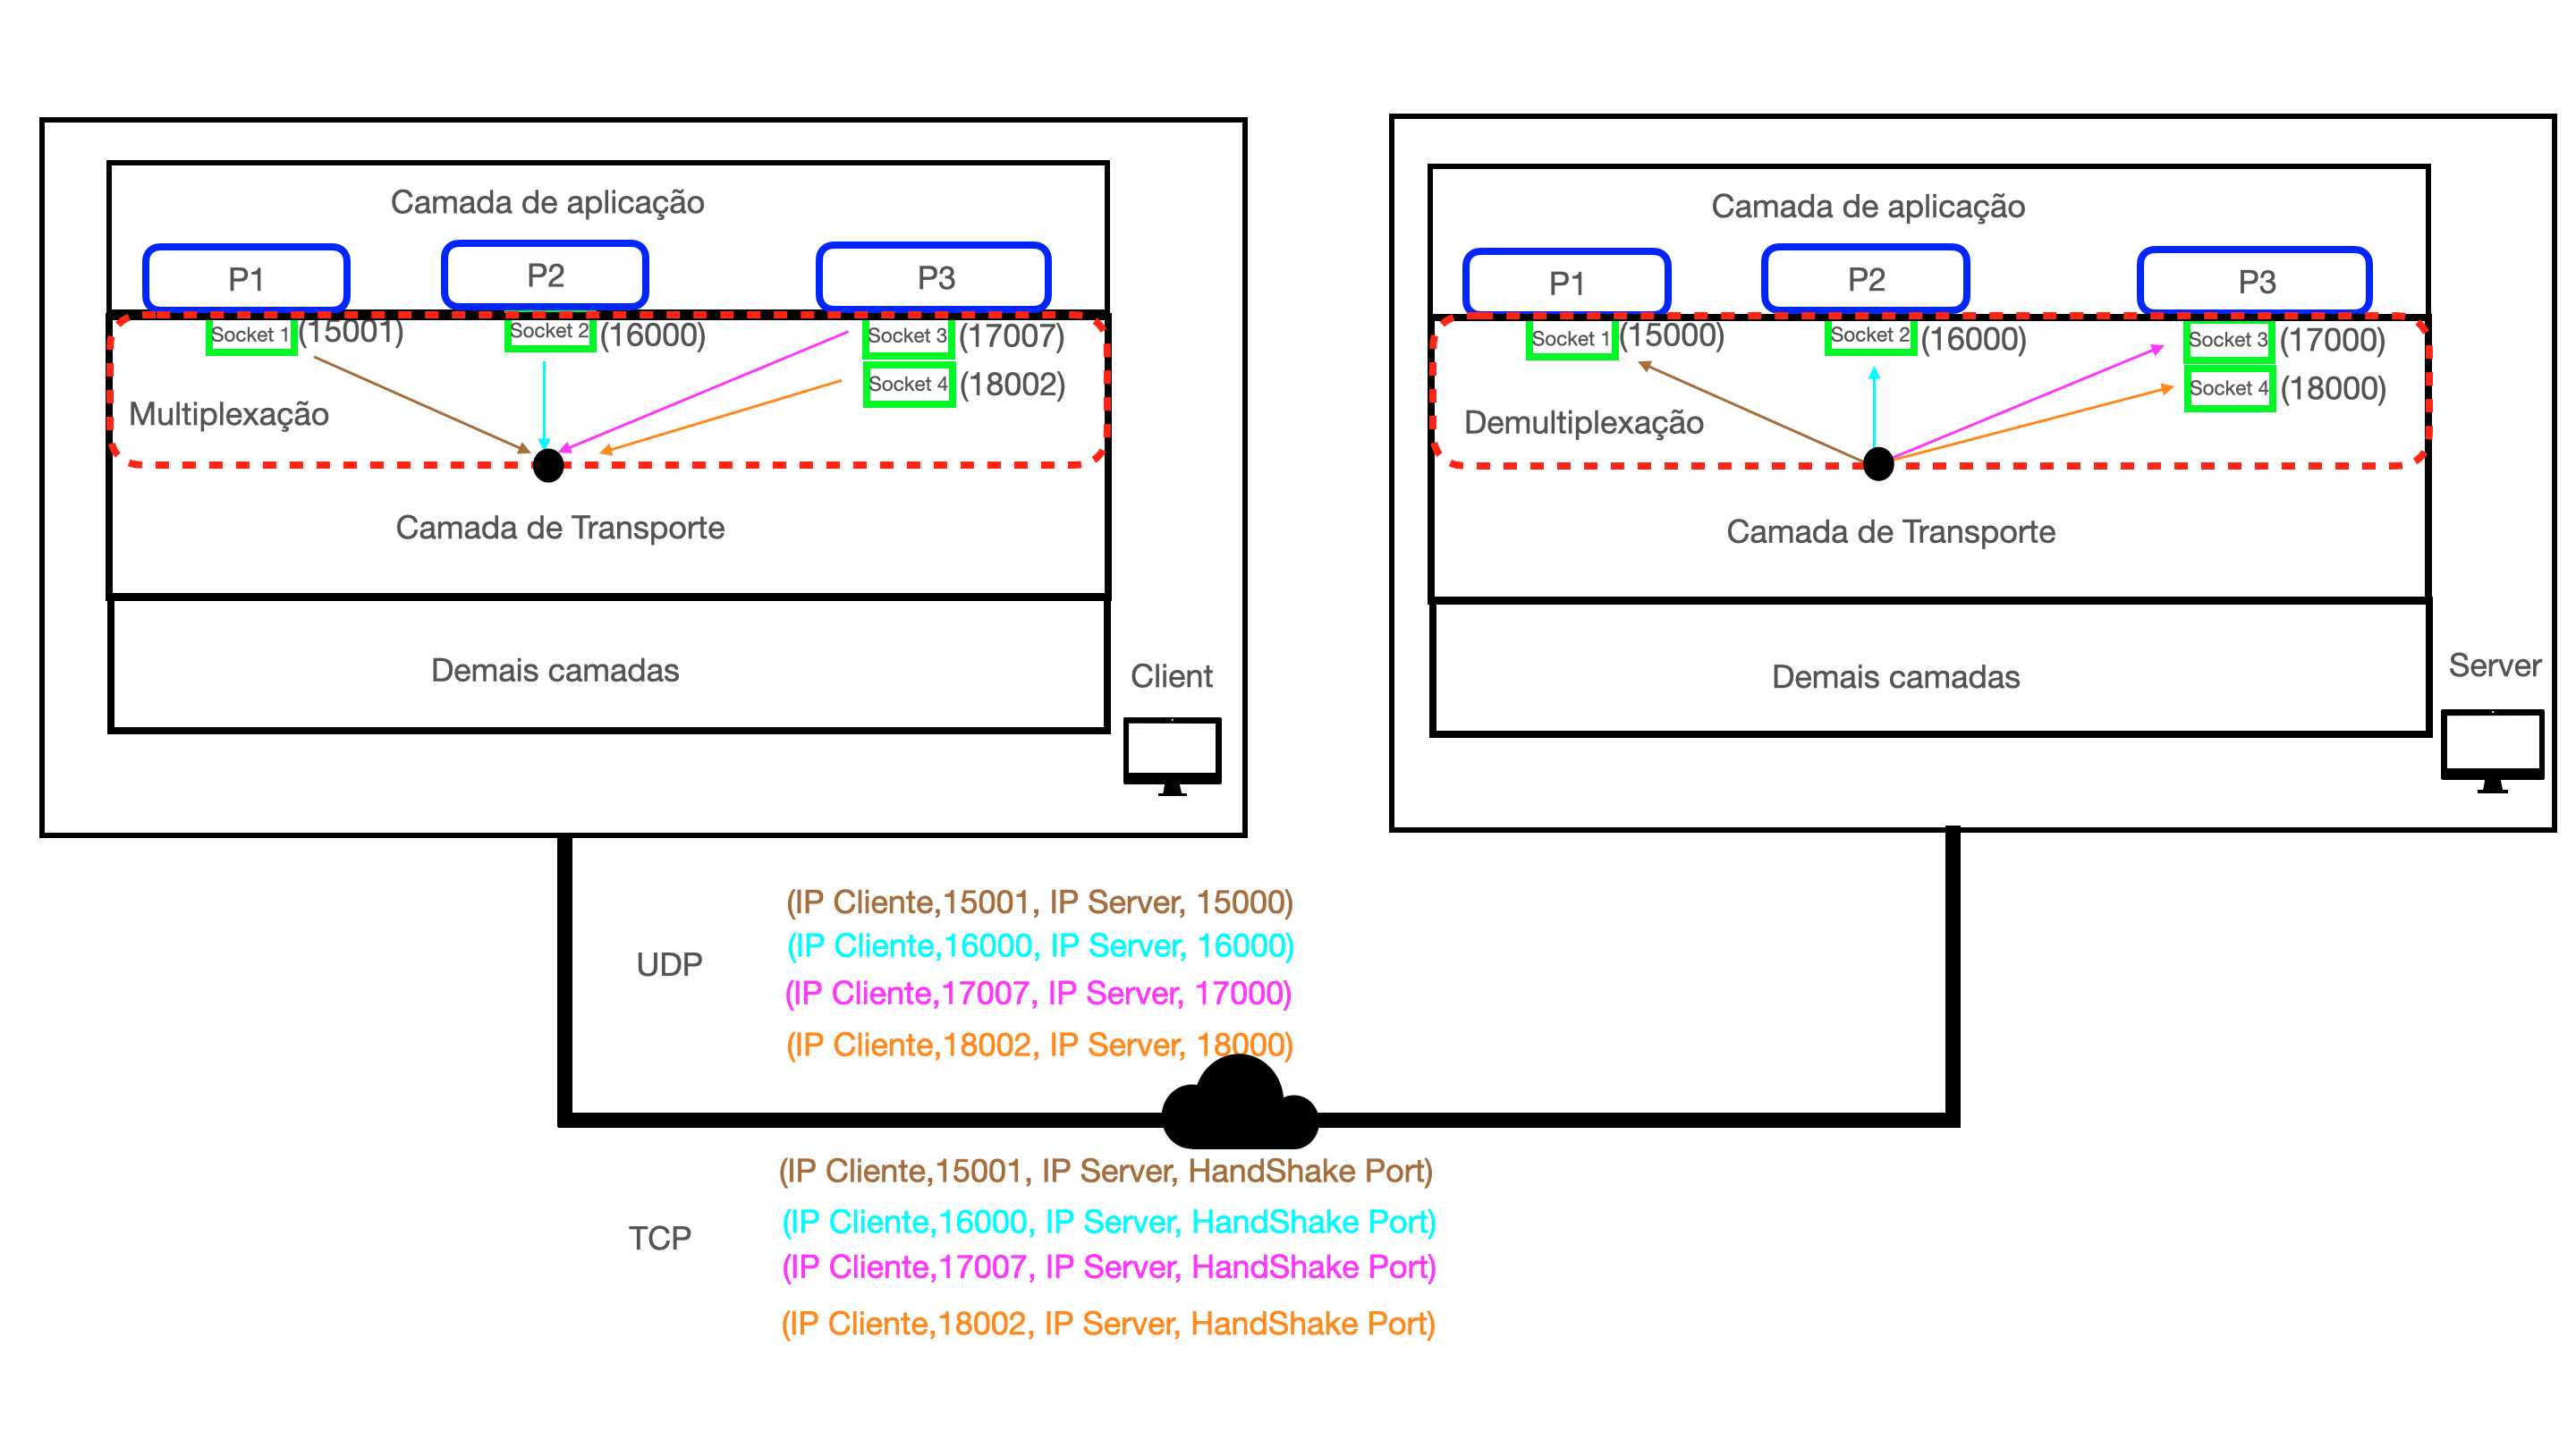
\includegraphics[keepaspectratio, width=16cm, height=12cm]{imagens/11/11 - Multiplexacao e Demultiplexacao.png}
\caption{Multiplexação e Demultiplexação\\}
\label{Multiplexação e Demultiplexação}
\end{figure}



Diferentemente do UDP, no qual a demultiplexação ocorre com o
encaminhamento dos dados diretamente para a porta de destino, descrita
no \emph{header} do \emph{segment}, (ou seja, o \emph{socket} UDP é
completamente identificável com \emph{2-tuple}, ou estrutura de dados
que contém o IP e \emph{port} de destino), o TCP necessita da
\emph{4-tuple} completa para a identificação do respectivo socket. Essa
abordagem simplifica a arquitetura \emph{client-server}, pois o servidor
pode utilizar de um única porta (como uma \emph{well-known port number},
número de porta que varia de 0 até 1023) para a execução do
\emph{handshaking}, como a 80 no caso do HTTP, enquanto que entrega
dinamismo à criação (ocorrendo no \emph{request}) e finalização dos
\emph{sockets}, algo que sucede o encerramento do canal de comunicação.
Na Figura \ref{Multiplexação e Demultiplexação} pode ser observado como os dados contidos na \emph{4-tuple}
podem variar conforme o protocolo escolhido.

É importante perceber que um processo pode ler e escrever no
\texttt{file\ descriptor} (\emph{socket}) criado para cada conexão
iniciada. E múltiplas conexões podem ser manipuladas por um único
processo, vinculando-se o \emph{socket} correspondente a uma thread
responsável pelo processamento das requisições do cliente. Desse modo,
um processo pode possuir múltiplos \emph{sockets} e interagir
individualmente com eles pelo \texttt{file\ descriptor} correspondente
na thread específica para a conexão em questão.

Dessa maneira, pode-se salientar uma forma de operação dos servidores,
no qual cada \emph{request} recebido gera um novo conjunto \emph{thread}
e \emph{socket} e o fim da conexão encerra esse conjunto. Portanto, o
período de vida do \emph{thread} e \emph{socket} pode ser longo, durando
toda a comunicação no modo persistente, ou curto, com a conexão
encerrando-se logo após o envio do \emph{response} no modo não
persistente. Requisições frequentes no modo não persistente podem
impactar no desempenho do sistema.

Como criar uma thread ou processo para cada requisição é
computacionalmente custoso, os \emph{servers} atuais implementam um
sistema produtor-consumidor, como mostrado na Figura \ref{Pool of Threads}, composto por
uma \emph{thread} produtora e um \emph{pool of threads} consumidoras. A
\emph{thread} produtora, vinculada à um \emph{socket}, recebe as
requisições oriundas dos \emph{clients} e deposita-os em uma fila
chamada \emph{task queue} (\emph{buffer}). Essas requisições serão
direcionadas para \emph{threads} consumidoras disponíveis, oriundas do
\emph{pool of threads}, as quais manterão-se ocupadas processando as
respectivas requisições coletadas (ou seja, não estarão disponíveis e,
portanto, não poderão adquirir novas requisições).

{[}Para saber mais, acesse:
https://httpd.apache.org/docs/2.4/mod/worker.html e
https://www.nginx.com/blog/thread-pools-boost-performance-9x/{]}


\begin{figure}[h!]
\centering
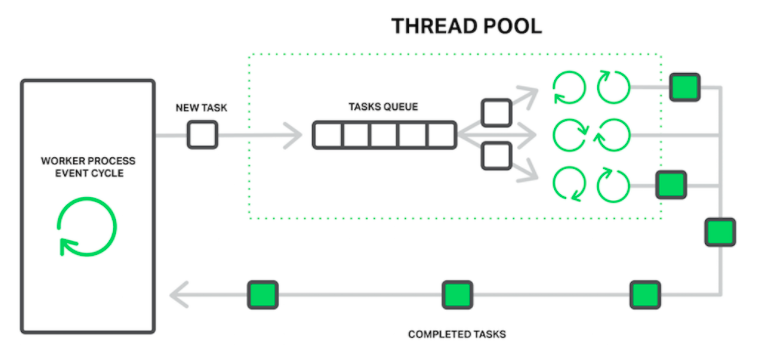
\includegraphics[keepaspectratio, width=12cm, height=9cm]{imagens/11/11 - pool of threads.png}
\caption{Pool of Threads \\
Imagem retirada de:
https://www.nginx.com/blog/thread-pools-boost-performance-9x/ em
05/12/2021. \\}
\label{Pool of Threads}
\end{figure}


\hypertarget{reliable-data-transfer-protocol}{%
\section {Reliable Data Transfer Protocol} \label{reliable-data-transfer-protocol}}

Para entender melhor sobre como funciona uma transferência de dados
confiável (\emph{Reliable Data Transfer Protocol}, RDT), será adotada
uma máquina computacional abstrada com um número finito de estados, no
qual assume somente um único estado por vez, chamada de Máquina de
Estados Finitos (\emph{Finite-State Machine}, FSM).

A cada nível de RDT será adicionado uma nova camada de complexidade, até
chegar no modelo mais próximo do real.

\hypertarget{rdt-1.0}{%
\subsection{RDT 1.0}\label{rdt-1.0}}

No primeiro caso, consideramos que as camadas mais baixas são
confiáveis. Ou seja não há perda ou alteração de dados e nem alteração
na ordem de envio. Assim:

Emissor:

\begin{enumerate}
\def\labelenumi{\arabic{enumi}.}

\item
  rdt\_send(data)
\item
  packet=make\_pkt(data)
\item
  udt\_send(packet)
\end{enumerate}

Receptor:

\begin{enumerate}
\def\labelenumi{\arabic{enumi}.}
\setcounter{enumi}{3}

\item
  rdt\_rcv(packet)
\item
  extract(packet,data)
\item
  deliver\_data(data)
\end{enumerate}

\hypertarget{rdt-2.0}{%
\subsection{RDT 2.0}\label{rdt-2.0}}

Em RDT 2.0, vamos considerar que, durante a transmissão, algum bit pode
ter sido corrompido. Assim, é necessário utilizar o protocolo ARQ
(\emph{Automatic Repeat reQuest}), o qual é baseado em três pontos:
detecção de erro, permitindo o receptor reconhecer a ocorrência de erro;
o \emph{feedback} do receptor, com o parecer positivo (equivalente à
``entendi!'') chamado de ACK ou negativo (equivalente à ``pode
repetir?''), denominado de NAK (em princípio, esse retorno basta ser de
1 bit de tamanho, sendo 0 para negativo e 1 para positivo); e
retrasmissão, com o emissor reenviando os pacotes caso tenha recebido
uma negativa (NAK) do receptor.

Emissor:

Envia os dados

\begin{enumerate}
\def\labelenumi{\arabic{enumi}.}
\tightlist
\item
  rdt\_send(data)
\item
  sndpkt = make\_pkt(data,checksum)
\item
  udt\_send(sndpkt)
\end{enumerate}

Espera por uma resposta\\
(reemissão em caso de NAK) 7. rdt\_rcv(rcvpkt) \&\& isNAK(rcvpkt)  \\
8. udt\_send(sndpkt)

(Encerra estado em caso de ACK)\\
9. rdt\_rcv(rcvpkt) \&\& isACK(rcvpkt)

Receptor: (Caso dados corrompidos)

\begin{enumerate}
\def\labelenumi{\arabic{enumi}.}
\setcounter{enumi}{3}
\tightlist
\item
  rdt\_rcv(rcvpkt) \&\& corrupt(rcvpkt)
\end{enumerate}

(Resposta)\\
5. sndpkt=make\_pkt(NAK) \\
6. udt\_send(sndpkt)

(Caso dados não-corrompidos)

\begin{enumerate}
\def\labelenumi{\arabic{enumi}.}
\setcounter{enumi}{3}
\tightlist
\item
  rdt\_rcv(rcvpkt) \&\& notcorrupt(rcvpkt)
\item
  extract(rcvpkt,data)
\item
  deliver\_data(data)
\end{enumerate}

(Resposta)\\
7. sndpkt = make\_pkt(ACK) 

8. udt\_send(sndpkt)

É importante perceber alguns detalhes desse protocolo. Primeiro, esse
protocolo é conhecido por \emph{stop-and-wait} pois o emissor não pode
receber nenhum comando do seu operador enquanto estiver esperando uma
resposta do receptor (novos comandos só correm quando a máquina estiver
em um estado apropriado). Segundo, não foi considerada a possibilidade
do ACK e NAK estarem corrompidos.

Para o segundo caso, há duas variações do RDT 2.0 no qual é implementado
um protocolo análogo ao incremento feito de RDT 1.0 para 2.0, chamados
de RDT 2.1 e 2.2.

\hypertarget{rdt-3.0}{%
\subsection{RDT 3.0}\label{rdt-3.0}}

Por fim, vamos considerar que poderá haver pacotes, ou suas respostas
ACK, perdidos durante a transmissão. A solução é o emissor esperar tempo
suficiente no qual garanta que os dados enviados ou respondidos foram
perdidos. Assim, caso o tempo seja ultrapassado, o emissor deve reenviar
os pacotes.

Como pode-se observar, não há como determinar um tempo ``garantidor'',
pois um atraso particularmente alto experimentado pelos pacotes pode ser
suficiente para ultrapassar o tempo estimado.

A determinação do tempo sofre de uma dicotomia, pois há vantagens e
desvantagens tanto com o aumento como com a diminuição do mesmo. Quanto
menor for o tempo, maior a chance de ocorrer falsas perdas (ocasionando
duplicações na emissão) por consequência de atrasos na rede. Porém,
incrementos nesse tempo podem impactar na velocidade da resposta do
emissor, pois o mesmo poderá ficar longos períodos de inatividade
aguardando uma resposta (perdida durante a transmissão). Assim, a
melhora na efetividade do protocolo passa pela determinação de um tempo
de espera ótimo (provavelmente desenvolvido para o atraso mais
frequente).

A Figura \ref{Protocolo RDT 3.0} mostra um exemplo do funcionamento do protocolo RDT 3.0
(também conhecido por \emph{alternating-bit protocol}, por causa da
alternância no número da sequência dos pacotes).

\begin{figure}[h!]
\centering
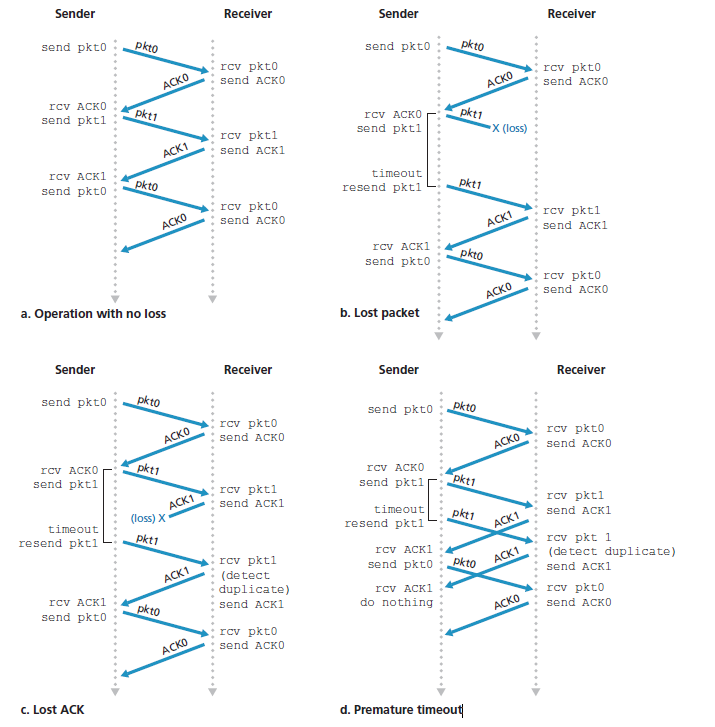
\includegraphics[keepaspectratio, width=14cm, height=17cm]{imagens/11/11 - rdt 3.0.png}
\caption{Protocolo RDT 3.0  \\
Imagem retirada de: Computer Networking a top-down approach. 8th
ed.~Pearson, página 212. \\}
\label{Protocolo RDT 3.0}
\end{figure}



\hypertarget{performance}{%
\subsection{Performance}\label{performace}}

O fundamento dos protocolos mencionados é enviar 1 pacote e esperar por
sua resposta. Uma forma de melhorar a performance é utilizar um padrão de
enviar múltiplos pacotes antes de entrar no estado de espera da resposta
de cada um, método chamado de \emph{pipeline}, como mostrado na Figura
\ref{Stop-and-wait vs pipelined}.


\begin{figure}[h!]
\centering
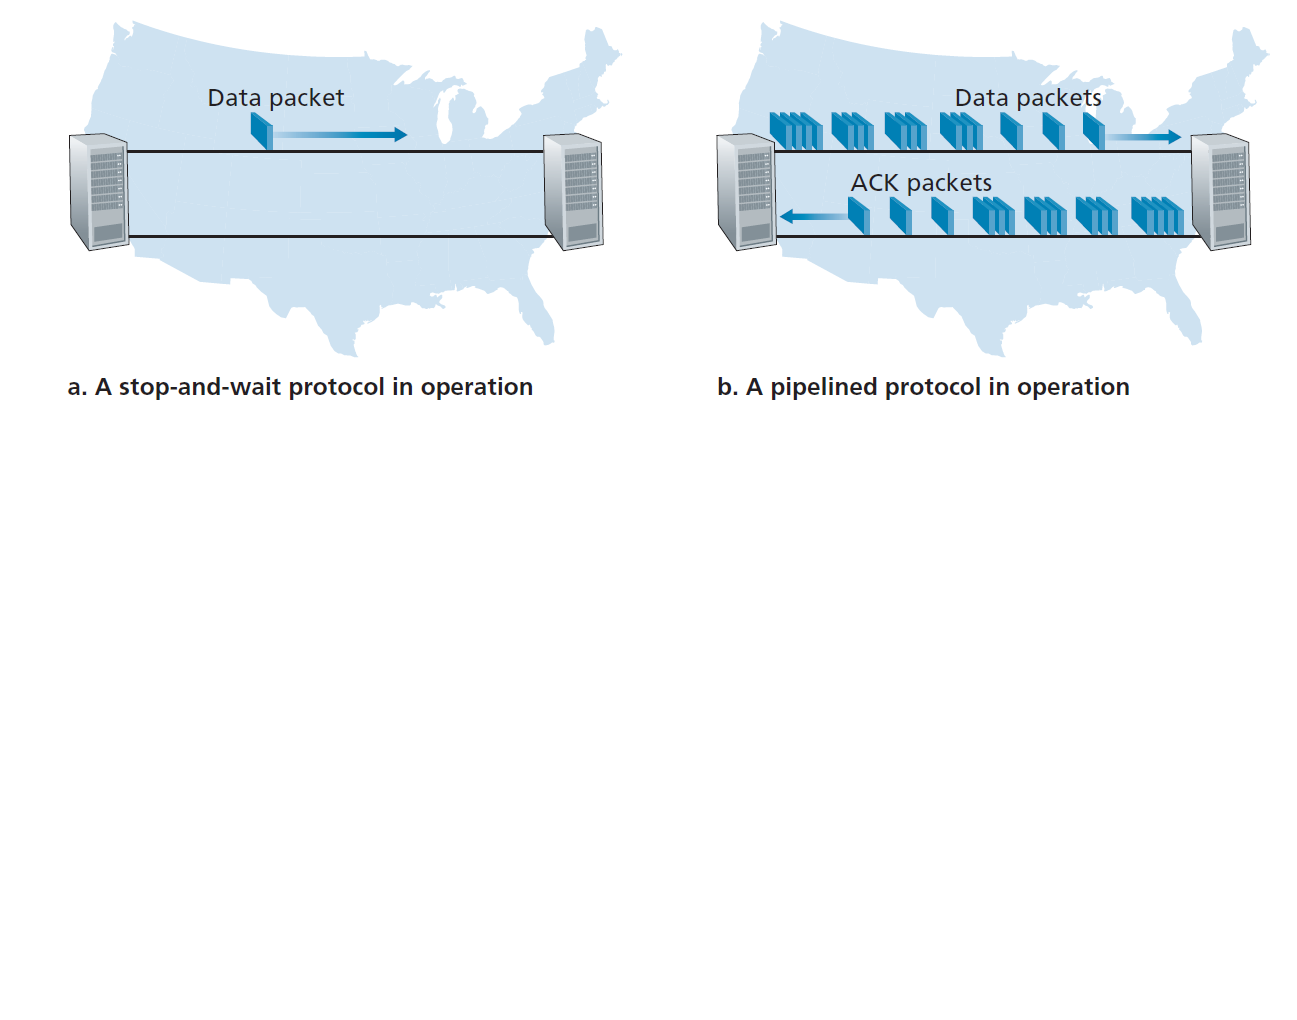
\includegraphics[keepaspectratio, width=14cm, height=11cm]{imagens/11/11 - stop and wait vs pipelined.png}
\caption{Stop-and-wait vs pipelined  \\
Imagem retirada de: Computer Networking a top-down approach. 8th
ed.~Pearson, página 213. \\}
\label{Stop-and-wait vs pipelined}
\end{figure}

Erros na abordagem do \emph{pipeline} são abordados nos protocolos
\emph{go-back-n} e \emph{selective repeat}, ambos tratados na próxima
aula.
%\hypertarget{aula-12}{%
%\chapter{Aula: 12}\label{aula-12}}




\hypertarget{continuauxe7uxe3o-transport-layer}{%
\chapter{Continuação: Transport Layer}\label{continuauxe7uxe3o-transport-layer}}

Como citado na aula anterior, o protocolo \emph{stop and wait}, no qual
o envio do próximo segmento (também é chamado de pacote por uma questão
histórica) ocorre somente após o recebimento da resposta do segmento
anterior, é uma forma ineficiente para a transferência de dados
confiáveis (\emph{reliable data transfer}, rdt) pois, após a transmissão
de um segmento, os recursos disponíveis para a conexão ficarão ociosos
até a chegada da resposta do segmento enviado. Dessa maneira,
objetivando o aumento da eficiência do mesmo, fora propostos duas
soluções: \emph{Go-Back-N} (GBN); e \emph{selective repeat}

\hypertarget{go-back-n}{%
\subsection{GO-BACK-N}\label{go-back-n}}

A ideia do protocolo GBN é baseado em um subconjunto de N elementos da
fila de transmissão (um dos motivos para a imposição de um tamanho
limite é o controle de fluxo). Os elementos dessa fila são compostos por
espaços que podem ser preenchidos por segmentos oriundo das camadas
superiores. Esse subconjunto, chamado de janela, contém os espaços
preenchidos por segmentos enviados mas sem confirmação
(\emph{acknowledged}) e espaços ainda não preenchidos. Ao receber uma
resposta, o espaço relacionado ao respectivo segmentos sai da janela, um
novo elemento da fila de transmissão é adicionado, gerando o efeito de
deslizar da janela para a direita na fila de transmissão. Devido a esse
efeito o GBN é chamado de \emph{sliding-window protocol}.

Caso todos os espaços disponibilizados pela janela estejam preenchidos,
novos dados não poderão ser aceitos, retornando às camadas superiores,
sendo esse retorno uma indicação de indisponibilidade.

Na metade superior da Figura \ref{Go-Back-N} podem ser reconhecidos os parâmetros:
\texttt{base}, que identifica o valor inicial incluído;
\texttt{nextseqnum}, referente ao próximo elemento a ser enviado; e
\texttt{send\ window\ size}, tamanho da janela (valor do N supracitado).
A metade inferior mostra o registro dos eventos ocorridos durante o
protocolo.

\begin{figure}[h!]
\centering
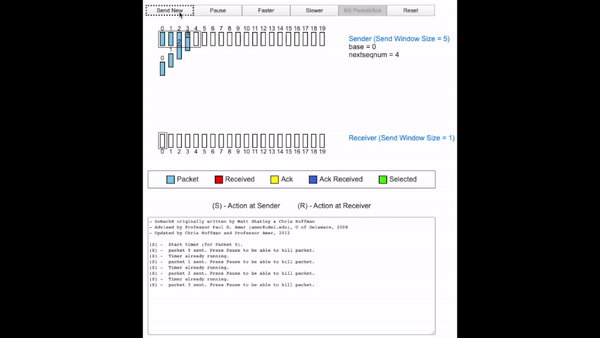
\includegraphics[keepaspectratio, width=12cm, height=9cm]{imagens/12/12 - GBN.png}
\caption{Go-Back-N \\
Disponível em:
https://media.pearsoncmg.com/aw/ecs\_kurose\_compnetwork\_7/cw/
content/interactiveanimations/go-back-n-protocol/index.html \\}
\label{Go-Back-N}
\end{figure}



Como o envio dos segmentos é feito em ordem, é esperado que os
respectivos ACK's sejam recebidos em ordem (\emph{cumulative
acknowledgment}). Caso o \emph{server} receba um segmento corrompido ou
fora de ordem, o mesmo é descartado e um ACK referente ao último
segmento íntegro ordenado é disparado. O ACK duplicado recebido é
descartado. Da perspectiva do \emph{client}, a não recepção ACK
correspondente ao segmento enviado, pode resultar em dois casos.
Primeiro, se a recepção do ACK `x + 1' ocorrer, porém a do `x' não, o
GBN considerará que o segmento `x' foi recebido corretamente pelo
\emph{server} e o seu ACK fora perdido durante a transmissão, marcando,
portanto, o segmento `x' como enviado corretamente. O segundo caso é a
respeito da não recepção de respostas dentro de um período
predeterminado (\emph{timeout}), algo que resulta na retransmissão dos
segmentos relativos.

Exemplo 1:

\begin{enumerate}
\def\labelenumi{\arabic{enumi}.}
\tightlist
\item
  \emph{cliente} dispara 5 segmentos (1, 2, 3, 4, 5)
\item
  \emph{server} recebe o segmento número 2 corrompido
\item
  \emph{server} dispara os seguintes ACK's: 1, 1, 1, 1, 1
\item
  \emph{cliente} recebe 5 ACK's referentes ao segmento 1, indicando a
  necessidade de retransmissão dos segmentos 2, 3, 4 e 5.
\end{enumerate}

Exemplo 2:

\begin{enumerate}
\def\labelenumi{\arabic{enumi}.}
\tightlist
\item
  \emph{client} dispara 5 segmentos (1, 2, 3, 4, 5)
\item
  \emph{server} recebe todos os segmentos corretamente
\item
  \emph{server} dispara os seguintes ACK's: 1, 2, 3, 4, 5
\item
  \emph{client} somente o ACK número 5, tendo, o resto, sido perdido
  durante a transmissão.
\item
  \emph{client} qualifica todos os 5 segmentos como tendo sido recebidos
  corretamente pelo \emph{server}
\end{enumerate}

\hypertarget{selective-repeat-sr}{%
\subsection{Selective Repeat (SR)}\label{selective-repeat-sr}}

É importante perceber, como mostrado no Exemplo 1, que um único elemento
corrompido pode causar a retransmissão de uma série de segmentos,
tornando, assim, o GBN ineficiente para esses casos. O aumento dessa
ineficiência é diretamente proporcional ao número de erros provocados
pelo canal de transmissão.

O protocolo \emph{Selective Repeat} (SR), como o próprio nome já induz,
tem o objetivo de diminuir o número de retransmissões desnecessárias.
Para tal, utiliza um subconjunto de N elementos da fila de transmissão,
chamada de janela, com cada elemento sendo um espaço que pode ser
preenchido por um segmento e marcado como não usável, usável, enviado e
confirmado, algo análogo ao GBN. Porém, diferencia-se pelo seu
comportamento, como mostrado na Figura \ref{Selective Repeat}.


\begin{figure}[h!]
\centering
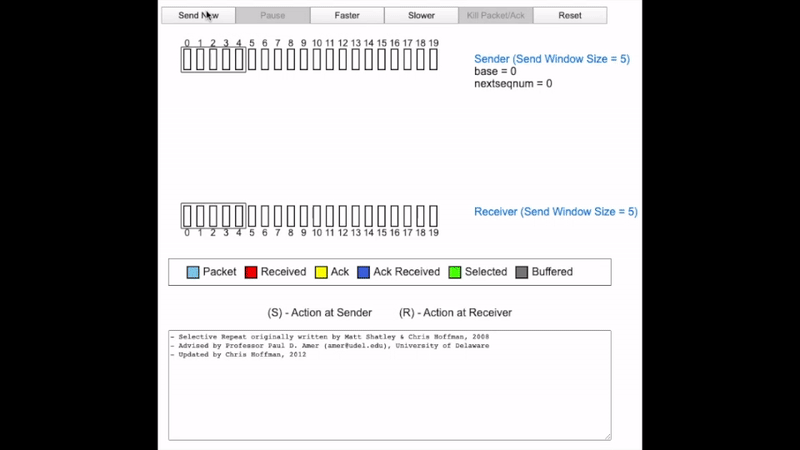
\includegraphics[keepaspectratio, width=12cm, height=9cm]{imagens/12/12 - animation of selective repeat.png}
\caption{Selective Repeat \\
Disponível em:
https://media.pearsoncmg.com/aw/ecs\_kurose\_compnetwork\_7/cw/content/interactiveanimations/selective-repeat-protocol/index.html \\}
\label{Selective Repeat}
\end{figure}



\begin{enumerate}
\def\labelenumi{\arabic{enumi}.}
\tightlist
\item
  um elemento só é marcado como confirmado quando o mesmo receber seu
  respectivo ACK.
\item
  a janela desloca-se somente após o recebimento do ACK relativo ao
  elemento na posição \texttt{base}, localizado no início da janela.
\item
  o \emph{server} enviará um ACK para cada segmento mesmo se ele estiver
  fora de ordem (mas dentro das condições citadas a seguir).
\item
  o \emph{client} terá uma janela própria (do mesmo tamanho da janela do
  \emph{client}), organizando-a, também, com 4 marcadores: esperado;
  fora de ordem; aceitado; não usável.
\item
  um segmento recebido fora de ordem não será descartado e sim
  armazenado em uma memória temporária (\emph{buffer}) (novamente,
  dentro das condições citadas a seguir).
\end{enumerate}

Esse comportamento gera uma possível dessincronização da posição das
janelas do \emph{cliente} e do \emph{server}, pois o \emph{server} pode
receber adequadamente um segmento mas o seu ACK relativo ter sido
corrompido ou perdido durante a transmissão. O pior caso de
dessincronização ocorre quando todos os ACK's enviados tenham sido
perdidos e, consequentemente, o \emph{server} estará adiantado em
\texttt{N} elementos. Assim, caso o \emph{server} receba um segmento com
o número da sequência entre entre os intervalos:



\begin{enumerate}
\def\labelenumi{\arabic{enumi}.}
\tightlist
\item
    \texttt{[`base`, `base` + `N` - 1]: armazenar em memória temporária e enviar o ACK.}
\item
    \texttt{[`base`-N, `base` - 1]: reenviar o ACK.}
\item
  Fora dos anteriores: ignorar.
\end{enumerate}

A dessincronização pode causar a recepção de um segmento já recebido,
gerando um dilema para o receptor: o segmento recebido é novo ou é uma
retransmissão ?

Essa possível dessincronização pode causar um dilema para o receptor dos
dados, pois, como mostrado na A Figura \ref{Dilema do Selective Repeat} mostra o dilema ocasionado
pela possível dessincronização: os dados recebidos são derivados de uma
retransmissão, como mostrado em (a), ou de um novo segmento (b)?

\begin{figure}[h!]
\centering
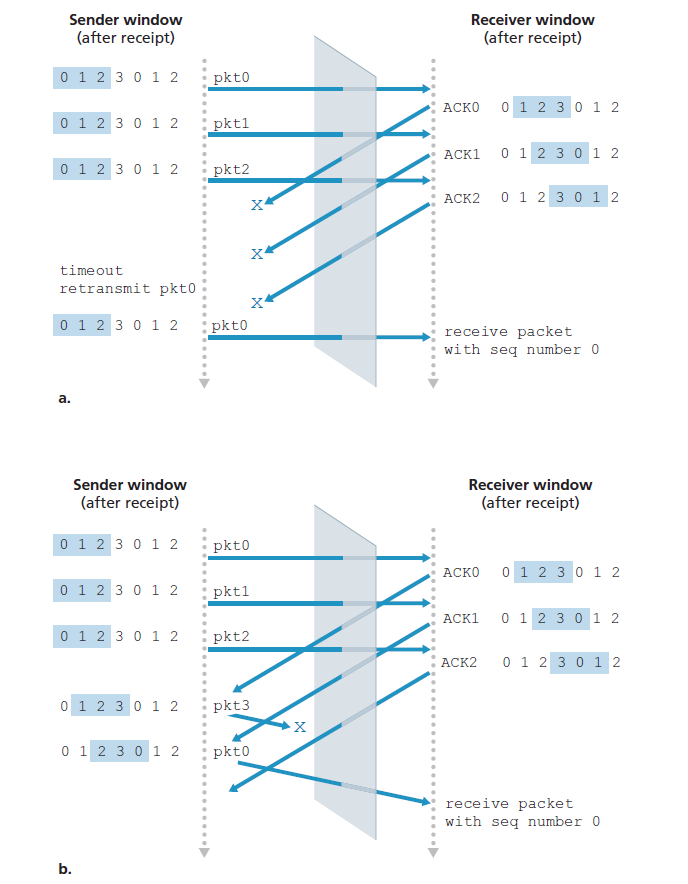
\includegraphics[keepaspectratio, width=18cm, height=15cm]{imagens/12/12 - Dilema do Selective Repeat.png}
\caption{Dilema do Selective Repeat \\
Imagem retirada de: Computer Networking a top-down approach. 8th
ed.~Pearson, página 225. \\}
\label{Dilema do Selective Repeat}
\end{figure}


Colocações importantes:

\begin{enumerate}
\def\labelenumi{\arabic{enumi}.}
\tightlist
\item
  O número de sequência é um valor finito determinado pelo número de
  bits disponibilizados para tal.
\item
  O \emph{buffer} do receptor deve poder armazenar 2 janelas, ou seja, o
  seu tamanho deve ser, no mínimo, o dobro do \texttt{window\ size}
  (\texttt{N}).
\item
  O \texttt{N} é determinado durante o \emph{handshaking}, limitado pelo
  tamanho do \emph{buffer} do receptor (como citado em 2).
\end{enumerate}

\hypertarget{tcp}{%
\subsection{TCP}\label{tcp}}

A camada de aplicação (\emph{application layer}), para o envio de um
arquivo, conta com os serviços de transmissão de dados confiáveis
fornecidos pelo \emph{Transmission Control Protocol} (TCP), protocolo da
camada de transporte. O TCP, ao receber o arquivo oriundo da
\emph{application layer}, divide-o em pedaços de comprimentos iguais
chamados de \emph{chunk's of data} (com exceção do último, normalmente
menor), de tamanho igual ao MSS (\emph{maximum segment size}),
normalmente de 1460 \emph{bytes}. O encapsulamento de um \emph{chunk of
data}, etapa que une o mesmo com o \emph{header} do TCP, resulta em um
conjunto de dados chamado de segmento.

O parâmetro MSS é determinado pelo MTU (\emph{Maximum Trasmission
Unit}), tamanho máximo do \emph{frame} da camada de enlace
(\emph{link-layer}), que tem como objetivo garantir que o segmento TCP
somado com o \emph{header} do TCP/IP (tipicamente 40 bytes), caberá no
\emph{frame} do \emph{link-layer}.

Após sua formação, o segmento é inserido no \emph{send buffer}, memória
temporária destinada ao envio dos dados para as camadas inferiores. Essa
memória é acessada de tempos em tempos para o envio dos segmentos ali
presentes.

Porém, diferente do UDP, o TCP é um protocolo orientado à conexão
(\emph{connection-oriented}), pois o primeiro contato entre dois
dispositivos ocorre com base no procedimento \emph{3-way handshake}, o
qual visa assegurar à confiabilidade na transmissão dos dados a partir
da definição dos parâmetros da conexão. O \emph{3-way handshake} é
caracterizado pela transmissão de 3 segmentos especiais. O primeiro é
emitido pelo \emph{client} visando o início da conexão. O segundo é uma
resposta do \emph{server}, indicando que o segmento foi recebido
corretamente. Por fim, o \emph{client} confirma que também recebeu o
segmento oriundo do \emph{server}. Os dois primeiros segmentos especiais
não contém dados, mas o terceiro pode conter.

A seguir está listado as características principais do TCP (mencionado
em aulas anteriores):

\begin{enumerate}
\def\labelenumi{\arabic{enumi}.}
\tightlist
\item
  Ponto-a-ponto
\item
  Transmissão de confiança, com fluxo de dados ordenado
\item
  \emph{Full Duplex}: fluxo de dados bi-direcional na mesma conexão
\item
  \emph{cumulative} ACK's
\item
  \emph{Pipelining}: controle de fluxo e congestionamento
\item
  \emph{Connection-oriented}
\item
  Fluxo controlado: o emissor não irá sobrecarregar o receptor
\end{enumerate}

\hypertarget{estrutura-do-segmento-tcp}{%
\subsubsection{Estrutura do segmento TCP}\label{estrutura-do-segmento-tcp}}

Como citado anteriormente, o segmento do TCP é composto por seu
\emph{header} e pelo pedaço do dado enviado pela camada de aplicação. O
\emph{header} é a sessão do segmento responsável pelos parâmetros de
conexão. São eles:

\begin{enumerate}
\def\labelenumi{\arabic{enumi}.}
\tightlist
\item
  números das portas de origem e destino, utilizados na multiplexação e
  demultiplexação, respectivamente.
\item
  \emph{checksum field}, importante na validação da integralidade dos
  dados recebidos
\item
  32-bit \emph{sequence number field}
\item
  32-bit \emph{acknowledgment number field}
\item
  16-bit \emph{receiver window}: usado para \emph{flow control}, indica
  o número de bytes que o receptor está disposto a aceitar
\item
  4-bit \emph{header length field}: especifica o tamanho do
  \emph{header} do TCP (como, normalmente, o \emph{options field} não é
  populado, o tamanho típico do \emph{header} é de 20 \emph{bytes})
\item
  \emph{options field}: é útil para a negociação do MSS entre outros.
\item
  \emph{flag field}: campo que contém 6 bits 8.1. bit ACK: indica a
  validade do campo ACK 8.2. bits RST, SYN e FIN: são usados para
  configuração das conexões 8.3. bits CWR e ECE: notificações de
  congestionamento 8.4. bit PSH: indica que o receptor deve repassar, de
  imediato, os dados recebidos para as camadas superiores 8.5. bit URG:
  marcado pela camada de aplicação do emissor, indica que há dados
  urgentes (Na prática, os bits PSH e URG não são usados)
\end{enumerate}

A Figura \ref{Estrutura do segmento TCP} mostra toda a estrutura do segmento TCP.


\begin{figure}[h!]
\centering
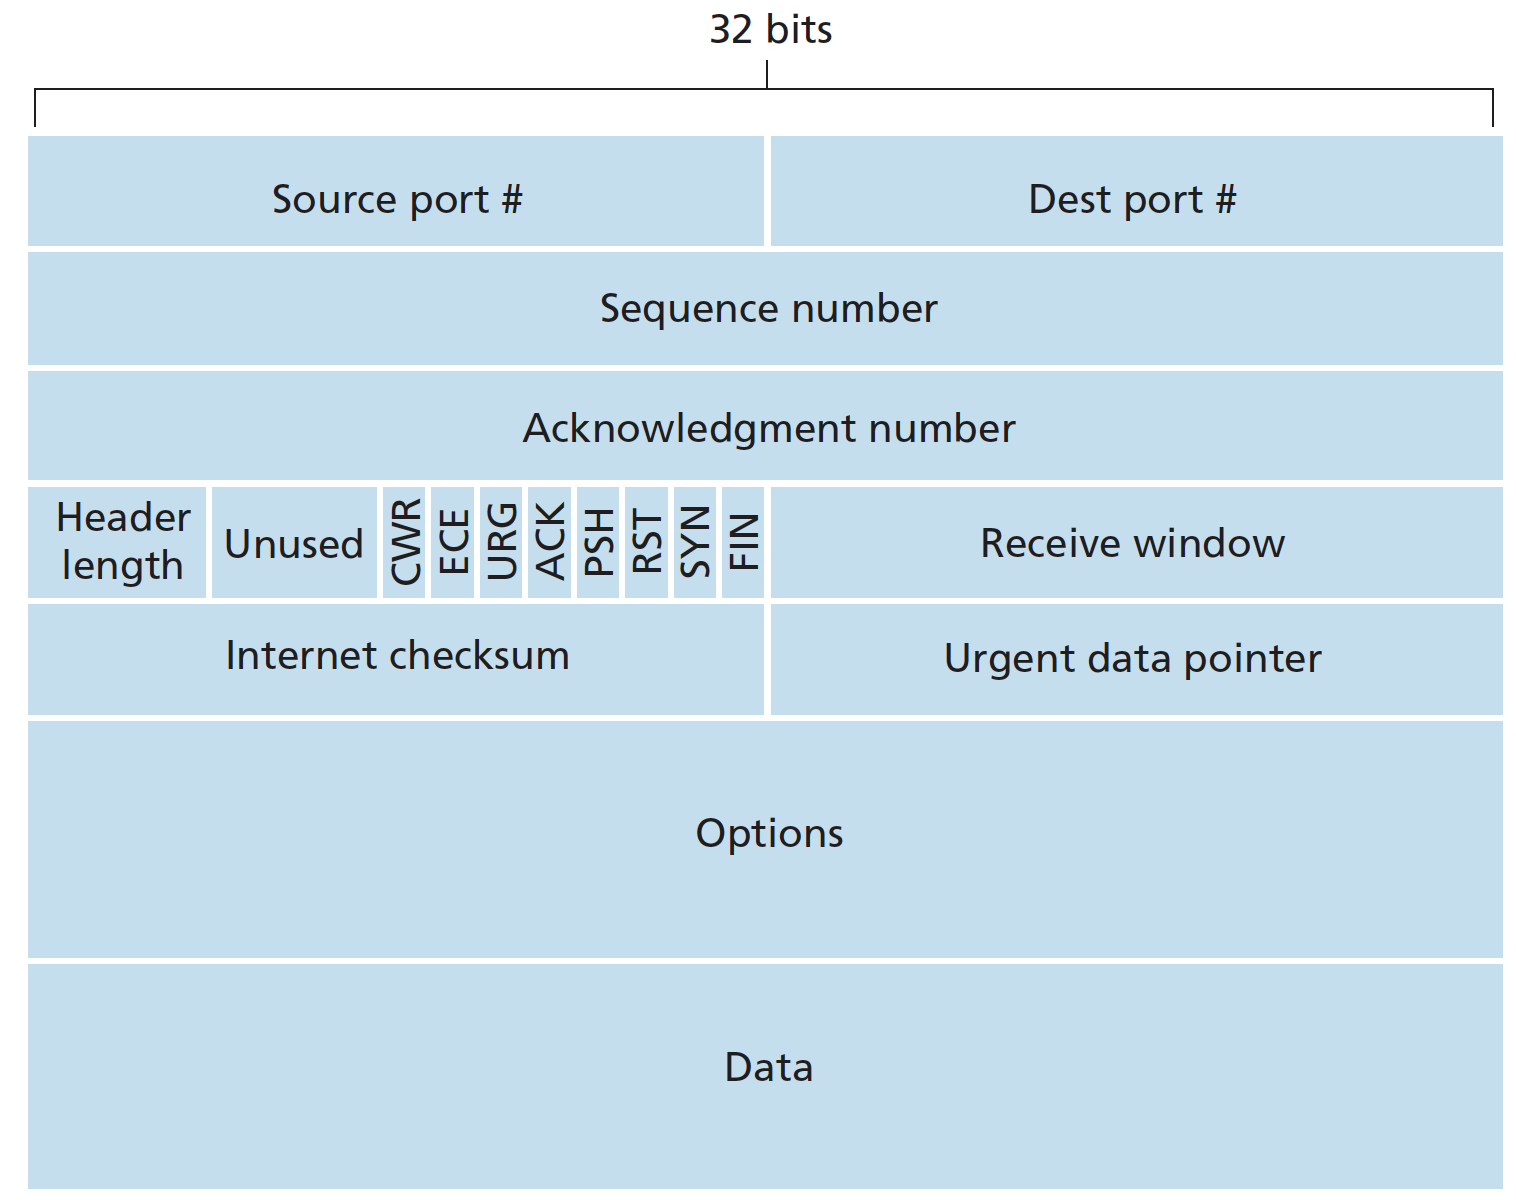
\includegraphics[keepaspectratio, width=12cm, height=9cm]{imagens/12/12 - Estrutura segmento TCP.png}
\caption{Estrutura do segmento TCP \\
Imagem retirada de: Computer Networking a top-down approach. 8th
ed.~Pearson, página 231. \\}
\label{Estrutura do segmento TCP}
\end{figure}



\hypertarget{sequuxeancia-e-ack}{%
\ssubsection{Sequência e ACK}\label{sequuxeancia-e-ack}}

O TCP vê os dados como um conjunto ordenado e não estruturado de fluxo
(\emph{stream}) de bytes, de forma que o \emph{sequence number} é uma
referência à ordem dos bytes (mais especificamente, a ordem do primeiro
\emph{byte} dos dados do segmento) e não da série de segmentos enviados.
Assim, para um arquivo de 500.000 \emph{bytes} (500 kB) e um MSS de
1.000 bytes (1 kB) serão construídos 500 segmentos, com o primeiro
assumindo o \emph{sequence number} de 0, o segundo 1000, o terceiro
2000, e assim em diante.

Já \emph{acknowledgment number} (ACK \emph{number}) é relativo ao
\emph{sequence number} do próximo \emph{byte}. Seguindo o exemplo
anterior, está contido, no primeiro segmento, 1000 bytes, e o seu
\emph{sequence number} é de 0 (portanto existem nesse segmento os
\emph{bytes} 0 até 999). Assim, após a chegada no \emph{byte} 999, o
receptor enviará a confirmação da recepção desse segmento com o
\emph{acknowledgment number} de 1000 (byte seguinte ao último recebido).
Dessa maneira, como o receptor só confirma (\emph{acknowledges}) o
primeiro byte ausente, no caso, o byte 1000, o protocolo TCP é dito como
provedor de \emph{cumulative acknowledgments}.

A Figura \ref{Sequence number e ACK} mostra um exemplo de como a variação do \emph{sequence number} e do \emph{acknowledgment number} ocorrem com o MSS de 1
\emph{byte} no Telnet. O \emph{Host A} envia seu \emph{byte} 42
(\emph{sequence number}) requisitando (ACK) o byte de \emph{sequence
number} 79 do \emph{Host B}, e o \emph{Host B} responde com o seu
\emph{byte} 79 e requisita o \emph{byte} 43 do \emph{Host A}.


\begin{figure}[h!]
\centering
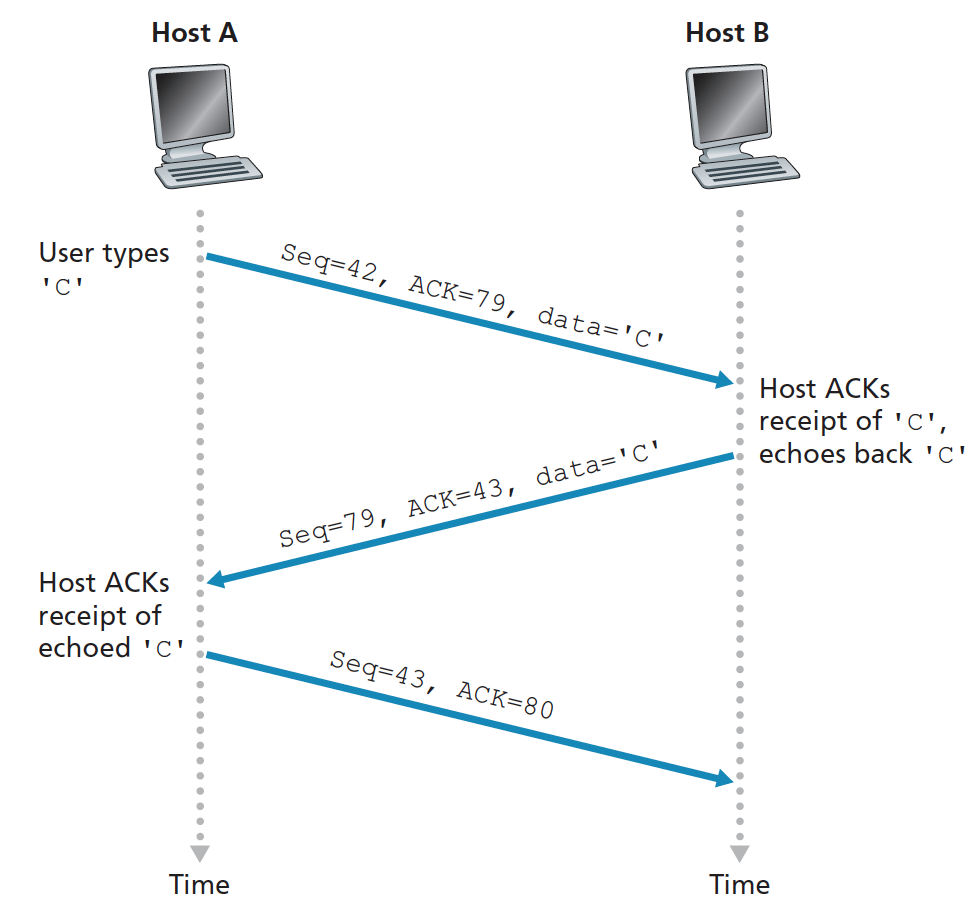
\includegraphics[keepaspectratio, width=15cm, height=12cm]{imagens/12/12 - troca de mensagens tcp.png}
\caption{Sequence number e ACK \\
Imagem retirada de: Computer Networking a top-down approach. 8th
ed.~Pearson, página 234. \\}
\label{Sequence number e ACK}
\end{figure}



\hypertarget{segmentos-fora-de-ordem}{%
\subsubsection{Segmentos fora de ordem}\label{segmentos-fora-de-ordem}}

Como citado anteriormente, o tratamento dos segmentos fora de ordem,
para um sistema confiável de transferência de dados, pode seguir uma
dessas suas estratégias, \emph{GO-BACK-N} ou \emph{Selective Repeat}
(SR). Por uma questão de eficiência, o protocolo SR é a abordagem
praticada.

\hypertarget{rtt-e-timeout}{%
\subsubsection{RTT e Timeout}\label{rtt-e-timeout}}

Depois do envio de um segmento, ao fim de qual intervalo de tempo o TCP
deve considerar que os dados foram perdidos (\texttt{timeout\ interval})
? Esse tempo sofre de uma dicotomia, pois tanto períodos pequenos como
grandes tornam a comunicação ineficiente por causar retransmissões
desnecessárias e aumentar o atraso na retransmissão de segmentos
perdidos, respectivamente.

Podemos considerar que, no mínimo, o tempo esperado deve superar o
\emph{Round-Trip Time} (RTT), período entre o envio de um dado e a
chegada de sua resposta. Como pode-se imaginar, por consequência da não
previsibilidade de uso {[}da rede{]} e da ocorrência de erros, as
condições presentes na rede são variáveis (como um possível
congestionamento), algo que impacta diretamente no (RTT), tornando-o,
também, variável.

Assim, a determinação do \texttt{timeout\ interval} passa por um cálculo
estatístico, definido pelo \texttt{SampleRTT}, uma amostra desse período
medida de tempos em tempos, \texttt{EstimatedRTT}, uma estimativa do
valor do RTT que utiliza a técnica da média móvel exponencialmente
ponderada (EWMA, \emph{Exponential Weighted Moving Average}), e
\texttt{DevRTT}, uma estimativa de quanto o \texttt{SampleRTT} desvia do
\texttt{EstimatedRTT}. Os cálculos podem ser vistos a seguir.

Valores recomendados {[}RFC 6298{]}: α = 0.125 (1/8) β = 0.25 (1/4)

\begin{verbatim}
EstimatedRTT = (1 – α) * EstimatedRTT + α * SampleRTT
\end{verbatim}

\begin{verbatim}
DevRTT = (1 – β) * DevRTT + β * | SampleRTT – EstimatedRTT |
\end{verbatim}

Para questões de eficiência, é interessante manter o valor do
\emph{timeout interval} algo como o valor estimado do RTT
(\texttt{EstimatedRTT}) mais uma margem que se adéque à flutuação de
valor do \texttt{SampleRTT} (\texttt{DevRTT}). Dessa maneira, chegamos
do cálculo a seguir (sendo 1 segundo o valor inicial):

\begin{verbatim}
TimeoutInterval = EstimatedRTT + 4 * DevRTT
\end{verbatim}

\hypertarget{complementar-5}{%
\section{Complementar}\label{complementar-5}}

\hypertarget{pesquisar-sobre-4}{%
\subsection{Pesquisar Sobre}\label{pesquisar-sobre-4}}

\begin{enumerate}
\def\labelenumi{\arabic{enumi}.}
\tightlist
\item
  Flow Control (Computer Networking a top-down approach. 8th
  ed.~Pearson, página 246)
\item
  TCP Connection Management (Computer Networking a top-down approach.
  8th ed.~Pearson, página 249)
\item
  Congestion Control (Computer Networking a top-down approach. 8th
  ed.~Pearson, página 255)
\item
  TCP Congestion Control (Computer Networking a top-down approach. 8th
  ed.~Pearson, página 263) (TCP Cubic, Fairness)
\item
  Evolution of Transport-Layer Functionality (Computer Networking a
  top-down approach. 8th ed.~Pearson, página 279) (QUIC (\emph{Quick UDP
  Internet Connection}))
\end{enumerate}
%\hypertarget{aula-13}{%
%\chapter{Aula: 13}\label{aula-13}}




\hypertarget{ip-o-protocolo-da-network-layer}{%
\chapter{IP, o protocolo da Network Layer}\label{ip-o-protocolo-da-network-layer}}

O objetivo da \emph{network layer} (camada de rede) é transferir dados
de um \emph{host} emissor para o \emph{host} receptor (como não há
garantias, esse serviço é conhecido como \emph{best-effort service}).
Para tal, é necessário determinar a rota (\emph{route} ou \emph{path})
global que os dados devem pecorrer para alcançar o seu destino, chamado
de \emph{routing}, bem como especificar o caminho local com o
direcionamento dos dados recém chegados no roteador para a sua saída
apropriada, chamado de \emph{fowarding}.

Dessa forma, a \emph{network layer} pode ser decomposta em duas partes,
\emph{control plane} e \emph{data plane}, nas quais estão contidos o
\emph{routing} e o \emph{fowarding}, como mostrado na Figura \ref{Control plane e data plane}.

\begin{figure}[h!]
\centering
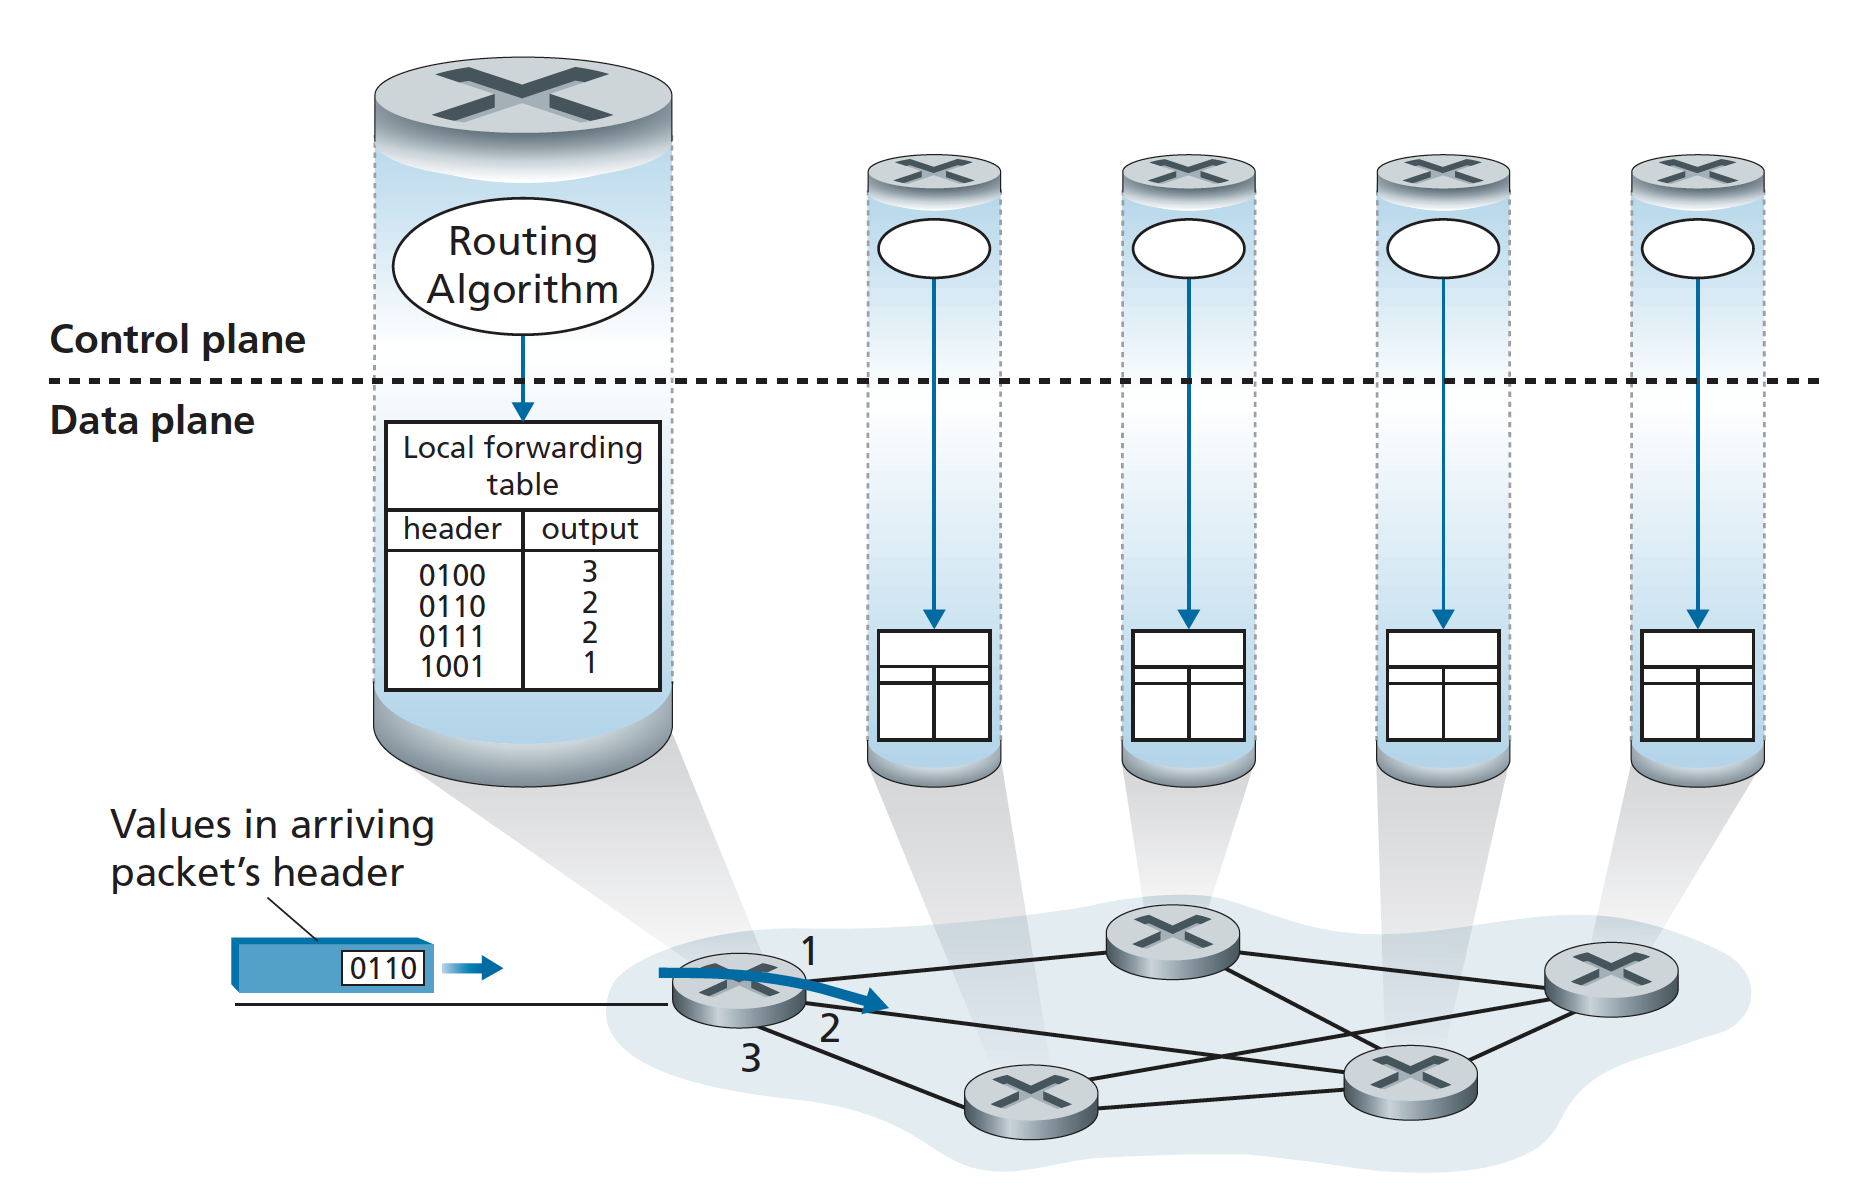
\includegraphics[keepaspectratio, width=15cm, height=12cm]{imagens/13/13 - Control plane and data plane.png}
\caption{Control plane e data plane \\
Imagem retirada de: Computer Networking a top-down approach. 8th
ed.~Pearson, página 307. \\}
\label{Control plane e data plane}
\end{figure}



É importante perceber que apesar dessas duas funcionalidades serem
requisitos para a \emph{network layer}, é possível encontrá-las em
dispositivos separados, algo possibilitado pelo SDN (Software-Defined
Networks), que aloca o \emph{control plane} em um servidor, algo que
torna os roteadores especialistas em \emph{fowarding}.

A \emph{fowarding table}, responsável por determinar, a partir do
\emph{header} dos dados recebidos pelo roteador, a saída apropriada, é o
elemento chave para a interação entre essas partes (\emph{control plane}
e \emph{data plane}), pois seus registros são gerados pelo \emph{control
plane} e utilizados pelo \emph{data plane}.

\hypertarget{protocolo-ip}{%
\section{Protocolo IP}\label{protocolo-ip}}

O IP (\emph{Internet Protocol}) é o protocolo utilizado na camada de
rede. Atualmente está largamente em uso as versões 4 e 6, as quais serão
discutidas a seguir. A estrutura de dados resultante da \emph{network
layer} é o \emph{datagram}, no qual o seu arranjo varia conforme a
versão utilizada.

Citando o livro-texto desse curso:

``Nevertheless, the datagram plays a central role in the internet -
every networking student and professional needs to see it, absorb it,
and master it.'' (Computer Networking a top-down approach. 8th
ed.~Pearson, página 331)

Entender o \emph{datagram} é de suma importância para a aprendizagem de
redes de computadores.

\hypertarget{ipv4-datagram}{%
\section{IPv4 Datagram}\label{ipv4-datagram}}

O \emph{datagram}, como mostrado na Figura \ref{IPv4 Datagra }, segue o seguinte formato:

\begin{enumerate}
\def\labelenumi{\arabic{enumi}.}

\item
  Version Number: especifica a versão utilizada (no caso, 4)
\item
  Header length: a versão 4 do IP tem um tamanho de \emph{header}
  variável, causado pelo campo \emph{options}, o que torna necessário a
  manutenção dessa informação dentro do \emph{datagram} (o campo
  \emph{options} não é normalmente utilizado, portanto o tamanho típico
  do \emph{header} IPv4 \emph{datagram} é de 20 \emph{bytes})
\item
  Type of Service (TOS): exemplos são \emph{real time},
  \emph{non-real-time}.
\item
  Datagram length: o tamanho do \emph{datagram} é calculado pela soma
  dos tamanhos do header dos dados carregados (\emph{payload}). Composto
  por 16 bits e medido em \emph{bytes}, o tamanho teórico máximo é de
  65535 bytes (raramente ultrapassa os 1500 bytes).
\item
  Identifier, flags e fragmentation offset: utilizados para fragmentar
  um \emph{datagram} muito grande em pedaços pequenos que serão enviados
  independentemente e remontados no destino.
\item
  time-to-live (ttl): decrementa em 1 toda vez que o \emph{datagram} é
  processado por um roteador, sendo descartado ao atingir 0.
\item
  Protocol: indica o protocolo da camada de transporte. contém o valor
  de 6 (00110) para TCP e 17 (10001) para UDP.
\item
  Header Checksum: Objetivando detectar erros, esse campo é computado
  tratando cada 2 bytes do \textbf{header} como um número e somando-os
  utilizando a aritmética complementar de 1. Esse cáculo é somente feito
  para o \textbf{header}, evitando possíveis redundâncias com as camadas
  inferiores.
\item
  Source e destination IP addresses.
\item
  Options: permite uma extensão do \emph{header}. Não foi incluido no
  \emph{datagram} do IPv6 por dificultar a determinação do início do
  \emph{payload} (necessitando do campo \emph{header length}) e a
  variação do tempo requerido para processamento (pois alguns
  \emph{datagrams} podem requisitar ou não o processamento do campo
  \emph{options}).
\item
  Data (payload): contém o segmento da camada de transporte.
\end{enumerate}



\begin{figure}[h!]
\centering
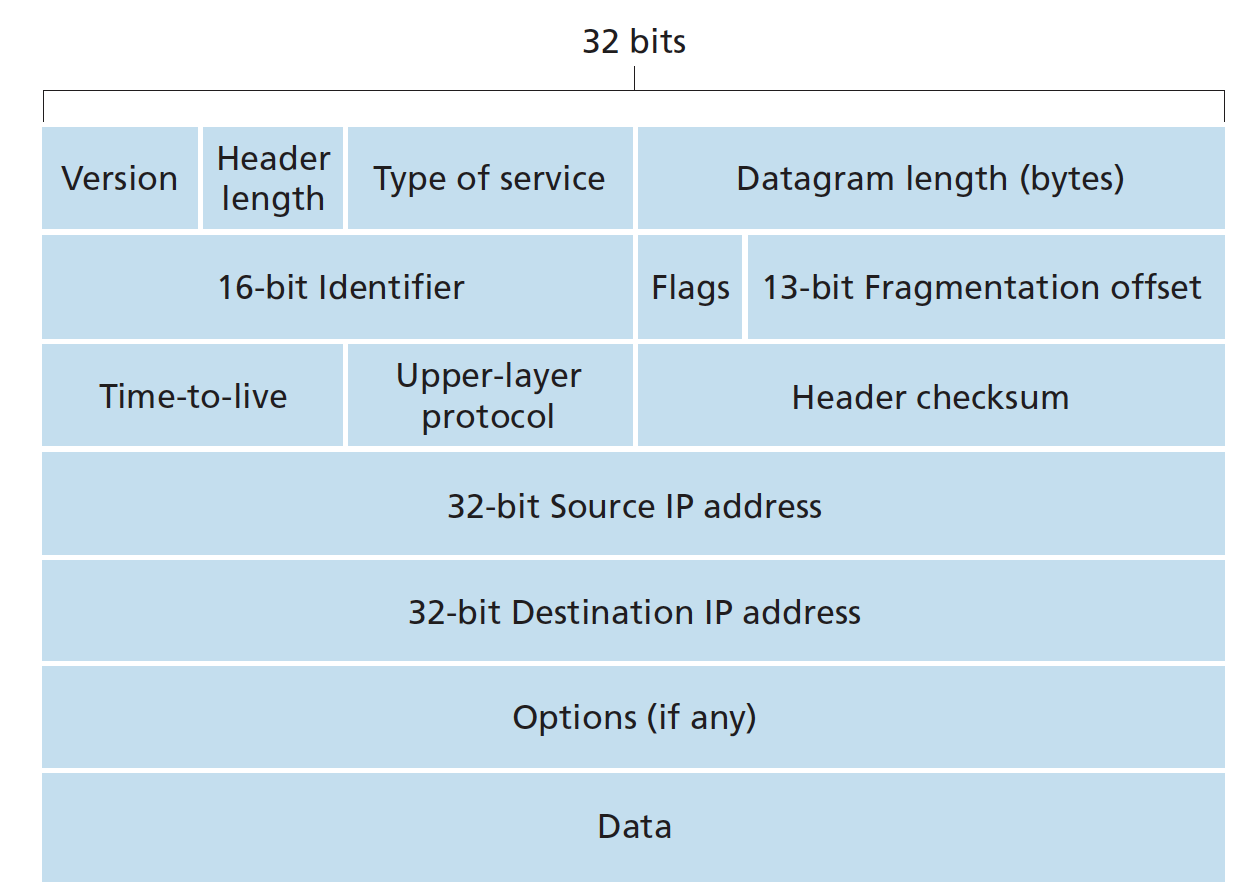
\includegraphics[keepaspectratio, width=12cm, height=9cm]{imagens/13/13 - IPv4 Datagram.png}
\caption{IPv4 Datagra \\
Imagem retirada de: Computer Networking a top-down approach. 8th
ed.~Pearson, página 331. \\}
\label{IPv4 Datagra }
\end{figure}





\hypertarget{endereuxe7amento}{%
\section{Endereçamento}\label{endereuxe7amento}}

A fronteira entre o \emph{host} e a conexão física é chamada de
interface. Em um roteador é possível identificar multiplas interfaces.
Como cada interface está associado um endereço de IP, um roteador,
portanto, pode estar associado a múltiplos endereços de IP. O endereço
de IP é formado por 4 bytes (32 bits), escritos na notação
\emph{dotted-decimal}, no qual cada byte é escrito em decimal e separado
por um ponto.

O endereçamento segue a estratégia conhecida como \emph{Classless
Interdomain Routing} (CIDR), no qual o endereço de IP (formado por 32
bits) é separado em prefixo (os \texttt{x} primeiros bits) e
identificador de host (os restantes \texttt{32\ -\ x} bits). O número de
bits (\texttt{x}) que formam o prefixo é determinado pela máscara de
rede (\emph{mask subnet}), como mostrado a seguir:

\begin{verbatim}
Endereço de IP: a.b.c.d
Endereço de IP com máscara de rede: a.b.c.d/x
Notação: 193.32.216.9/24 (11000001 00100000 11011000 00001001)
Prefixo (Sub-rede): 193.32.216 (11000001 00100000 11011000)
Identificador de Host: 9 (00001001)
\end{verbatim}

A máscara de sub-rede (\emph{network mask}) distingue o endereço
referente à sub-rede ao do \emph{host}. A sub-rede pode ser entendida como
uma ilha de rede isolada, com as interfaces compondo as bordas dessa
rede, como mostrado na Figura \ref{Subrede}.


\begin{figure}[h!]
\centering
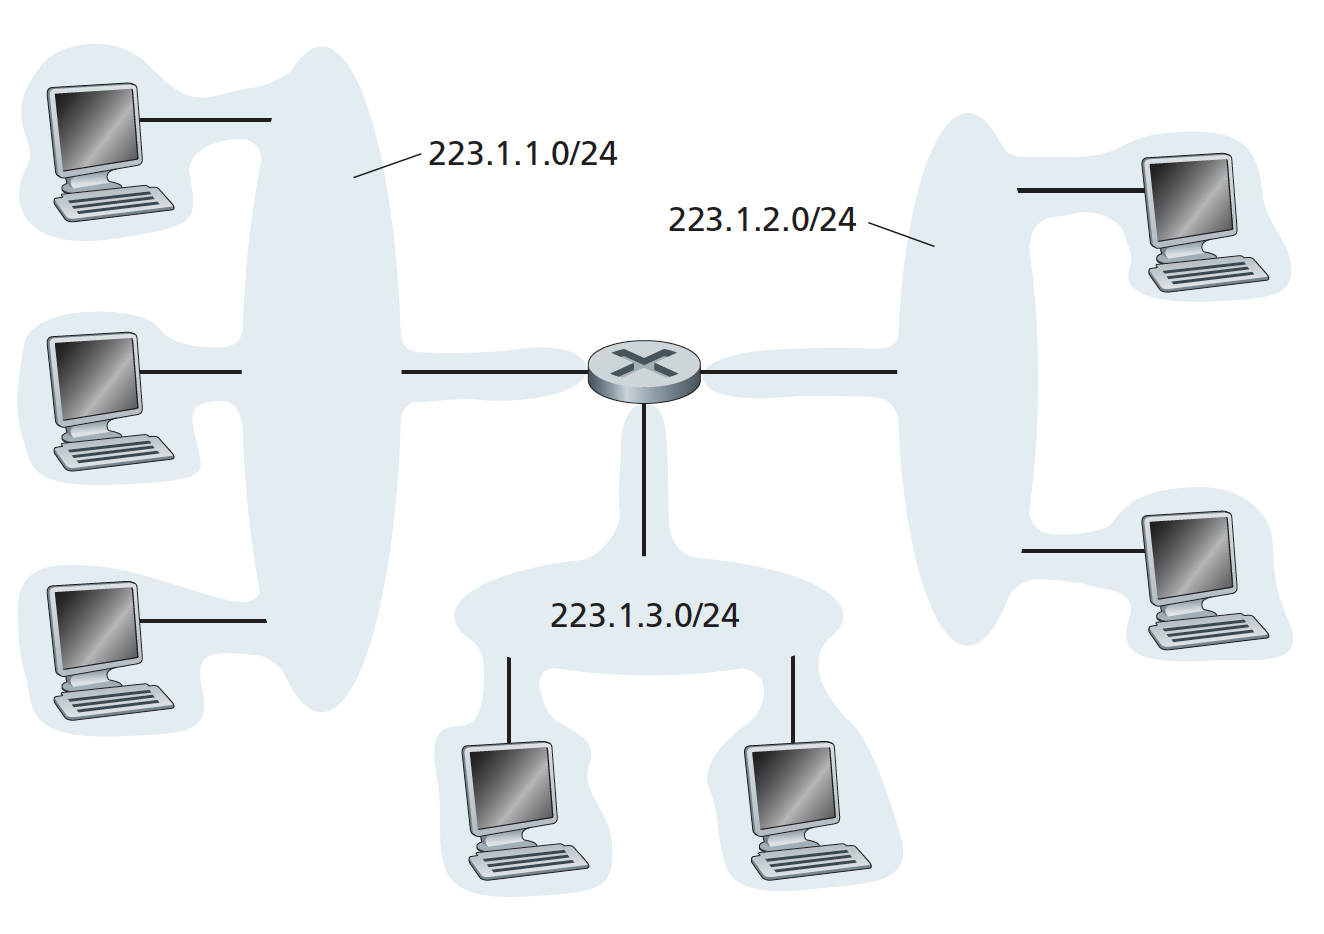
\includegraphics[keepaspectratio, width=12cm, height=9cm]{imagens/13/13 - subnet.png}
\caption{Sub-rede \\
Imagem retirada de: Computer Networking a top-down approach. 8th
ed.~Pearson, página 336. \\}
\label{Subrede}
\end{figure}





\hypertarget{obter-um-endereuxe7o-de-ip}{%
\subparagraph{Obter um endereço de
IP}\label{obter-um-endereuxe7o-de-ip}}

A obtenção de um endereço de IP ocorre de forma automática com o
protocolo DHCP (\emph{Dynamic Host Configuration Protocol}), chamado
também de protocolo \emph{plug-and-play} ou \emph{zeroconf} (\emph{zero
configuration}), o qual gera um endereço de IP temporário diferente toda
vez que o \emph{host} conecta-se nessa rede. O DHCP é um protocolo
baseado na arquitetura \emph{client-server}, e o seu processo é feito em
quatro passos (mostrado na Figura \ref{Processo DHCP }):

\begin{enumerate}
\def\labelenumi{\arabic{enumi}.}
\tightlist
\item
  Server Discovery: o \emph{client} dispara \emph{datagram} contendo um
  \emph{discovery message} para o destino 255.255.255.255 (esse endereço
  de IP indica ao roteador que a mensagem deva ser entregue para todos
  as interfaces da sub-rede), com a origem em 0.0.0.0.
\item
  Server Offer: O Servidor DHCP, após receber a discovery message\emph{,
  responde com a }offer message* para 255.255.255.255 (ou seja,
  disparando para todos os dispositivos da subrede). A \emph{offer
  message} contém: uma proposta de \emph{IP address}; \emph{network
  mask}; e o \emph{IP address lease time}, referente à validade do IP. É
  importante perceber que na mesma rede pode haver múltiplos servidores
  DHCP e, portanto, múltiplas \emph{offer message} podem ser disparadas
  durante essa etapa.
\item
  Request: o \emph{client} escolhe uma \emph{server offer} e ecoa os
  seus parâmetros com a \emph{request message}.
\item
  ACK: o servidor selecionado confirma a seleção do endereço enviando
  uma \emph{ACK message}.
\end{enumerate}


\begin{figure}[h!]
\centering
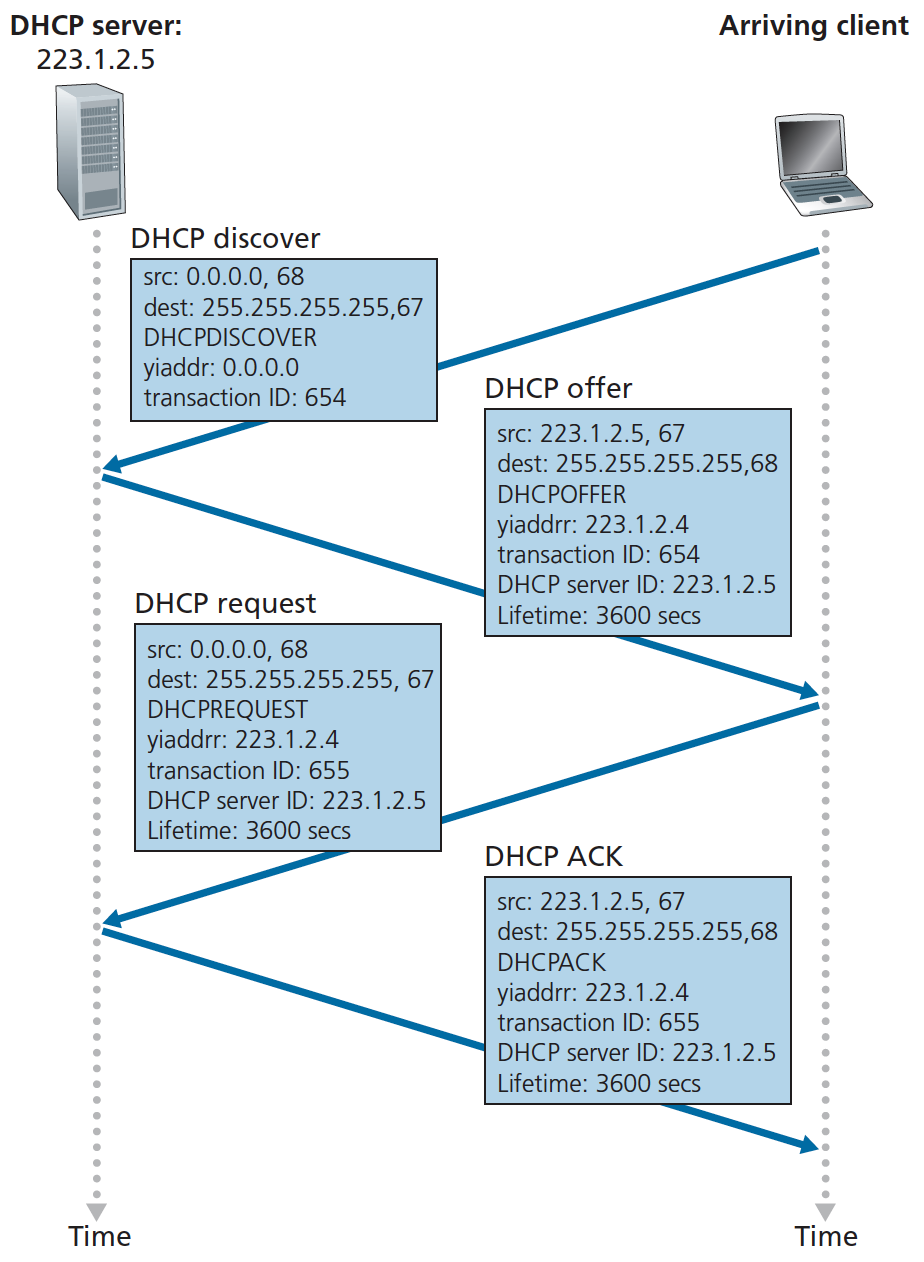
\includegraphics[keepaspectratio, width=18cm, height=15cm]{imagens/13/13 - DHCP process.png}
\caption{Processo DHCP \\
Imagem retirada de: Computer Networking a top-down approach. 8th
ed.~Pearson, página 343. \\}
\label{Processo DHCP }
\end{figure}


\hypertarget{nat}{%
\section{NAT}\label{nat}}

\begin{enumerate}
\def\labelenumi{\arabic{enumi}.}
\tightlist
\item
  Como um servidor DHCP local geraria um IP único diferente de um outro
  servidor geograficamente distante ?
\item
  Os diferentes servidores DHCP devem estar sincronizados ou faixas
  específicas de IP devem ser pré-determinadas ?
\item
  Eu já encontrei redes domésticas com a mesma faixa de endereço de IP,
  como isso é possível ?
\end{enumerate}

Essas e outras perguntas vem à tona quando é imaginado como funcionaria
uma interação global de sub-redes. A solução passa pelo uso do protocolo
NAT (\emph{Network Address Translation}), mostrado na Figura \ref{NAT}.



\begin{figure}[h!]
\centering
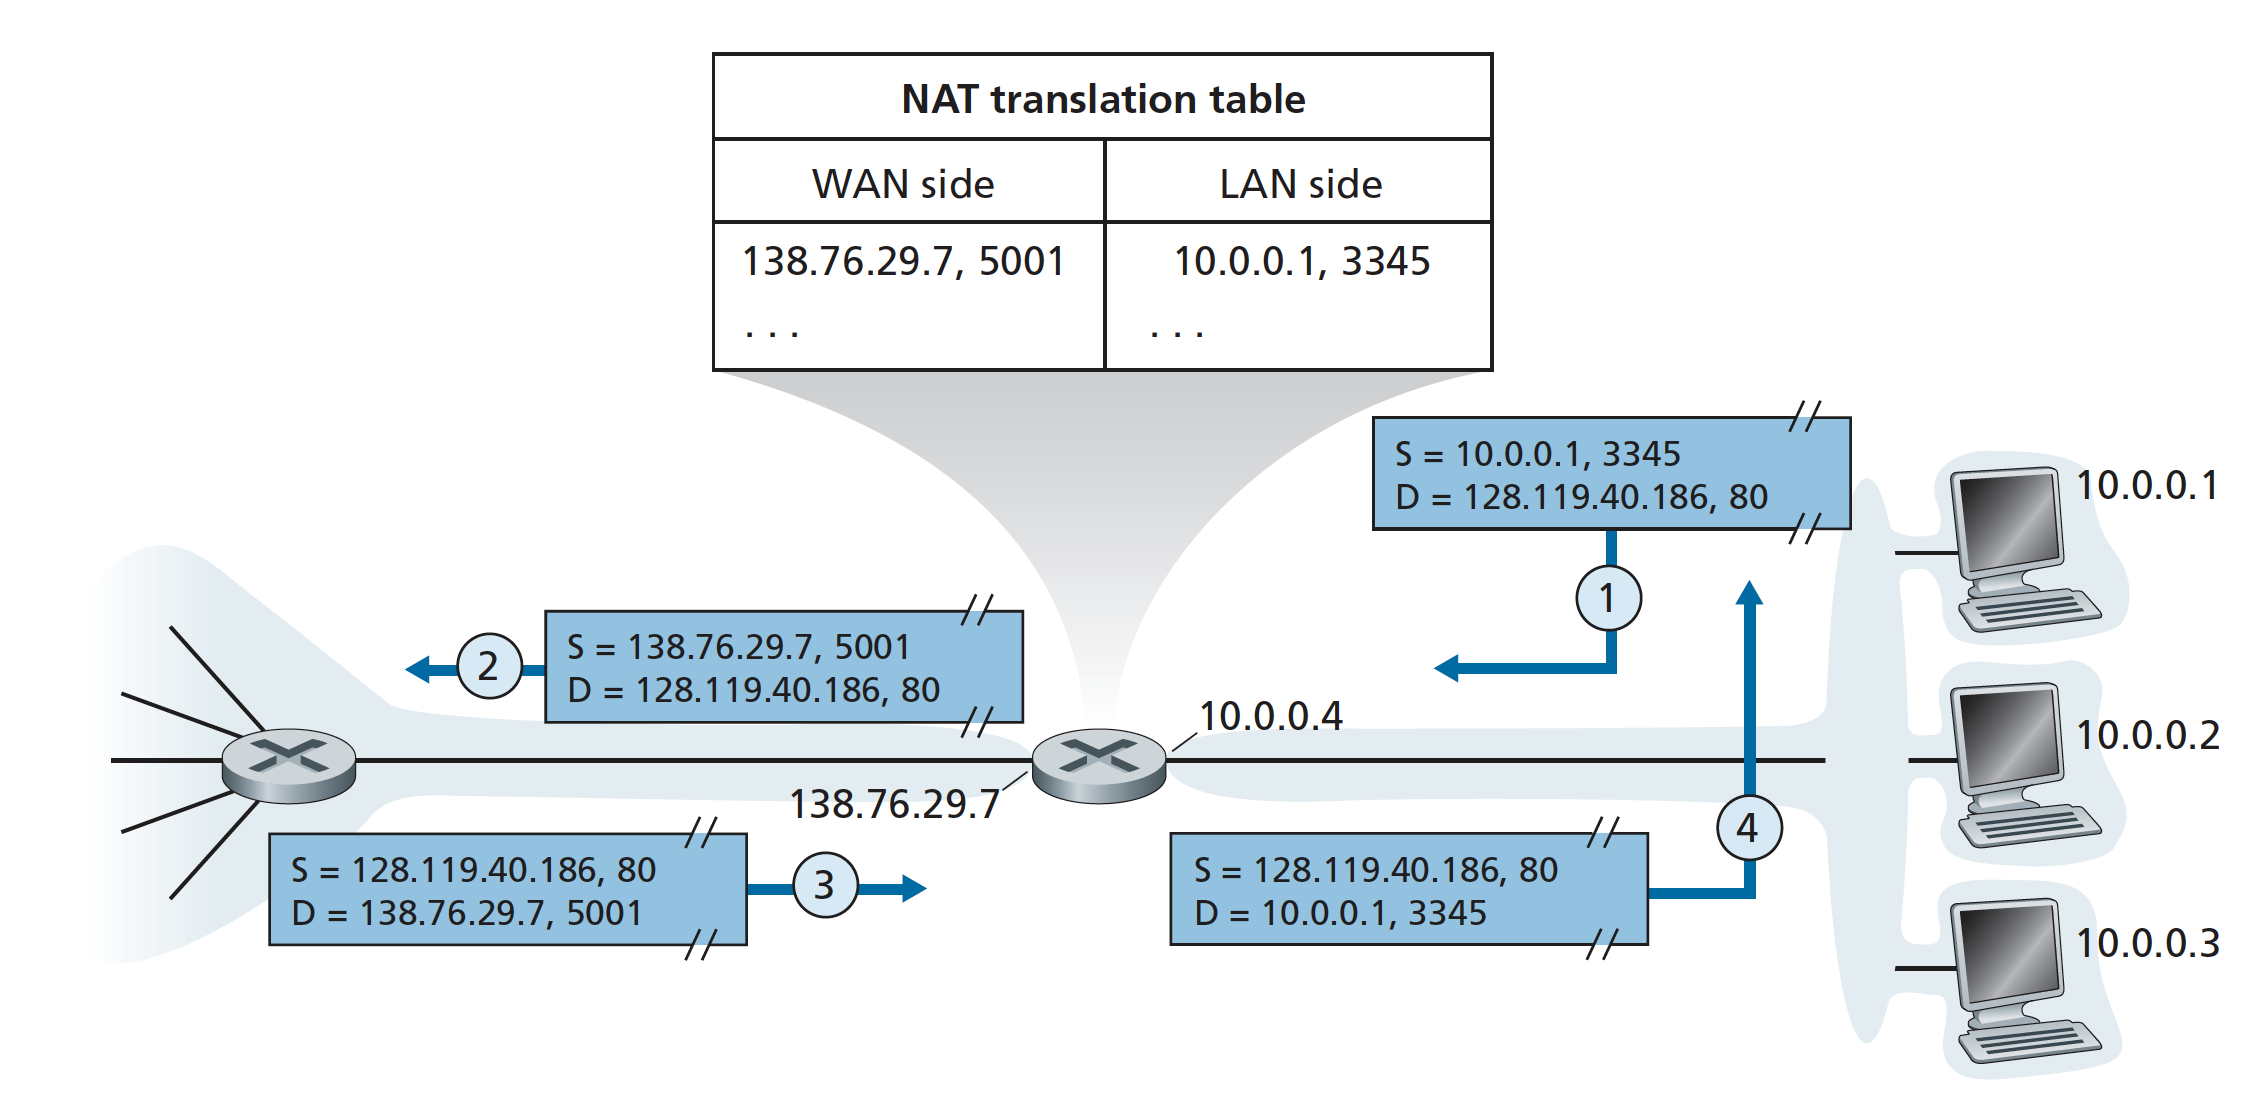
\includegraphics[keepaspectratio, width=15cm, height=12cm]{imagens/13/13 - NAT.png}
\caption{NAT \\
Imagem retirada de: Computer Networking a top-down approach. 8th
ed.~Pearson, página 345. \\}
\label{NAT}
\end{figure}





Um roteador com o protocolo NAT ativo é visto como um dispositivo único
(com o IP único) para o resto do mundo, escondendo, assim, os detalhes
das configurações de uma rede doméstica para as redes externas.

É interessante notar que o roteador obtém o endereço de IP via o
servidor DHCP oriundo do ISP (\emph{Internet Service Provider}). E por
sua vez, oferece um servidor DHCP para a sua sub-rede.

O segredo para o funcionamento do NAT está no \emph{NAT translation
table}.

Quando uma requisição é disparada por um \emph{host} para um
\emph{server} fora da rede, o roteador converte o endereço de IP de
origem para o seu, e gera uma nova porta. Dessa forma, a \emph{NAT
translation table} é populada, no lado WAN (rede do ISP), com endereço
de IP do roteador e porta gerada, e no lado LAN (rede doméstica),
endereço de IP do \emph{host} e porta da \emph{Thread}.

Por exemplo:

\begin{enumerate}
\def\labelenumi{\arabic{enumi}.}
\tightlist
\item
  \emph{Host} dispara um \emph{datagram} com origem 10.0.0.1 e porta
  3345 para o \emph{server} 128.119.40.186 porta 80.
\item
  O roteador gera uma nova porta e substitui os parâmetros de origem
  para essa porta gerada e para o seu endereço de IP (que por sua vez
  foi gerado pelo ISP). E registra essa conversão no \emph{NAT
  translation table}.
\item
  O \emph{server} recebe o \emph{datagram} com os parâmetros de origem
  do roteador, e o responde.
\item
  O roteador converte os parâmetros de destino utilizando a tabela NAT,
  e, por fim, direciona o \emph{datagram} recebido ao \emph{host}.
\end{enumerate}

Esse registro é mantido até o fim da conexão. Como o tamanho do campo
porta é de 16 bits, o protocolo NAT suporta mais de 60 mil conexões com
somente um único \emph{IP address}.

Um dos problemas causados por esses protocolos (DHCP e NAT) é referente
aos \emph{Home Servers}, pois como um servidor espera por uma requisição
de um \emph{client}, como esse \emph{client} pode saber qual é o atual
endereço de IP do servidor ? Como funcionaria a arquitetura P2P ?
Soluções para esse problema incluem \emph{NAT transversal tools} {[}RFC
5389, RFC 5128{]}, algo que não será debatido nesse texto.

\hypertarget{ipv6-datagram}{%
\section{IPv6 datagram}\label{ipv6-datagram}}

Há uma série de mudanças introduzidas com o IPv6, mostrado na Figura \ref{IPV6 Datagram}:


\begin{figure}[h!]
\centering
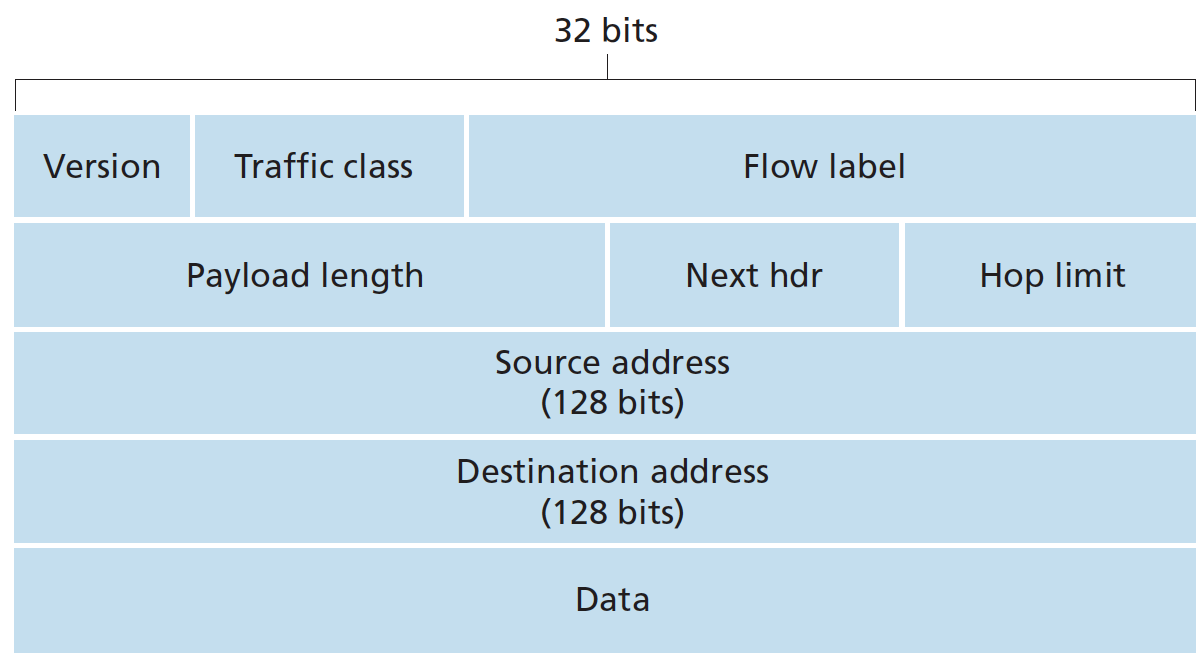
\includegraphics[keepaspectratio, width=12cm, height=9cm]{imagens/13/13 - IPv6 datagram.png}
\caption{IPV6 Datagram \\
Imagem retirada de: Computer Networking a top-down approach. 8th
ed.~Pearson, página 349. \\}
\label{IPV6 Datagram}
\end{figure}


\begin{enumerate}
\def\labelenumi{\arabic{enumi}.}
\tightlist
\item
  Capacidade de endereçamento expandido: de 32 bits para 128 bits
\item
  \emph{header} de tamanho fixo: o \emph{header} foi fixado em 40
  \emph{bytes}, permitindo um processamento mais rápido pelo roteador
\item
  fluxo e seu rótulo: capacidade de rotular os \emph{datagrams} de um
  fluxo específico, o qual cada rótulo sinaliza uma requisição
  específica, como \emph{real-time service} ou \emph{non-default
  quality}
\end{enumerate}

Os campos do \emph{datagram} do IPv6 são:

\begin{enumerate}
\def\labelenumi{\arabic{enumi}.}
\tightlist
\item
  Version: versão do IP (no caso, 6).
\item
  Traffic class: equivalente ao TOS do IPv4, é usado para dar prioridade
  à algum \emph{datagram}
\item
  \emph{flow label}: campo de 20 \emph{bits} usado para rotular um fluxo
  de \emph{datagrams}
\item
  \emph{Payload Length}: campo de 16 \emph{bits} que indica o tamanho do
  \emph{payload}
\item
  \emph{Next Header}: identifica o protocolo para qual o \emph{datagram}
  (ou o \emph{payload}) será entregue
\item
  \emph{Hop limit}: equivalente ao TTL do IPv4, diminui em 1 toda vez
  que o \emph{datagram} é transmitido por um roteador e descartado
  quando chega em 0.
\item
  Endereço de origem e destino: no formato de 128 \emph{bits}
\item
  \emph{Data}: também chamado de \emph{payload}, é o conteúdo
  encapsulado pelo protocolo.
\end{enumerate}

Foram removidos:

\begin{enumerate}
\def\labelenumi{\arabic{enumi}.}
\tightlist
\item
  Fragmentação e remontagem: IPv6 não permite a fragmentação e a
  remontagem do datagram (essa operação era feita com o objetivo de
  reduzir o tamanho do \emph{datagram} grande demais para ser
  transmitido). Assim caso um \emph{datagram} seja muito grande, o
  roteador descarta esse \emph{datagram} e retorna uma mensagem de erro,
  de forma que o emissor deverá reenviar o \emph{datagram}. A remoção
  dessa funcionalidade gera, como resultado, uma redução no tempo de
  processamento do roteador.
\item
  \emph{Header checksum}: Considerado suficientemente redundante e
  enfatizando a velocidade de processamento, esse campo não se mostrou
  necessário para os desenvolvedores do IPv6.
\item
  Options: a remoção do \emph{options} possibilitou a fixação do tamanho
  do \emph{header} em 40 \emph{byts}, algo que além de causar um
  encolhimento no tempo de processamento, também deixa explícito o
  início do \emph{payload} (afinal, o \emph{payload} sempre estará 40
  bytes após o início do \emph{datagram}).
\end{enumerate}

\hypertarget{transiuxe7uxe3o-de-ipv4-para-ipv6}{%
\section{Transição de IPv4 para IPv6}\label{transiuxe7uxe3o-de-ipv4-para-ipv6}}

Há um problema inerente na atualização dos sistemas distribuídos: a
adoção de uma nova tecnologia por todos os elementos da rede Um sistema
com o IPv6 pode ser projeto para ser retro-compatível com o IPv4, mas um
sistema com IPv4 não é capaz de lidar com o IPv6.

Como, então, atualizar todos os incontáveis dispositivos já integrados
na rede ?

\begin{enumerate}
\def\labelenumi{\arabic{enumi}.}
\tightlist
\item
  Transição abrupta: substituir todos os elementos de uma vez só,
  marcando um dia x para inutilizar os dispositivos compatíveis com
  IPv4.
\item
  Transição suave: substituir os elementos de forma gradual.
\end{enumerate}

A abordagem da transição suave foi o caminho escolhido. Para tal, fora
adotado a prática do \emph{tunneling} (algo que torna os dispositivos
IPv6 compatível com o IPv4). O \emph{tunnel} encapsula o \emph{datagram}
do IPv6 integralmente, tornando-o o \emph{payload} do IPv4, resultando
em um \emph{datagram} com o \emph{header} do IPv4 (como mostrado na Figura \ref{Tunneling}).


\begin{figure}[h!]
\centering
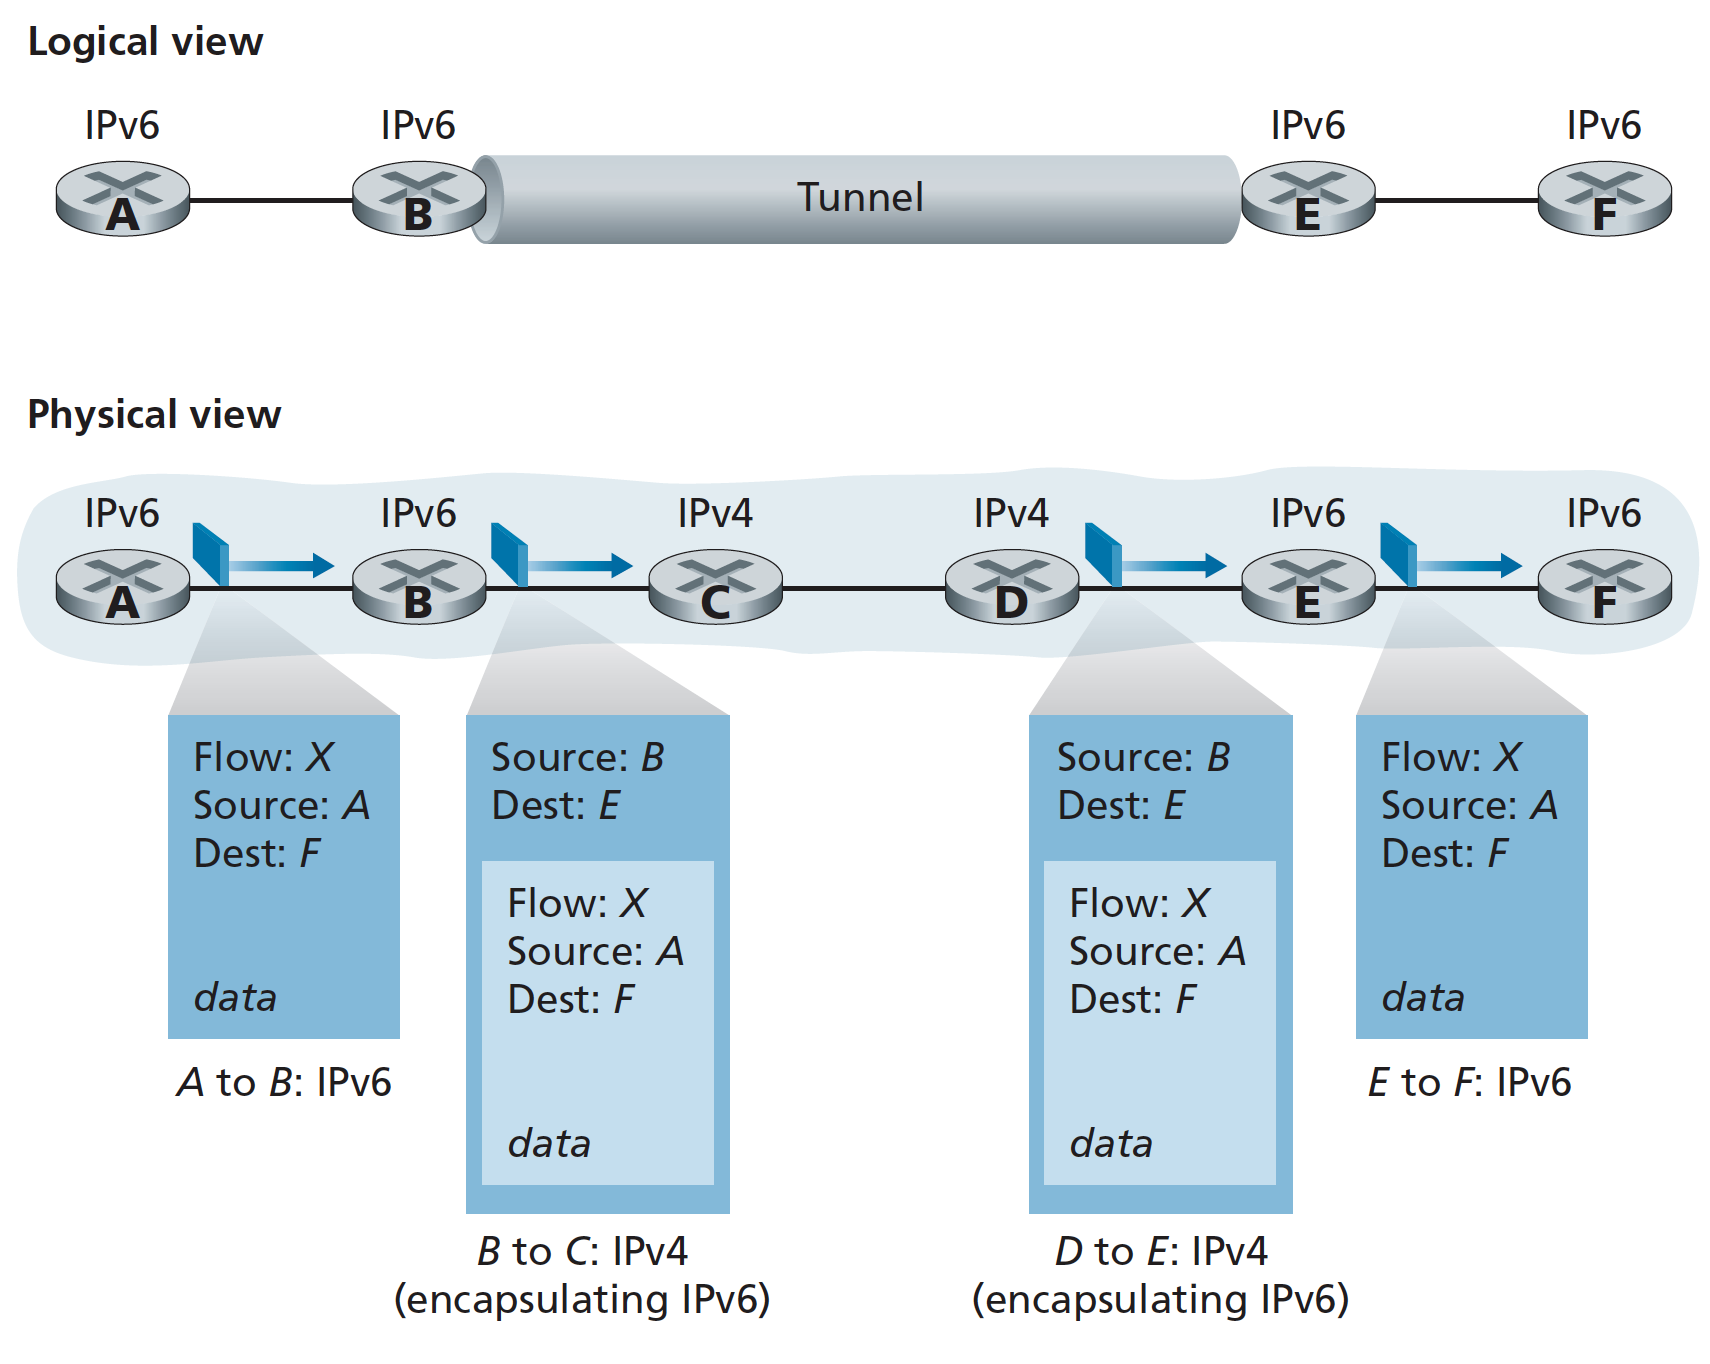
\includegraphics[keepaspectratio, width=14cm, height=11cm]{imagens/13/13 - Tunneling.png}
\caption{Tunneling \\
Imagem retirada de: Computer Networking a top-down approach. 8th
ed.~Pearson, página 352. \\}
\label{Tunneling}
\end{figure}



\hypertarget{link-layer}{%
\chapter{Link Layer}\label{link-layer}}

Após a \emph{Network Layer} determinar qual o caminho de comunicação
(chamado de \emph{link} ou enlace) o \emph{datagram} deve percorrer, como
o \emph{WiFi} ou o \emph{Ethernet}, entra em cena o \emph{Link Layer}
(camada de enlace), responsável por encapsular o \emph{datagram} e
transmitir o resultado (o \emph{frame}) através do \emph{link}. Os
dispositivos que executam a camada de enlace são chamados de nós
(\emph{nodes}).

Fundamentalmente, os \emph{links} podem ser classificados em dois canais
de comunicação. O primeiro refere-se aquele no qual os nós compartilham
do mesmo caminho de transmissão (\emph{single broadcast link}), como os
\emph{wireless LANs}. O segundo tipo é de ponto-a-ponto, no qual somente
dois nós são conectados em cada \emph{link}.

O \emph{link layer} está presente tanto em \emph{software} (com, por
exemplo, a montagem das informações de endereçamento e o controle de
interrupções) como em \emph{hardware} (com, por exemplo, \emph{link
access} e \emph{framing}) e é implementado em um \emph{chip} chamado de
\emph{Network Interface Controller} (NIC).

\hypertarget{serviuxe7os}{%
\section{Serviços}\label{serviuxe7os}}

A camada de enlace provê os seguintes serviços:


\begin{enumerate}
\def\labelenumi{\arabic{enumi}.}
\tightlist
\item
  \emph{Framing}: constituição do \emph{frame} a partir do
  encapsulamento do \emph{datagram}.
\item
  \emph{Link access}: o controle de acesso é algo fundamental para a
  realização da transmissão, sendo esse realizado pelo \emph{Medium
  Access Protocol} (MAC protocol). Nos \emph{links} ponto-a-ponto, o
  protocolo somente verifica se o \emph{link} está disponível. Em
  \emph{single broadcast link}, ocorre o problema de multiplos acessos
  simultâneos, sendo da responsabilidade do protocolo MAC especificar as
  regras para a transmissão dos \emph{frames}
\item
  \emph{Reliable delivery}: protocolo que objetiva garantir a transmissão
  de cada \emph{datagram}.
\item
  \emph{Error detection and corretion}: devido à possíveis erros
  introduzidos pela atenuação do sinal ou ruídos eletromagnéticos,
  vários protocolos fornecem mecanismos de detecção e correção de erros.
\end{enumerate}

\hypertarget{endereuxe7amento-o-switches}{%
\section{Endereçamento}\label{endereuxe7amento-o-switches}}

O \emph{Link Layer} utiliza um sistema de endereçamento similar ao
\emph{Network Layer} com o \emph{IP Address}.

Na fabricação de um NIC, lhe é designado um endereço único de 6 bytes
chamados de \emph{MAC Address} (\emph{LAN Address}, ou \emph{Physical
Address}), que se complementa ao \emph{IP Address} de forma similar à
relação entre o CPF de um brasileiro com seu endereço residencial, pois
o endereço residencial é alterado conforme ocorre uma mudança (assim
como o \emph{IP Address} é alterado após o dispositivo mudar de rede),
mas o seu CPF não é modificado (assim como o \emph{MAC Address}).
Portanto, é designado (pelo fabricante) ao NIC um \emph{MAC Address}, e
(pela rede) um \emph{IP Address}.

\hypertarget{arp}{%
\subsection{ARP}\label{arp}}

O \emph{Link Layer} necessita, para o envio de seus \emph{frames}, o
endereço MAC do dispositivo receptor. Mas como obter esse endereço ?
Esse endereço pode ser obtido através do \emph{Address Resolution
Protocol} (ARP), no qual armazena em uma tabela (ARP \emph{table}) as
equivalências entre \emph{IP Address} e \emph{MAC Address}. A ARP
\emph{table} está localizada nos NICs de cada \emph{host} e
\emph{router} da sub-rede.

O ARP é similar ao DNS, com a diferença de estar limitado à sua sub-rede
(diferente do DNS que está disponível para toda a Internet).

\hypertarget{funcionamento-do-arp}{%
\subsubsection{Funcionamento do ARP}\label{funcionamento-do-arp}}

Suponha que o \emph{host} 222.222.222.220 quer enviar um \emph{datagram}
para 222.222.222.222, mas não tenha em sua ARP \emph{table} o registro
contendo a equivalência entre o IP e o MAC \emph{Address}. Para tal, o
emissor deve utilizar o protocolo ARP:

\begin{enumerate}
\def\labelenumi{\arabic{enumi}.}
\tightlist
\item
  O emissor deve inquerir (\emph{query}) todos os \emph{hosts} e
  \emph{routers} da sub-rede para determinar a equivalência. Esse
  inquérito ocorre com a montagem de um ARP \emph{packet} (uma estrutura
  especial que contém o endereço IP e MAC do emissor e do receptor)
  destinado ao \emph{MAC Broadcast Address} (um endereço específico,
  FF-FF-FF-FF-FF-FF, no qual sinaliza que a transmissão deve ser feito
  para todos os \emph{hosts} da sub-rede)
\item
  O NIC encapsula o ARP \emph{packet} em um \emph{link layer frame} e
  transmite para a sub-rede (equivalente a uma pessoa gritar em uma sala
  quem tem um CPF XXX.XXX.XXX-XX)
\item
  O \emph{host} no qual o seu módulo ARP contém o registro inquerido
  envia de volta (diretamente ao inquisidor) um \emph{response} ARP
  \emph{packet} com o mapeamento desejado.
\item
  O \emph{host} inquisidor, por fim, pode atualizar sua ARP \emph{table}
  e enviar os seus dados para o endereço MAC correspondente à
  inquisição.
\end{enumerate}

É importante perceber que: 1. O \emph{query} ARP \emph{message} é
enviado para todos em \emph{broadcast}, enquanto que sua resposta não
(ela é enviada em um \emph{frame} padrão). 2. ARP é
\emph{plug-and-play}, montando sua tabela automaticamente. 3. O ARP é um
protocolo localizado entre o \emph{Network Layer} e o \emph{Link Layer},
por conter parâmetros oriundos de ambas as camadas (como o \emph{IP
Address} e o MAC \emph{Address}, respectivamente) 4. O ARP opera quando
um \emph{host} quer enviar um \emph{datagram} para outro \emph{host} na
mesma sub-rede.

Como um emissor pode enviar um \emph{datagram} para fora de sua rede se
o MAC \emph{Address} de destino é necessário e o protocolo ARP não
fornece o endereço de dispositivos fora da sub-rede ?

A resposta: Não é necessário que o emissor saiba do MAC \emph{Address} do
\emph{host} de destino ! Basta o emissor popular o campo MAC
\emph{Address} de destino com o MAC \emph{Address} do roteador da sua
rede! (Que pode ser obtido pelo ARP)

O roteador da rede do emissor receberá o \emph{datagram} e avaliará para
qual NIC esse \emph{datagram} deve ser direcionado (isso é feito
consultando o \emph{fowarding table}). Uma vez no NIC (da sub-rede 2), o
módulo ARP é acionado para obter o MAC \emph{Address} do destinatário.
Por fim, o \emph{datagram} é encapsulado pelo \emph{Link Layer} e
transmitido para o receptor da mensagem.

\hypertarget{ethernet}{%
\section{Ethernet}\label{ethernet}}

O protocolo \emph{Ethernet} foi inventado nos anos 1970 por Bob Metcalfe
e David Boggs. Inicialmente utilizava um barramento coaxial (uma
\emph{broadcast} LAN) para interconectar os nós. Os padrões utilizados
eram os 10BASE-2 e 10BASE-5 (10 refere-se à velocidade, em Mbps, BASE ao
\emph{baseband} Ethernet, significando que a mídia física só carrega o
tráfico de dados Ethernet, e a parte final refere-se a mídia física em
si, como o cabo coaxial), os quais especificavam 10Mbps Ethernet em
cabos coaxiais limitados a 500 metros. Distâncias maiores poderiam ser
obtidas com o uso dos \emph{repeaters}, dispositivos da camada física
que repetem o sinal de entrada na sua saída.

Em 1990, os barramentos coaxiais foram substituídos pelo cabo de cobre
de par trançado conectado em um Hub, um dispositivo da camada física
(\emph{1-layer}) que retransmite os bits de entrada para todos os nós
conectados a ele, em uma arquitetura estrela (com todos os \emph{hosts}
conectados ao dispositivo central, o Hub), mantendo-se, portanto, uma
\emph{broadcast} LAN. Um problema presente nos \emph{Hubs} ocorre quando
múltiplos \emph{frames} são transmitidos simultaneamente, algo que gera
uma colisão, e os nós que criaram os \emph{frames} devem
retransmiti-los.

A solução para as colisões veio nos anos 2000, quando o \emph{Hub} fora
substituído pelo \emph{Switch}, dispositivo de segunda camada
(\emph{2-layer}, camada de enlace) que armazenam e transmitem
(\emph{store-and-foward}) os dados utilizando o \emph{MAC Address} para
direcioná-los aos seus respectivos \emph{links}, tornando, assim,
dispensável o uso do protocolo MAC (protocolo para controle de colisão).

O \emph{Ethernet} tornou-se o protocolo dominante em redes LAN
(\emph{Local Area Network}) por:

\begin{enumerate}
\def\labelenumi{\arabic{enumi}.}
\tightlist
\item
  Ser o primeiro a implantar largamente o \emph{high-speed} LAN
\item
  Era mais simples e barato do que seus concorrentes
\item
  \emph{Data rates} compatíveis ou maiores do que os seus concorrentes
\item
  Por consequência de sua popularidade, dispositivos \emph{Ethernet} são
  mais baratos.
\end{enumerate}

É importante perceber que, apesar da intensa mudança de padrão sofrida
desde os anos 1970, o Ethernet ainda utiliza a mesma estrutura de
\emph{frame}, algo que será debatido posteriormente.

\hypertarget{ethernet-frame}{%
\subsection{Ethernet Frame}\label{ethernet-frame}}

O \emph{frame} do Ethernet, como mostrado na Figura \ref{Estrutura do frame Ethernet}, é composto por:


\begin{figure}[h!]
\centering
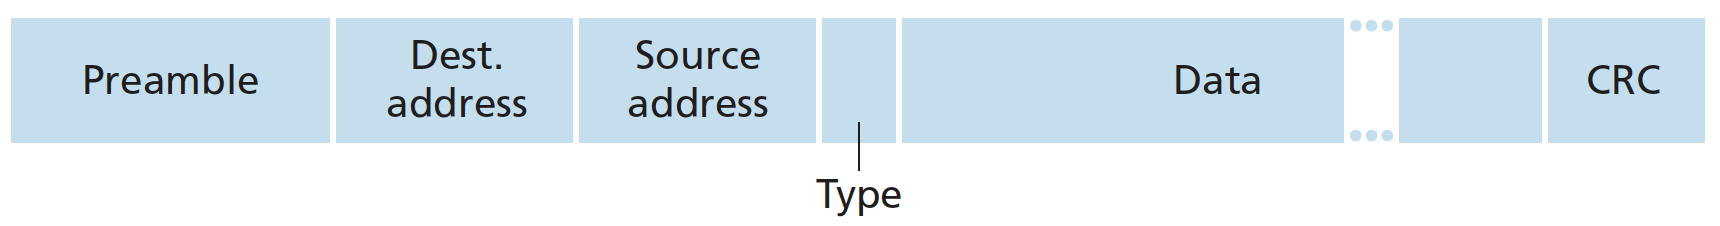
\includegraphics[keepaspectratio, width=12cm, height=9cm]{imagens/13/13 - estrutura do frame ethernet.png}
\caption{Estrutura do frame Ethernet \\
Imagem retirada de: Computer Networking a top-down approach. 8th
ed.~Pearson, página 486. \\}
\label{Estrutura do frame Ethernet}
\end{figure}


\begin{enumerate}
\def\labelenumi{\arabic{enumi}.}
\tightlist
\item
  \emph{Data Field} (\emph{payload}): é o local no qual é carregado o
  \emph{datagram} (resultado da camada superior). Tem o tamanho máximo
  (\emph{Maximum Transmission Unit}, MTU) de 1500 \emph{bytes} e mínimo
  de 46 \emph{bytes}. Caso o \emph{datagram} seja maior, o \emph{host}
  deve fragmentá-lo. Caso seja menor, o campo \emph{Data Field} é
  preenchido (\emph{stuffed}) até o mínimo (o campo \emph{length}
  presente no \emph{header} do \emph{datagram} indicará o seu tamanho
  correto).
\item
  \emph{Destination Address}: Esse campo contém o MAC \emph{Address} de
  destino (endereço de 6 bytes).
\item
  \emph{Source Adress}: Esse campo contém o MAC \emph{Address} de origem
  da mensagem (endereço de 6 bytes).
\item
  \emph{Type Field} (2 \emph{bytes}): Indica o protocolo utilizado no
  \emph{datagram} (como IP e ARP).
\item
  \emph{Cycic redundancy check} (CRC) (4 \emph{bytes}): permite o
  receptor identificar erros no \emph{frame}.
\item
  \emph{Preamble} (8 bytes): o \emph{frame} inicia com o
  \emph{preamble}. É utilizado para ``acordar'' o NIC receptor e
  sincronizar os seus relógios.
\end{enumerate}

O Ethernet é \emph{conectionless} ou seja, não requer de
\emph{handshaking} anterior ao envio de uma mensagem. Após enviado uma
mensagem, não há respostas confirmando sua chegada
(\emph{acknoledgments}). Assim, seu serviço é dito como não confiável,
algo que torna o Ethernet simples e barato.

\hypertarget{switch}{%
\section{Switch}\label{switch}}

O \emph{Switch} é transparente para os dispositivos da sub-rede (os
dispositivos não sabem da presença do \emph{switch}), e seu princípio de
funcionamento (\emph{match plus action}) é baseado no \emph{Filtering
and Fowarding}, no qual o \emph{Filtering} determina se um \emph{frame}
deve ser descartado ou transmitido, e o \emph{Fowarding} define qual
interface o \emph{frame} deve ser transmitido. O \emph{Filtering and
Fowarding} utiliza uma tabela chamada de \emph{switch table}, a qual
armazena registros com os campos \emph{address}, referente ao MAC
\emph{Address}, \emph{Interface}, indicando qual interface o endereço
MAC está anexado, e \emph{Time}, que marca o tempo no qual o registro
fora armazenado.

Existem 3 casos para o \emph{Filtering and Fowarding}:

\begin{enumerate}
\def\labelenumi{\arabic{enumi}.}
\tightlist
\item
  Não há registro para o MAC \emph{Address} de destino: dispara para
  todos os dispositivos (\emph{broadcast}).
\item
  O MAC \emph{Address} de destino é o mesmo da interface no qual o
  \emph{frame} fora recebido: discarta o \emph{frame}
  (\emph{filtering}).
\item
  Há um registro referente ao MAC \emph{Address} de destino com a
  interface sendo diferente a da origem do \emph{frame}: põe o
  \emph{frame} no \emph{buffer} que corresponde à interface de destino
  (\emph{fowarding}).
\end{enumerate}

É interessante perceber que o \emph{switch} é \emph{self learning}
(aprende sozinho). Essa capacidade é obtida da seguinte forma:

\begin{enumerate}
\def\labelenumi{\arabic{enumi}.}
\tightlist
\item
  A \emph{switch table} inicializa vazia.
\item
  Para cada \emph{frame} recebido, o \emph{switch} armazena na sua
  tabela: o MAC \emph{Address} da origem; a interface no qual o
  \emph{frame} foi recebido; o tempo atual. Dessa maneira,
  eventualmente, o \emph{switch} preencherá completamente sua tabela.
\item
  Um registro é deletado caso não seja recebido \emph{frames} com o seu
  MAC \emph{Address} de origem após um certo período de tempo
  (\emph{aging time}).
\end{enumerate}

O \emph{switch} apresenta algumas vantagens sobre o \emph{hub}:

\begin{enumerate}
\def\labelenumi{\arabic{enumi}.}
\tightlist
\item
  Eliminação de colisões: não há perda no comprimento de banda por
  consequência das colisões.
\item
  \emph{Links} heterogêneos: os diferentes \emph{links} podem operar com
  velocidades e mídias diferentes.
\item
  Gerenciamento: além de melhorar a segurança, os \emph{switches}
  coletam estatísticas de rede que podem ser usados para melhorá-la.
\end{enumerate}

Em comparação com os roteadores, os \emph{switches} apresentam:

Vantagens:

\begin{enumerate}
\def\labelenumi{\arabic{enumi}.}
\tightlist
\item
  \emph{Plug-and-play}.
\item
  Altas taxas de \emph{filtering and fowarding}
\end{enumerate}

Desvantagens:

\begin{enumerate}
\def\labelenumi{\arabic{enumi}.}
\tightlist
\item
  Topologia de rede restrita
\item
  Suscetível ao \emph{broadcast storm}: caso um \emph{host} dispare
  incontáveis \emph{frames} em \emph{broadcast}, a operação do
  \emph{switch} pode saturar a rede, podendo colapsá-la.
\end{enumerate}

Roteadores:

Vantagens: 1. \emph{Datagrams not cycle}: mesmo com caminhos
redundantes, os \emph{datagrams} não se mantém vivos vagando pela rede
(proteção vinda de campos como TTL). 2. Topologia de rede não restrita
3. \emph{Firewall} contra \emph{broadcast storm} (não suscetível ao
\emph{broadcast storm}). 4. Provê um isolamento mais robusto

Desvantagens:

\begin{enumerate}
\def\labelenumi{\arabic{enumi}.}
\tightlist
\item
  Não é \emph{plug and play}
\item
  Maior tempo de processamento: pois os roteadores devem processar até a
  terceira camada.
\end{enumerate}

%\hypertarget{aula-14}{%
%\chapter{Aula: 14}\label{aula-14}}





\hypertarget{Roteadores.}{%
\chapter{Roteadores.}\label{Roteadores.}}

\hypertarget{analogia}{%
\section{Analogia}\label{analogia}}

Imagine uma via de veículos com pedágio. Suas entradas direcionam todos
os carros de diferentes origens para um mesmo pedágio. Durante o
pedágio, os carros aguardam pacientemente em uma fila a execução de uma
série de operações, como o pagamento da taxa de uso da via. Após essas
operações, os carros atravessam a via de transporte encaminhando-se até
as suas respectivas saídas.

O \emph{data plane} de um roteador funciona de forma análoga a essa via
imaginada. Os \emph{datagrams}, análogos aos carros, após entrarem no
roteador (pelos \emph{inputs}), são enfileirados e ficam no aguardo de
serem processados. Após uma série de operações, os mesmos são
direcionados para as suas respectivas saídas (\emph{outputs}).

Assim, o roteador é um caso específico da abstração mais genérica
\emph{match plus action} (corresponder e agir), o qual é performado
também por outros dispositivos, como os \emph{switches}, e não apenas
pelos roteadores.

A Figura \ref{Arquitetura de um roteador} apresenta a arquitetura de um roteador, separada em
\emph{control plane} e \emph{data plane}, que implementam o
\emph{routing} e o \emph{fowarding, respectivamente}.

\begin{figure}[h!]
\centering
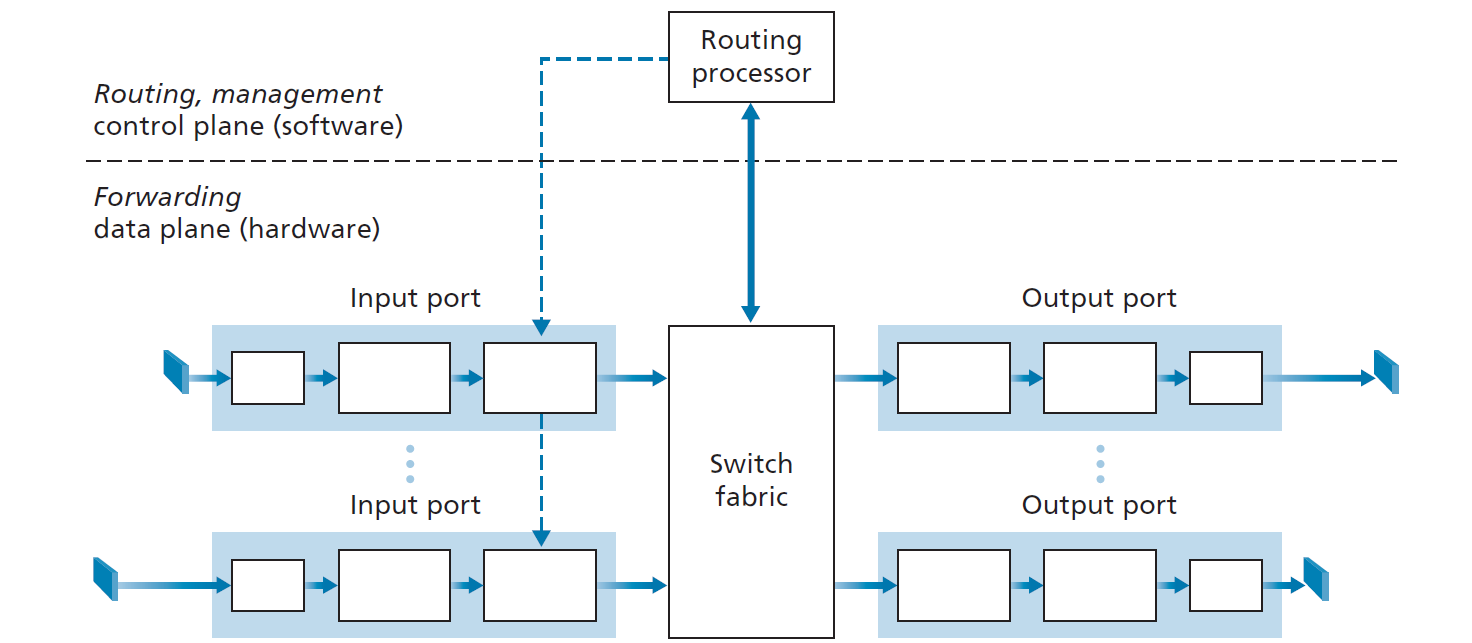
\includegraphics[keepaspectratio, width=14cm, height=11cm]{imagens/14/14 - Roteador.png}
\caption{Arquitetura de um roteador \\
Imagem retirada de: Computer Networking a top-down approach. 8th
ed.~Pearson, página 311. \\}
\label{Arquitetura de um roteador}
\end{figure}



\hypertarget{Descrição}{%
\section{Descrição}\label{Descrição}}

De forma mais descritiva, o roteador é composto por:

\begin{enumerate}
\def\labelenumi{\arabic{enumi}.}
\tightlist
\item
  \emph{input ports}: armazena os \emph{datagrams} recém chegados e
  performa funções da camada física e de enlace, como o \emph{lookup}, a
  determinação da porta de saída (para tal, é necessário consultar a
  \emph{fowarding table}).
\item
  \emph{Switching fabric}: conecta os \emph{input ports} com os
  \emph{Output ports}.
\item
  \emph{Output ports}: armazena os \emph{datagrams} recebidos pela
  \emph{Switching fabric} e transmite-os para fora do roteador
  (performando funções da camada física e de enlace essenciais).
\item
  \emph{Routing processor}: performa funções do \emph{control plane},
  como computar as rotas e manter a \emph{fowarding table} (em
  roteadores SDN, as operações mencionadas são feitas remotamente).
\end{enumerate}

É importante mencionar que os pontos 1, 2 e 3 são quase sempre
implementados em \emph{hardware}.

\hypertarget{tipos-de-forwarding}{%
\subsection{Tipos de forwarding}\label{tipos-de-forwarding}}

O \emph{output link} pode ser determinada de duas formas:

\begin{enumerate}
\def\labelenumi{\arabic{enumi}.}

\item
  \emph{Destination-based fowarding}: no qual a saída é baseada no
  destino.
\item
  \emph{Generalized forwarding}: em que o \emph{output link} é definido
  com base em N fatores, como a origem dos dados.
\end{enumerate}

Voltando para a analogia, o \emph{Destination-based fowarding} seria o
atendente do pedágio direcionar o carro a uma saída específica baseado
no destino que o motorista almeja. No caso do \emph{generalized
forwarding}, fatores como o tipo do veículo pode impactar na orientação
dada pelo atendente.

\hypertarget{questuxf5es-a-cerca-do-forwarding.}{%
\section{Questões a cerca do forwarding.}\label{questuxf5es-a-cerca-do-forwarding.}}

E se: 1. O atendente somente for capaz de atender 1 carro por minuto,
mas chegarem 2 carros por minuto ? 2. Todos os carros que entrarem forem
orientados para a mesma saída ? 3. Tiver mais carro entrando do que
saindo ? 4. For necessário tornar prioritário alguns veículos (como
ônibus) e bloquear a entrada de outros (como caminhões acima de um certo
peso) ?

Para as perguntas 1, 2 e 3, fica claro que gerará tráfego na entrada, na
saída e na via, respectivamente. Por fim, a resposta da pergunta 4 passa
pela criação de regras prévias a partir da definição das políticas de
filtro.

O mesmo pode ocorrer em um roteador, com a chegada de múltiplos
\emph{datagrams} em uma mesma \emph{input port} sendo maior que sua
capacidade de processá-los podendo gerar filas, atrasos e perda de dados
(com o mesmo ocorrendo na saída). A quantidade limitada de
\emph{datagrams} suportada pelo \emph{switch fabric} pode não suportar a
alta demanda de fluxo de dados, causando o bloqueio de novos entrantes
e, consequentemente, filas e atrasos.

Essas questões serão debatidas posteriormente em mais detalhes.

\hypertarget{input-port}{%
\section{Input Port}\label{input-port}}

A Figura \ref{Execuções na Input Port} mostra as execuções ocorridas na \emph{input port}.
Inicia-se com a ação de funções relativas a \emph{physical layer} (em
\emph{Line Termination}), seguida de funções da \emph{link layer} (em
\emph{Data link processing}), por fim o \emph{lookup, fowarding} e
\emph{queuing} (em \emph{lookup, fowarding, queuing}).





\begin{figure}[h!]
\centering
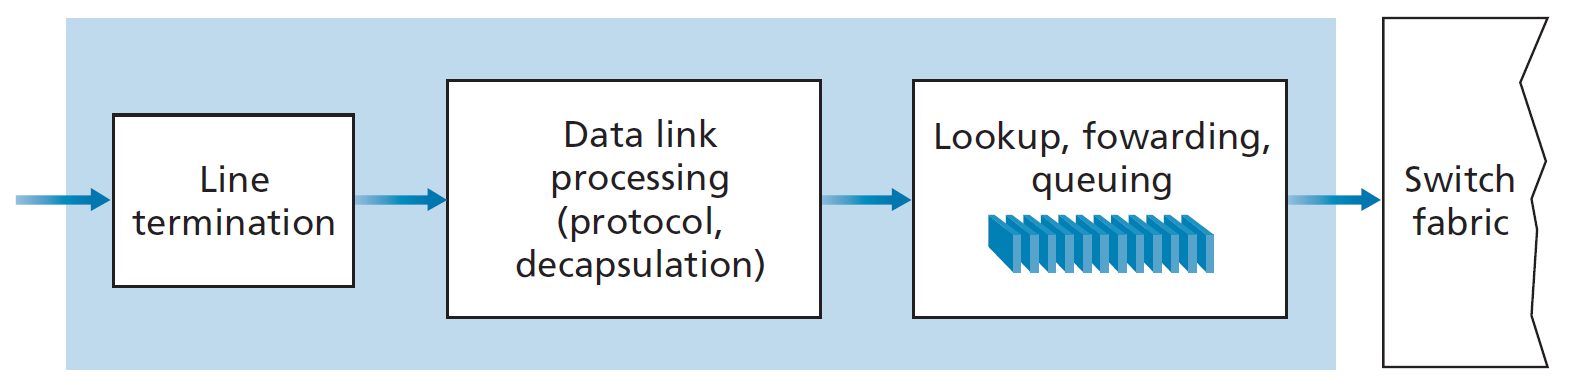
\includegraphics[keepaspectratio, width=12cm, height=9cm]{imagens/14/14 - input port.png}
\caption{Execuções na Input Port \\
Imagem retirada de: Computer Networking a top-down approach. 8th
ed.~Pearson, página 314. \\}
\label{Execuções na Input Port}
\end{figure}




A função central da porta de entrada é o \emph{lookup}, no qual o
roteador procura (\emph{look up}) na \emph{forwarding table} qual porta
o \emph{datagram} recém chegado deve ser direcionado. Apesar da
proeminente importância do \emph{lookup}, outras ações também devem ser
tomadas, como a checagem do \emph{version number}, \emph{checksum} e
\emph{Time to Live}

Como pode-se supor, em uma arquitetura de banco de dados centralizado,
os registros da \emph{forwarding table} estariam disponíveis em um único
local do roteador, com a operação de \emph{look up} devendo fazer uma
requisição de registro à esse banco de dados, algo que gera um possível
gargalo, afinal, caso o módulo do banco de dados não conseguir suprir a
demanda das requisições, deverão ocorrer filas e atrasos.

Para evitar esse gargalo, cada linha da tabela é copiada para cada um
dos \emph{input ports} presentes no roteador, de forma que o acesso à
tabela de transmissão (\emph{forwarding table}) seja feita localmente
(no \emph{input port}), sem a necessidade de requisições.

No \emph{look up}, o roteador identifica a saída (\emph{link interface})
utilizando a regra de maior correspondência (\emph{longest prefix
matching rule}) de prefixo do IP \emph{Address} de destino do
\emph{datagram}. Um exemplo dessas correspondências podem ser vistas na
Tabela 01. (O prefixo é formado por x primeiros dígitos do IP
\emph{Address} de destino referencia o endereço da sub-rede.)


\begin{table}[h!]
\centering
\begin{tabular}{||c c||} 
 \hline
    Prefix & Link Interface \\ [0.5ex] 
 \hline\hline
    11001000 00010111 00010 & 0 \\
 \hline
    11001000 00010111 00011000 & 1 \\
 \hline
    11001000 00010111 00011 & 2 \\
 \hline
    Prefix & Link Interface \\
 \hline

\end{tabular}
\caption{Exemplo de forwarding table \\}
\label{Exemplo de forwarding table}
\end{table}




Por exemplo, o endereço de IP:

\begin{verbatim}
11001000 00010111 00011000 10101010
\end{verbatim}

Tem o prefixo correspondendo ao \emph{link interface} 1 e 2, com o
\emph{link} 1 sendo a maior correspondência e, portanto, sendo os dados
direcionados ao mesmo.

\hypertarget{switching}{%
\section{Switching}\label{switching}}

O \emph{switching fabric} tem a função de conectar as \emph{input ports}
com as \emph{output ports}. Há diferentes formas de implementá-lo, mas
três delas, mostradas na Figura \ref{Tipos de Switching}, destacam-se:


\begin{figure}[h!]
\centering
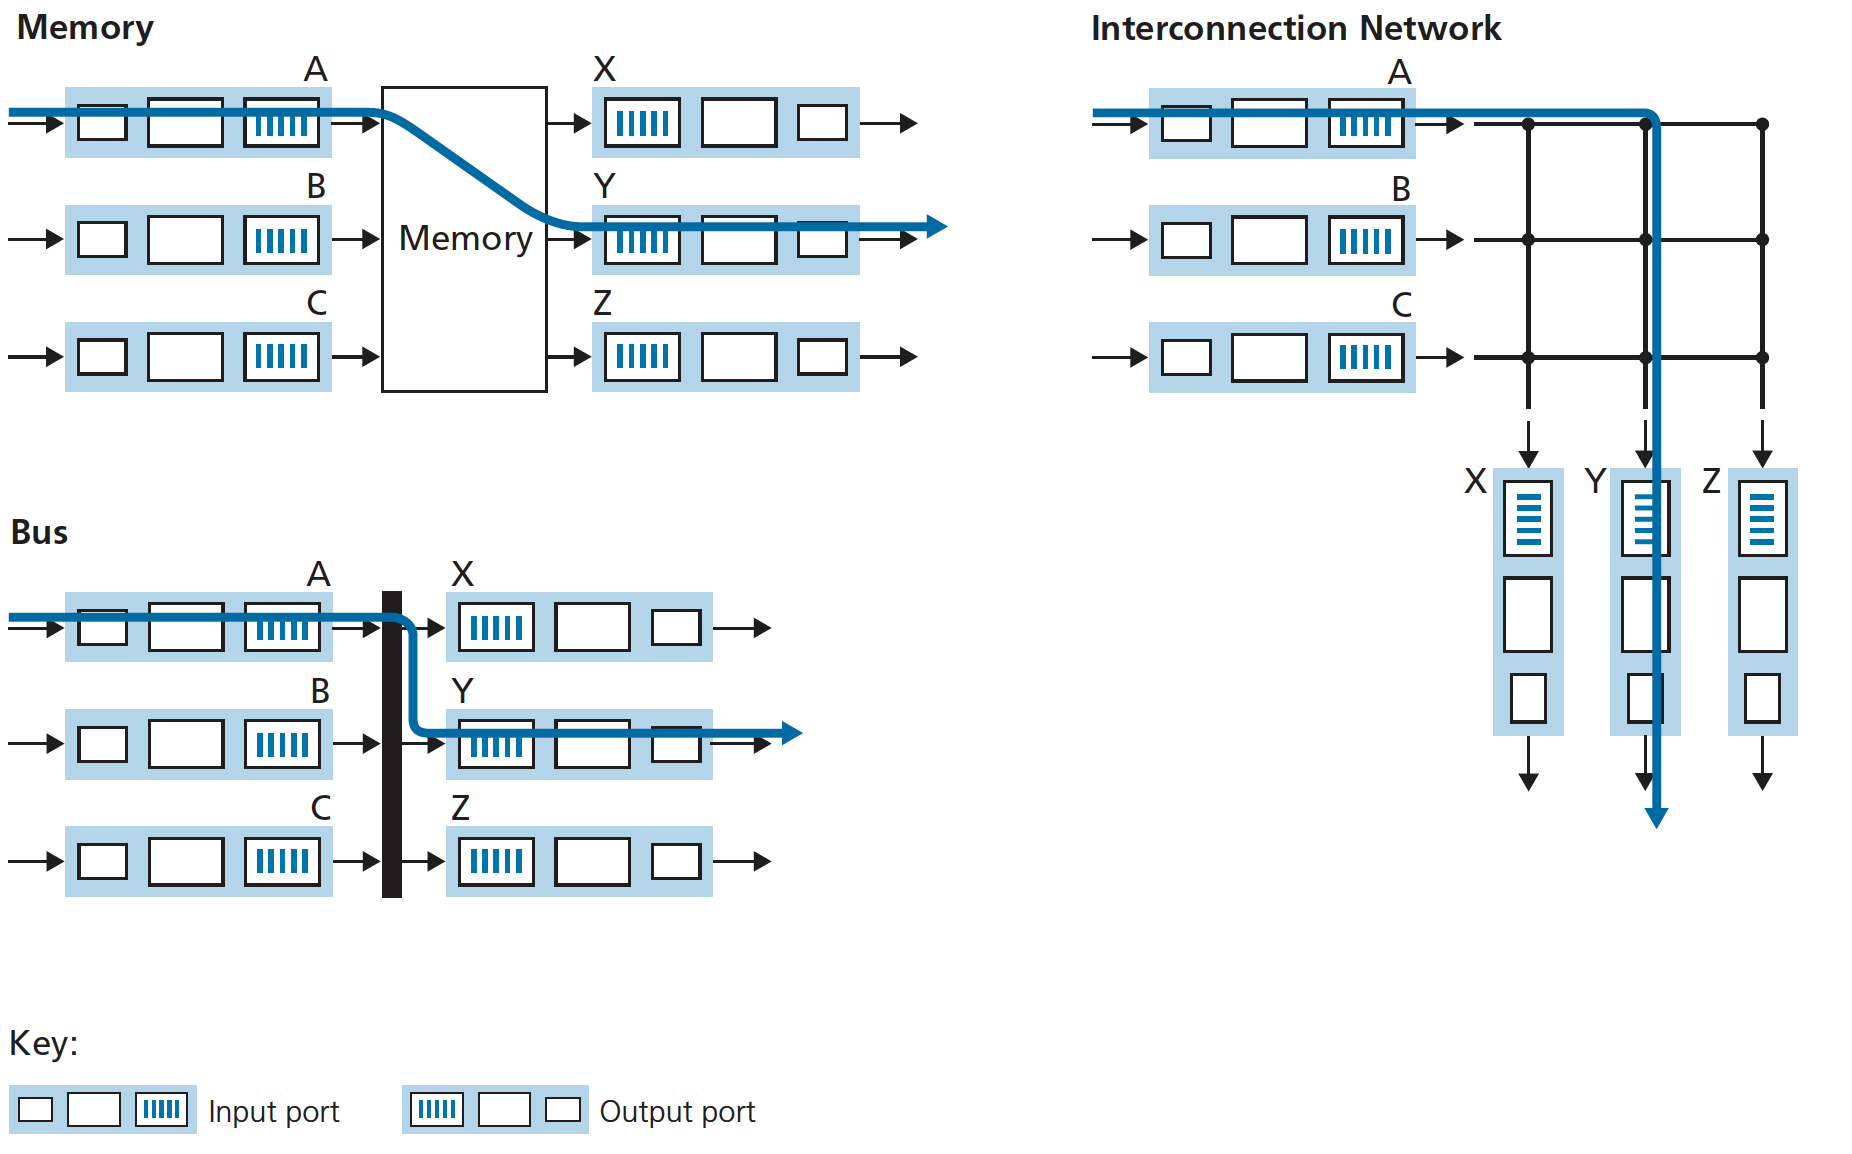
\includegraphics[keepaspectratio, width=16cm, height=13cm]{imagens/14/14 - switching.png}
\caption{Tipos de Switching \\
Imagem retirada de: Computer Networking a top-down approach. 8th
ed.~Pearson, página 317. \\}
\label{Tipos de Switching}
\end{figure}



\begin{enumerate}
\def\labelenumi{\arabic{enumi}.}

\item
  \emph{Switching via memory}: o \emph{input port} sinaliza, a partir de
  uma interrupção, para o processador do roteador a chegada de novos
  \emph{datagrams}. Após a interrupções, os dados recém chegados são
  copiados para a memória, processados (determinando-se a interface
  apropriada), e por fim copiados para o \emph{buffer} de saída. Isso é
  usualmente feito com processos com memória compartilhada.Como
  desvantagem pode-se citar, primeiro, a impossibilidade de transmissão
  de mais de um \emph{datagram} ao mesmo tempo, pois somente uma
  operação de leitura e escrita na memória pode ser feita por vez.
  Segundo, com a largura de banda sendo B \emph{datagrams} por segundo
  para memória (B \emph{datagrams} podem ser escritos ou lidos em 1
  segundo), significa dizer que a taxa de transferência está limitada em
  B/2 (pois será necessário fazer 1 operação de escrita e uma de
  leitura).
\item
  \emph{Switching via bus}: a \emph{input port} envia os
  \emph{datagrams} diretamente para a sua respectiva \emph{output port}
  através de um barramento compartilhado, sem a intervenção do
  processador do roteador. Isso é usualmente feito agregando-se um
  \emph{header} com um rótulo informando sua respectiva interface. Ao
  ser transmitido, todas as interfaces recebem esses dados, porém
  somente aquela indicada pelo rótulo irá manter o mesmo, retirando o
  seu rótulo, processando-o, e transmitindo-o para fora do roteador. O
  primeiro fato inconveniente dessa arquitetura é que somente 1 pacote de
  dados podem pecorrer o barramento. Isso significa que se chegarem
  múltiplos \emph{datagrams} em diferentes \emph{input ports}, todos
  menos 1 devem esperar o barramento tornar-se disponível. O segundo
  problema é que a velocidade do roteador estará limitada pela
  velocidade do barramento barramento. Esse tipo de arquitetura é
  indicado para LAN.
\item
  \emph{Switching via an interconnection network}: também chamado de
  cruzamento de barras, esse tipo de switch, como mostrado na Figura 02,
  pode alternar cada cruzamento de barra (ou nó) entre aberto e fechado
  de forma independente. Dessa maneira, multiplos \emph{datagrams} podem
  atravessar em paralelo o \emph{switch fabric} ao mesmo (ou seja,
  \emph{non-blocking} para uma \emph{output port} específica). Por
  exemplo, para emitir um dado do \emph{input} A para o \emph{output} Y,
  basta fechar o cruzamento dos mesmos. Esse fechamento não impedirá que
  os dados do \emph{input} B alcance a saída X, porém o \emph{output} Y
  estará somente disponível para o \emph{input} A (estando bloqueado
  para os outros \emph{inputs}).
\end{enumerate}

\hypertarget{output-port}{%
\section{Output port}\label{output-port}}

A Figura \ref{fig:Output Port} mostra as 3 principais execuções do \emph{output port}.
Inicia-se com o enfileiramento (\emph{Queuing}) dos \emph{datagrams}
recebidos. Em seguida, são performados ações necessárias relativas as
camadas físicas e enlace (\emph{Data link processing}). Por fim, os
dados são enviados para fora do roteador (\emph{Line termination}).


\begin{figure}[h!]
\centering
\includegraphics[keepaspectratio, width=12cm, height=9cm]{imagens/14/14 - output port.png}
\caption{Output Port \\
Imagem retirada de: Computer Networking a top-down approach. 8th
ed.~Pearson, página 319. \\}
\label{fig:Output Port}
\end{figure}


\hypertarget{filas}{%
\section{Filas}\label{filas}}

As filas podem se formar na entrada e na saída do roteador.

As filas na entrada podem ser formadas pela diferença de velocidade
entre o \emph{input} e o \emph{switching fabric} (como citado
anteriormente, de forma análoga, na questão 1 do ``E se'' no tópico''
Questões a a cerca do forwarding''). Se um \emph{input} for capaz de
lidar com uma taxa de \emph{datagrams} mais alta do que o
\emph{switching fabric}, os mesmos ficarão acumulados na entrada até
serem executados pelo \emph{switching fabric}.

Um outro evento que têm como consequência a geração de filas é o chamado
\emph{head-of-the-line blocking} (HOL \emph{blocking}). A Figura \ref{fig:Hol Blocking}
mostra um exemplo de como o HOL \emph{blocking} pode ocorrer. Os
\emph{datagrams} azuis-escuros estão destinados às saídas superiores,
enquanto que os azuis-claros estão destinados às saídas centrais. Assim,
um azul-escuro oriundo do \emph{input} superior pode bloquear a passagem
do \emph{datagram} azul-escuro oriundo do \emph{input} inferior,
travando a fila e impedindo que o \emph{datagram} azul-claro seja
processado paralelamente, apesar do caminho até sua saída estar livre.


\begin{figure}[h!]
\centering
\includegraphics[keepaspectratio, width=14cm, height=11cm]{imagens/14/14 - hol blocking.png}
\caption{Hol Blocking \\
Imagem retirada de: Computer Networking a top-down approach. 8th
ed.~Pearson, página 321. \\}
\label{fig:Hol Blocking}
\end{figure}


Na saída, as filas podem se formar quando múltiplos \emph{datagrams} dos
\emph{inputs} são direcionados para o mesmo \emph{output}, como mostrado
na Figura \ref{fig:Fila na saída}. Esse evento pode preencher o \emph{buffer} de saída,
ocasionando a ``derrubada'' de novos \emph{datagrams}, política chamada
de \emph{drop-tail}, ou a remoção de um já enfileirado, para assim criar
espaço para os dados recém chegados. Em alguns casos, pode ser vantajoso
remover um pacote de dados antes que fila fique cheia, de forma a enviar
um sinal de congestionamento para o emissor. Os algoritmos responsáveis
por isso são chamados de \emph{Active Queue Management} (AQM), ou
gerenciador de filas ativo, com o \emph{Random Early Detection} (RED)
sendo um algoritmo dessa classe amplamente implementado.


\begin{figure}[h!]
\centering
\includegraphics[keepaspectratio, width=12cm, height=9cm]{imagens/14/14 - output queue.png}
\caption{Fila na saída \\
Imagem retirada de: Computer Networking a top-down approach. 8th
ed.~Pearson, página 322. \\}
\label{fig:Fila na saída}
\end{figure}




O tamanho do espaço destinado para as filas sofrem de uma dicotomia.
Enquanto que \emph{buffers} pequenos podem não apresentar espaço
suficiente para lidar com picos de demanda, algo que aumenta o número de
dados perdidos, filas grandes podem representar um longo tempo de
espera, aumentando o atraso na entrega dos \emph{datagrams}.

Para equilibrar esses diferentes pontos, o tamanho do \emph{buffer}
(\texttt{B}) fora relacionado com o \emph{round-trip time} (RTT) médio
(período entre a emissão dos dados e a recepção do seu ACK) e a
capacidade do link (\texttt{C}).

\begin{verbatim}
B = RTT . C

B = 2.5G bits, para RTT = 250 ms, e C = 10 Gbps
\end{verbatim}

Atualmente, também relaciona-se o número de fluxos independentes de TCP
(\texttt{N}):

\begin{verbatim}
B = RTT . C / sqrt{N} 
\end{verbatim}

\hypertarget{prioridades-dos-dados}{%
\section{Prioridades dos dados}\label{prioridades-dos-dados}}

Na discussão dos \emph{buffers} fora deixado implícito a política
\emph{First-in-First-Out} (FIFO), ou primeiro a chegar, primeiro a sair
(modelo mostrado na Figura \ref{fig:Modelo FIFO}), mas outras regras também podem ser
utilizadas, como a classificação dos dados em diferentes filas a partir
de sua prioridade (modelo mostrado na Figura \ref{fig:Modelo classificação e priorização}).


\begin{figure}[h!]
\centering
\includegraphics[keepaspectratio, width=12cm, height=9cm]{imagens/14/14 - FIFO.png}
\caption{Modelo FIFO \\
Imagem retirada de: Computer Networking a top-down approach. 8th
ed.~Pearson, página 325. \\}
\label{fig:Modelo FIFO}
\end{figure}




\begin{figure}[h!]
\centering
\includegraphics[keepaspectratio, width=12cm, height=9cm]{imagens/14/14 - priority queue.png}
\caption{Modelo classificação e priorização \\
Imagem retirada de: Computer Networking a top-down approach. 8th
ed.~Pearson, página 326. \\}
\label{fig:Modelo classificação e priorização}
\end{figure}

Uma forma generalizada de classificação e priorização dos dados que tem
sido bastante implementada é o chamada de \emph{Weighted Fair Queuing}
(WFQ), na qual as filas de maior peso são tratadas primeiro, seguindo
para as de menor peso, até reiniciar o ciclo, como mostrado na Figura
\ref{fig:Weighted Fair Queuing}.


\begin{figure}[h!]
\centering
\includegraphics[keepaspectratio, width=12cm, height=9cm]{imagens/14/14 - WFQ.png}
\caption{Weighted Fair Queuing \\
Imagem retirada de: Computer Networking a top-down approach. 8th
ed.~Pearson, página 326. \\}
\label{fig:Weighted Fair Queuing}
\end{figure}



\hypertarget{neutralidade-das-redes}{%
\subsection{Neutralidade das redes}\label{neutralidade-das-redes}}

Como qualquer regra pode ser imposta para a classificação dos dados, os
ISP's podem não ser neutros no oferecimento de seus serviços, algo que
vem resultando leis que regulamentam o que os ISP's podem ou não fazer.

Em geral, a defesa da neutralidade das redes pode ser resumido em 3
pontos:

\begin{enumerate}
\def\labelenumi{\arabic{enumi}.}
\tightlist
\item
  Conteúdos não devem ser bloqueados (\emph{No Blocking}).
\item
  Tráfico de Internet não deve ser penalizado (\emph{No Throttling}).
\item
  Não deve haver priorização paga (\emph{Paid Prioritization}).
\end{enumerate}

\hypertarget{generalized-forwarding}{%
\chapter{Generalized Forwarding}\label{generalized-forwarding}}

O \emph{Generalized Forwarding} é a forma genérica do paradigma
\emph{match plus action}, no qual utiliza os \emph{headers} associados
aos protocolos de diferentes camadas para determinar o que deve ser
feito com os dados recebidos. Para a sua implementação, é utilizado o
padrão OpenFlow, o qual baseia-se no SDN (\emph{Software Defined
Network}), que aplica um controlador remoto para o cálculo das regras da
rede.

A base do \emph{Generalized Forwarding} está na \emph{Flow Table},
tabela no qual está contido as regras do \emph{match plus action}. Cada
regra têm:

\begin{enumerate}
\def\labelenumi{\arabic{enumi}.}
\tightlist
\item
  Um conjunto de \emph{headers} à serem verificados.
\item
  Um conjunto de contadores.
\item
  Um conjunto de ações à serem tomadas.
\end{enumerate}

Perceba que essa tabela é uma forma limitada de programação. Atualmente,
vem ganhando força uma alternativa mais rica de possibilidades de
implementação (com variáveis e funções), a linguagem \emph{Programming
Protocol-independent Packet Processors} (P4).

Dentro do padrão OpenFlow, os \emph{headers} podem ser oriundos das
camadas de enlace, rede e transporte, como mostrado na Figura \ref{fig:OpenFlow Headers}. É
importante perceber que nem todos os \emph{headers} podem ser escolhidos
para a ação de correspondência (\emph{match}) (assim fora implementado
como uma forma de equilibrar a funcionalidade e complexidade. É melhor
fazer algo simples e bem, do que muita coisa e ruim).


\begin{figure}[h!]
\centering
\includegraphics[keepaspectratio, width=12cm, height=9cm]{imagens/14/14 - Open Flow headers.png}
\caption{OpenFlow Headers \\
Imagem retirada de: Computer Networking a top-down approach. 8th
ed.~Pearson, página 356. \\}
\label{fig:OpenFlow Headers}
\end{figure}



As ações a serem tomadas são:

\begin{enumerate}
\def\labelenumi{\arabic{enumi}.}
\tightlist
\item
  \emph{Forwarding}: a transmissão dos dados.
\item
  \emph{Dropping}: o ``deixar de lado''.
\item
  \emph{Modify-field}: a modificação de algum \emph{header}.
\end{enumerate}

\hypertarget{camada-de-rede-control-plane}{%
\section{Camada de rede: Control Plane}\label{camada-de-rede-control-plane}}

Na aula anterior, foi debatido a importância da \emph{Fowarding Table}
para o \emph{Data Plane}. Os dados registrados nessa tabela são
computados pela \emph{Control Plane}, a qual tem como objetivo controlar
a rota global que os \emph{datagrams} precisarão percorrer para sair de
uma ponta à outra da rede (end-to-end). A \emph{Control Plane} também
configura e gerencia os componentes e serviços fornecidos pela camada de
rede.

Uma rede pode ser vista como um grafo, no qual os vértices (ou nós) são
os roteadores e as arestas são a conexão entre dois vértices, como pode
ser visto na Figura \ref{fig:Grafo com pesos}. Dessa forma, os algoritmos de roteamento
determinam o melhor caminho que um dado pode percorrer para sair de um
vértice da rede até outro vértice.

\begin{figure}[H]
\centering
\includegraphics[keepaspectratio, width=12cm, height=9cm]{imagens/14/14 - grafo.png}
\caption{Grafo com pesos \\
Imagem retirada de: Computer Networking a top-down approach. 8th
ed.~Pearson, página 381. \\}
\label{fig:Grafo com pesos}
\end{figure}

As características de cada conexão (velocidade, tarifas financeiras,
etc.) são contabilizadas (a partir de métricas estabelecidas pela
instituição dona da rede), resultando no custo (ou peso) agregado à
conexão. Como cada aresta apresenta características diferentes, serão
agregados pesos diferentes ao uso de cada uma. Assim, os algoritmos de
roteamento, como o OSPF e o BGP (conhecido como a ``cola'' da Internet),
tem o objetivo de encontrar um caminho entre dois nós que apresente o
menor custo de ser percorrido (custo total do caminho).




É importante perceber que o caminho de menor custo (\emph{least-cost
path}) é diferente do caminho mais curto (\emph{shortest path}), pois o
primeiro é caracterizado por aquele que apresenta o menor somatório dos
pesos das conexões inseridas no mesmo, enquanto que o segundo é
determinado pela menor quantidade de nós que deve ser percorrido.

Ambos os algoritmos citados (OSPF e BGP) utilizam a abordagem
\emph{per-router control} (mostrado na Figura \ref{fig:Per Router Control}), em que o algoritmo de
roteamento é processado dentro de cada roteador, sendo necessário
interações entre \emph{routers} para a determinação das rotas. Outra
possível abordagem é a \emph{Logically centralized control} (mostrado na
Figura \ref{fig:Logically Centralized Controller}), em que há uma centralização computação em um servidor e
distribuição dos parâmetros determinados para os nós da rede, como
adotado pelo SDN (\emph{Software Defined Network}).


\begin{figure}[h!]
\centering
\includegraphics[keepaspectratio, width=12cm, height=9cm]{imagens/14/14 - per router control.png}
\caption{Per Router Control \\
Imagem retirada de: Computer Networking a top-down approach. 8th
ed.~Pearson, página 378. \\}
\label{fig:Per Router Control}
\end{figure}



\begin{figure}[h!]
\centering
\includegraphics[keepaspectratio, width=12cm, height=9cm]{imagens/14/14 - Logically centralized controller.png}
\caption{Logically Centralized Controller \\
Imagem retirada de: Computer Networking a top-down approach. 8th
ed.~Pearson, página 379. \\}
\label{fig:Logically Centralized Controller}
\end{figure}




\hypertarget{Classificação dos algoritmos}{%
\section{Classificação dos algoritmos}\label{Classificação dos algoritmos}}

De forma abrangente, podemos classificar os algoritmos de roteamento em:

\begin{enumerate}
\def\labelenumi{\arabic{enumi}.}
\item
  \emph{Centralized routing algorithm}: os algoritmos dessa categoria,
  comumente referidos como \emph{link-state} (LS) \emph{algorithms},
  computam o caminho a partir de um conhecimento completo a cerca da
  conectividade e custos de cada conexão da rede (tendo um conhecimento
  global da rede). Um exemplo é o algoritmo de Dijkstra.
\item
  \emph{Decentralized routing algorithm}: a determinação do caminho de
  menor custo é feita de forma iterativa e distribuída em cada roteador.
  Como, inicialmente, cada roteador só têm conhecimento dos custos de
  seus próprios \emph{links}, o cálculo do menor caminho necessitará da
  troca de informações entre os outros roteadores da rede. Isso ocorre
  de forma iterativa e gradual. Um exemplo é o \emph{Distance-Vector
  Routing Algorithm} (DV), um algoritmo iterativo, assíncrono e
  distribuído, com cada nó mantendo um vetor de estimativas de custos de
  todos os outros nós da rede (com a atualização ocorrendo conforme
  mudanças na rede acontecem). Podemos citar alguns protocolos que
  utilizam o DV: Internet's RIP, BGP, ISO IDRP, Novel IPX e o original
  ARPAnet.
\end{enumerate}

Uma segunda forma de classificação é:

\begin{enumerate}
\def\labelenumi{\arabic{enumi}.}
\tightlist
\item
  \emph{Static Routing Algorithms}: os roteadores mudam muito pouco no
  decorrer do tempo (frequentemente como resultado de uma intervenção
  humana).
\item
  \emph{Dynamic routing algorithms}: as rotas mudam conforme a ocorre
  mudança na topologia da rede ou carga de tráfego (apesar dessa
  categoria apresentar maior responsividade em mudanças na rede, também
  estão mais suscetíveis a problemas como \emph{loops} e oscilações).
\end{enumerate}

Uma terceira forma:

\emph{Load-Sensitive algorithm}: os custos dos \emph{links} variam
dinamicamente conforme o nível de congestionamento.
\emph{Load-Insensitive algotihm}: os custos dos \emph{links} não
refletem explicitamente o nível de congestionamento.

\hypertarget{ls-vs-dv}{%
\section{LS vs DV}\label{ls-vs-dv}}

Alguns pontos são importantes para a comparação entre os
\emph{link-state algorithms} e o \emph{Distance-Vector Routing
Algorithm}:

\begin{enumerate}
\def\labelenumi{\arabic{enumi}.}
\item
  \emph{Message complexity}: o LS requer que cada nó saiba os custos de
  cada conexão da rede, com uma mudança em um custo devendo ser enviada
  para todos os nós. Já no DV, o envio do novo custo somente ocorre
  quando o mesmo impacta no caminho de menor custo dos nós anexados ao
  \emph{link} relativo à alteração (DV melhor que LS).
\item
  \emph{Speed of convergence}: LS converge mais rápido do que o DV (LS
  melhor que DV).
\item
  \emph{Robustness}: no DV, um caminho de menor custo calculado
  incorretamente por um nó será publicado para todos os nós da rede,
  diferentemente do LS, no qual os caminhos são calculados em cada nó,
  provendo assim um certo nível de robustez (LS melhor que DV).
\end{enumerate}

\hypertarget{intra-autonomous-sistems-routing-ospf}{%
\section{Intra-Autonomous Sistems Routing: OSPF}\label{intra-autonomous-sistems-routing-ospf}}

Um sistema autônomo (Autonomous Sistems, AS) consiste de um conjunto de
roteadores que estão sob um mesmo controle administrativo. Isso torna
possível a escalabilidade e a autonomia administrativa do sistema. Os
algoritmos de roteamento que rodam em um AS são chamados de
\emph{intra-autonomous system routing protocol}. Um exemplo de algoritmo
é o \emph{Open Shortest Path First}, um protocolo LS no qual as
especificações do protocolo de roteamento está disponível publicamente
(a parte \emph{Open} do nome). No OSPF, cada roteador monta um mapa
topológico completo de todo o AS, e então executa o algoritmo de
Dijkstra para a determinação da árvore de caminhos de menor custo para
todas as sub-redes, com os custos das conexões sendo configurados pelo
administrador da rede.

Observe que is roteadores que conectam-se com outros de diferentes ASs
são chamados de \emph{gateway routers} (eles estão nos limites da AS).
Já aqueles que estão no interior da AS, são chamados de \emph{internal
routers}.

Alguns pontos importantes de mencionar:

\begin{enumerate}
\def\labelenumi{\arabic{enumi}.}
\item
  \emph{Security}: as trocas de informações entre os roteadores OSPF
  podem ser autenticadas por meio da geração de um \emph{hash} MD5
  (utilizando-se uma chave secreta, que está contida no roteador e não é
  compartilhada) por ambos (emissor e receptor da mensagem). Em seguida
  o \emph{hash} do emissor é comparado com o do receptor. O emissor pode
  ser considerado autêntico caso os \emph{hashs} gerados sejam iguais.
  Caso contrário, a mensagem dese ser ignorada.
\item
  \emph{Multiple same-cost path}: O tráfego de dados poderá ser
  distribuído em todas as rotas que contenham o custo mínimo.
\item
  \emph{Support for hierarchy within a single AS}: o sistema pode ser
  configurado hierarquicamente em áreas.
\end{enumerate}

\hypertarget{inter-autonomous-sistems-routing-bgp}{%
\section{Inter-Autonomous Sistems Routing: BGP}\label{inter-autonomous-sistems-routing-bgp}}

Por necessitar a coordenação de múltiplos ASs, a comunicação entre ASs
deve ocorrer utilizando-se o mesmo protocolo. O protocolo usado é o
\emph{Border Gateway Protocol} (BGP), e é conhecido também por ser a
``cola'' da Internet (por unir os diferentes ASs).

O roteamento pelo BGP ocorre entre sub-redes e não para um endereço
específico da rede. Dessa forma, a \emph{forwarding table} do roteador
toma a forma de \texttt{(x,\ I)}, onde \texttt{x} é o prefixo e o
\texttt{I} é a interface do roteador.

O BGP provê para os roteadores meios para:

\begin{enumerate}
\def\labelenumi{\arabic{enumi}.}
\tightlist
\item
  Obter o prefixo de AS vizinhos: com a publicação da existência de cada
  rede para o resto da Internet.
\item
  Determinar a melhor rota para cada prefixo: no qual a melhor rota é
  baseada nas políticas determinadas pelo administrador da rede e na
  acessibilidade da informação.
\end{enumerate}

As conexões BGP entram em duas categorias (graficamente representado na
Figura \ref{fig:eBGP e iBGP}):

\begin{enumerate}
\def\labelenumi{\arabic{enumi}.}
\tightlist
\item
  iBGP (\emph{internal} BGP): conexão BGP internas aos ASs
\item
  eBGP (\emph{external} BGP): conexão externa aos ASs (entre ASs)
\end{enumerate}


\begin{figure}[h!]
\centering
\includegraphics[keepaspectratio, width=12cm, height=9cm]{imagens/14/14 - eBGP e iBGP.png}
\caption{eBGP e iBGP \\
Imagem retirada de: Computer Networking a top-down approach. 8th
ed.~Pearson, página 402. \\}
\label{fig:eBGP e iBGP}
\end{figure}



A publicação no BGP ocorre de forma bem direta. A Figura \ref{fig:ASs com adição de x} mostra a
adição de uma sub-rede (\texttt{x}) em uma rede com 3 ASs. Primeiro o AS3
envia uma BGP \emph{message} (\texttt{AS3\ x}) para o AS2 dizendo que a
sub-rede \texttt{x} existe e é acessível através dele. Em seguida, o AS2
avisa para o AS1 a existência de \texttt{x} e que o mesmo é acessível
através do caminho AS2-AS3 (\texttt{AS2\ AS3\ x}).


\begin{figure}[h!]
\centering
\includegraphics[keepaspectratio, width=12cm, height=9cm]{imagens/14/14 - SAs com a adicao de x.png}
\caption{ASs com adição de x \\
Imagem retirada de: Computer Networking a top-down approach. 8th
ed.~Pearson, página 401. \\}
\label{fig:ASs com adição de x}
\end{figure}



O BGP \emph{message} é composto pelo prefixo e outros múltiplos
atributos, como o \emph{AS-PATH}, que explicita a lista de ASs na qual a
mensagem publicação de existência da nova rede precorreu (como mostrado
no exemplo anterior), e \emph{NEXT-HOP}, que é o endereço da interface
do roteador que inicia a o \emph{AS-PATH}.

\hypertarget{hot-potato}{%
\section{Hot Potato}\label{hot-potato}}

Os ASs operam com a bordagem \emph{Hot Potato}, o qual os roteadores
objetivam transmitir os dados para fora do AS o mais rápido possível.
Para tal, o roteador com os dados disparará para o endereço do
\emph{NEXT-HOP} que tiver o menor custo de conexão, sem se preocupar com
o resto do trajeto desses dados. Assim, apesar de localmente eficiente,
a rota global escolhida pode não ser a mais rápida. A Figura \ref{fig:Duas possibilidades de NEXT-HOP} mostra
duas possibilidades de \emph{NEXT-HOP}. A rota escolhida será aquela que
apresentar o menor custo de conexão relacionado ao \emph{NEXT-HOP}. A
Figura \ref{fig:Passos para a adição de um destino externo na forwarding
table} mostra os passos para a adição de um destino externo ao AS na
\emph{forwarding table}

\begin{figure}[h!]
\centering
\includegraphics[keepaspectratio, width=12cm, height=9cm]{imagens/14/14 - rota com menor next-hop.png}
\caption{Duas possibilidades de NEXT-HOP \\
Imagem retirada de: Computer Networking a top-down approach. 8th
ed.~Pearson, página 403. \\}
\label{fig:Duas possibilidades de NEXT-HOP}
\end{figure}

\begin{figure}[h!]
\centering
\includegraphics[keepaspectratio, width=12cm, height=9cm]{imagens/14/14 - adicao destino.png}
\caption{Passos para a adição de um destino externo na forwarding
table \\
Imagem retirada de: Computer Networking a top-down approach. 8th
ed.~Pearson, página 404. \\}
\label{fig:Passos para a adição de um destino externo na forwarding
table}
\end{figure}


\hypertarget{Seleção da rota.}{%
\section{Seleção da rota.}\label{Seleção da rota.}}

Na prática, a rota selecionada utiliza outros parâmetros além do
\emph{Hot Potato}:

\begin{enumerate}
\def\labelenumi{\arabic{enumi}.}
\tightlist
\item
  Política de decisão da preferência local de transmissão: essa política
  é escolhida pelo administrador da rede
\item
  Para os restantes, será escolhido o que tiver o menor \emph{AS-PATH}.
\item
  Para os restantes, o \emph{Hot Potato} entra em ação, escolhendo a
  rota com o menor custo de transmissão para o \emph{NEXT-HOP}.
\item
  Para os restantes, é utilizado os identificadores BGP para a seleção
  da rota.
\end{enumerate}

\hypertarget{poluxedtica-de-preferuxeancia-local-e-protocolos-intra-vs-inter}{%
\section{Política de preferência local e Protocolos Intra vs Inter}\label{poluxedtica-de-preferuxeancia-local-e-protocolos-intra-vs-inter}}

O AS é dito como sistema autônomo pois o mesmo apresenta uma
independência administrativa. Isso é algo que pode gerar alguns
problemas de confiança, com decisões como não permitir que dados
originário de um AS passe através de outro AS específico. E, de forma
similar, um AS pode ter interesse em querer controlar o tráfego de dados
entre outros ASs. Um reflexo no cenário atual é a desconfiança dos
americanos sob empresas chinesas, que, comumentemente, recebe
interferência do governo chinês, um inimigo declarado dos EUA (assim,
deve-se ser evitado que dados críticos do governo americanos sejam
transmitidos através de empresas chinesas).

Outra questão gira em torno do problema de uma sub-rede de um cliente
fazer parte da rota dos dados de outros clientes. Um cliente deve ser
origem ou destino das mensagens e não um meio.

A política é uma questão tão forte na comunicação inter-ASs, que ela é
um dos maiores motivos para que os protocolos inter-ASs sejam diferentes
dos intra-ASs, tanto que até a qualidade das rotas (externas) utilizadas
é uma preocupação secundária. Por fim, a questão da escala não é tão
forte no intra-ASs quanto é em inter-ASs. Assim, os 3 motivos para que
os protocolos sejam diferentes são:

\begin{enumerate}
\def\labelenumi{\arabic{enumi}.}
\tightlist
\item
  Política: intra-ASs é secundário, inter-ASs é primário.
\item
  Escala: intra-ASs é secundário, inter-ASs é primário.
\item
  Performance: intra-ASs é primário, inter-ASs é secundário (impactado
  pelas políticas).
\end{enumerate}

\end{document}